\documentclass[a4paper]{article}

\usepackage[utf8]{inputenc}
\usepackage[T1]{fontenc}
\usepackage{textcomp}
\usepackage[italian]{babel}
\usepackage{amsmath, amssymb}
\usepackage{amsfonts}
\usepackage{mdframed}
\usepackage{float}
\usepackage{xcolor}
\usepackage{listings}
\usepackage{graphicx}
\usepackage{tikz}
\usetikzlibrary{shapes, arrows, automata, petri, positioning, calc}
\usepackage{circuitikz}
\usepackage[label=corner]{karnaugh-map}
\graphicspath{{./figures/}}

\usepackage{ntheorem}
\newtheorem{theorem}{Teorema}

\usepackage{import}
\usepackage{pdfpages}
\usepackage{transparent}
\usepackage{xcolor}

% Code blocks
\definecolor{codegreen}{rgb}{0,0.6,0}
\definecolor{codegray}{rgb}{0.5,0.5,0.5}
\definecolor{codepurple}{rgb}{0.58,0,0.82}
\definecolor{backcolour}{rgb}{0.95,0.95,0.95}

\lstdefinestyle{mystyle}{
	backgroundcolor=\color{backcolour},
	commentstyle=\color{codegreen},
	keywordstyle=\color{magenta},
	numberstyle=\tiny\color{codegray},
	stringstyle=\color{codepurple},
	basicstyle=\ttfamily\footnotesize,
	breakatwhitespace=false,
	breaklines=true,
	captionpos=b,
	keepspaces=true,
	numbers=left,
	numbersep=5pt,
	showspaces=false,
	showstringspaces=false,
	showtabs=false,
	tabsize=2
}

\lstset{style=mystyle}

\usepackage{color}

\definecolor{dkgreen}{rgb}{0,0.6,0}
\definecolor{gray}{rgb}{0.5,0.5,0.5}
\definecolor{mauve}{rgb}{0.58,0,0.82}

\lstset{frame=tb,
	aboveskip=3mm,
	belowskip=3mm,
	showstringspaces=false,
	columns=flexible,
	basicstyle={\small\ttfamily},
	numbers=none,
	numberstyle=\tiny\color{gray},
	keywordstyle=\color{blue},
	commentstyle=\color{dkgreen},
	stringstyle=\color{mauve},
	breaklines=true,
	breakatwhitespace=true,
	tabsize=3
}

\usepackage{import}
\usepackage{pdfpages}
\usepackage{transparent}
\usepackage{xcolor}



% Useful definitions frame
\theoremstyle{break}
\theoremheaderfont{\bfseries}
\newmdtheoremenv[%
	linecolor=gray,leftmargin=0,%
	rightmargin=0,
	innertopmargin=8pt,%
	innerbottommargin=8pt,
	ntheorem]{define}{Definizioni utili}[section]

% Example frame
\theoremstyle{break}
\theoremheaderfont{\bfseries}
\newmdtheoremenv[%
	linecolor=gray,leftmargin=0,%
	rightmargin=0,
	innertopmargin=8pt,%
	innerbottommargin=8pt,
	ntheorem]{example}{Esempio}[section]

% Important definition frame
\theoremstyle{break}
\theoremheaderfont{\bfseries}
\newmdtheoremenv[%
	linecolor=gray,leftmargin=0,%
	rightmargin=0,
	backgroundcolor=gray!40,%
	innertopmargin=8pt,%
	innerbottommargin=8pt,
	ntheorem]{definition}{Definizione}[section]

% Exercise frame
\theoremstyle{break}
\theoremheaderfont{\bfseries}
\newmdtheoremenv[%
	linecolor=gray,leftmargin=0,%
	rightmargin=0,
	innertopmargin=8pt,%
	innerbottommargin=8pt,
	ntheorem]{exercise}{Esercizio}[section]

% figure support
\usepackage{import}
\usepackage{xifthen}
\pdfminorversion=7
\usepackage{pdfpages}
\usepackage{transparent}
\newcommand{\incfig}[1]{%
	\def\svgwidth{\columnwidth}
	\import{./figures/}{#1.pdf_tex}
}

% FSM tikz
\tikzset{
    place/.style={
        circle,
        thick,
        draw=black,
        minimum size=6mm,
    },
        state/.style={
        circle,
        thick,
        draw=blue!75,
        fill=blue!20,
        minimum size=6mm,
    },
}

\pdfsuppresswarningpagegroup=1

\begin{document}

% Custom circuitikz components

% 2 bit adder
\tikzset{component adder/.style={flipflop,
 flipflop def={t1=B, t3=A, t5=S,
 td=cout, tu=cin},
 }}
\newcommand{\fulladder}[2] % #1 = name from to[generic,n=#1], #2 = rotation angle
{\draw[rotate=#2] (#1) 
  (0,0) node[component adder, rotate=-90+#2] {+}
;}

% Latch regisry
\tikzset{component registry/.style={flipflop,
 flipflop def={t2=I, t5=O,
 td=CK},
 }}
\newcommand{\registry}[2] % #1 = name from to[generic,n=#1], #2 = rotation angle
{\draw[rotate=#2] (#1) 
  (0,0) node[component registry, rotate=-90+#2] {\rotatebox{90}{REG}}
;}


% ------------------------------

\begin{titlepage}
	\begin{center}
		\vspace*{1cm}

		\Huge
		\textbf{Probabilità e Statistica\\Esercizi}

		\vspace{0.5cm}
		\LARGE
		UniVR - Dipartimento di Informatica

		\vspace{1.5cm}

		\textbf{Fabio Irimie}

		\vfill


		\vspace{0.8cm}


		2° Semestre 2023/2024

	\end{center}
\end{titlepage}


\tableofcontents
\pagebreak
\section{Introduzione}
L'informatica è nata per la risoluzione di problemi di calcolo, in particolare
quelli di calcolo numerico. Per questo motivo i primi computer erano macchine
che eseguivano operazioni aritmetiche. Per risolvere questi problemi si usano
degli algoritmi che sono una sequenza di istruzioni semplici che portano poi
a risolvere problemi di complessità variabile. Anche gli algoritmi hanno una
complessità che deve essere adeguata alla risoluzione del problema.

\subsection{Hardware}
Un algoritmo deve essere trasformato in un processo di calcolo automatico,
quindi deve essere implementato tramite hardware. Ci sono due tipi di hardware:
\begin{itemize}
	\item \textbf{Embedded} che è un hardware dedicato ad un singolo compito.
	      Ad esempio il microonde.
	\item \textbf{General purpose} non si sa l'utilizzo finale, quindi ha
	      funzionalità generali ampliate dal software installato. L'hardware
	      general purpose è programmabile attraverso il software. Un esempio
	      è il PC.
\end{itemize}

In base al tipo di hardware l'algoritmo viene implementato in diversi modi:
\begin{itemize}
	\item \textbf{Algoritmo} \( \to  \) \textbf{Software}: Tramite un linguaggio di programmazione
	\item \textbf{Algoritmo} \( \to  \)  \textbf{Hardware embedded}: Tramite linguaggi di basso livello
	      come C, Assembly o il sistema operativo.
	\item \textbf{Algoritmo} \( \to  \)  \textbf{Hardware}: Tramite sintesi logica
\end{itemize}

\subsection{Campionamento dei dati}
Ogni cosa nel mondo è rappresentabile da funzioni continue nel tempo \( f(t) \),
ma con risorse finite è impossibile rappresentare infiniti dati, bisogna quindi
campionarli.

\begin{figure}[h]
	\centering
	\begin{tikzpicture}[scale=0.6, domain=0:10]
		\coordinate (A) at (0,4);
		\coordinate (B) at (1,4);
		\coordinate (C) at (2,2);
		\coordinate (D) at (3,4);
		\coordinate (E) at (4,1);
		\coordinate (F) at (5,3);
		\coordinate (G) at (6,2);
		\coordinate (H) at (7,4);
		\coordinate (I) at (8,3);
		\coordinate (J) at (9,2);
		\coordinate (K) at (10,5);

		\draw [->] (0,0) -- (10,0) node[right] {$t$};
		\draw [->] (0,0) -- (0,5) node[above] {$f(t)$};

		\draw [gray!50, ultra thin] (0,0) grid (10,5);
		\draw [blue, ultra thick] plot [smooth, tension=1] coordinates { (A) (B) (C) (D) (E) (F) (G) (H) (I) (J) (K) };
		\draw [red, thick ] (A) -- (B) -- (C) -- (D) -- (E) -- (F) -- (G) -- (H) -- (I) -- (J) -- (K);

		\draw [fill] (A) circle [radius=0.1];
		\draw [fill] (B) circle [radius=0.1];
		\draw [fill] (C) circle [radius=0.1];
		\draw [fill] (D) circle [radius=0.1];
		\draw [fill] (E) circle [radius=0.1];
		\draw [fill] (F) circle [radius=0.1];
		\draw [fill] (G) circle [radius=0.1];
		\draw [fill] (H) circle [radius=0.1];
		\draw [fill] (I) circle [radius=0.1];
		\draw [fill] (J) circle [radius=0.1];
		\draw [fill] (K) circle [radius=0.1];

		\draw (0, -0.2) -- (1, -0.2) node[below, xshift=-10] {\( \Delta t \) };
	\end{tikzpicture}
    \caption{Funzione casuale continua nel tempo}
    \label{fig:f(t)}
\end{figure}
Per campionare la funzione nella figura \ref{fig:f(t)} bisogna scegliere un intervallo di tempo \( \Delta t \) e prendere
un valore della funzione ogni \( \Delta t \). In questo caso le linee
verticali rappresentano il \textbf{campionamento}, mentre quelle orizzontali
reppresentano la \textbf{discretizzazione o quantizzazione}.
La linea rossa è una spezzata approssimata della funzione continua, infatti
per il teorema di Shannon:

\begin{theorem}
	Deciso il grado di errore da voler compiere, esistono una precisa frequenza di
	campionamento e un intervallo di discretizzazione che garantiscono
	quell'errore.
\end{theorem}
Il sistema di calcolo è ora diventato digitale, cioè elabora i segnali numerici
in ingresso per produrre segnali numerici in uscita.

\begin{figure}[h]
	\centering
	\begin{tikzpicture}
		\node[draw, text=red, align=center] (Realtà fisica) at (0,0) {Realtà\\
			fisica};
		\node[draw, align=center] (Campionamento e discretizzazione) at (2,-1.5) {Campionamento e\\
			discretizzazione};
		\node[draw, text=blue, align=center] (Codifica) at (4,0) {Codifica};
		\node[draw, align=center] (Sistema digitale) at (6,-1.5) {Sistema\\
			digitale};
		\node[draw, text=blue, align=center] (Decodifica) at (8,0) {Decodifica};
		\node[draw, text=red, align=center] (Informazioni) at (9,-1.5) {Informazioni};

		\draw[->,draw] (Realtà fisica) to (Campionamento e discretizzazione);
		\draw[->,draw] (Campionamento e discretizzazione) to (Codifica);
		\draw[->,draw] (Codifica) to (Sistema digitale);
		\draw[->,draw] (Sistema digitale) to (Decodifica);
		\draw[->,draw] (Decodifica) to (Informazioni);
	\end{tikzpicture}
	\caption{Dalla realtà fisica al sistema digitale}
\end{figure}


\section{Sistemi di codifica}
Ogni sistema digitale lavora in base binaria, quindi entrano \( N \)  bit
ed escono \( M \)  bit. I bit in uscita devono essere codificati per
realizzare delle informazioni. Ci sono 2 tipi di informazioni:

\begin{itemize}
	\item \textbf{Informazioni intelleggibili}: sono già chiare agli esseri umani,
	      come un testo scritto.
	\item \textbf{Informazioni non intelleggibili}: hanno bisogno di macchine
	      per essere riprodotte, come le casse per l'audio.
\end{itemize}

\subsection{Codifica di informazioni non numeriche}
Ogni informazione deve avere un codice univoco in modo che il sistema
digitale non possa sbagliare a decodificarla. Date \( M \)  informazioni si
ricavano \( n = log_2{(M)} \)  codici disponibili per rappresentarle.

\begin{example}
	Con \( M=7 \) informazioni:
	\begin{itemize}
		\item \( n=log_2{(7)} \approx 3\; bit \)
		\item \( 2^3=8 \) codici disponibili
	\end{itemize}
\end{example}

\subsection{Numeri interi assoluti}
I numeri interi assoluti rappresentano solo i valori da \( 0 \) a \( 2^n-1 \),
dove \( n \) è il numero di bit disponibile.

La codifica da base decimale a base binaria prende il nome di \textbf{codifica
	a modulo}

\begin{example}
	\label{ex:57modulo}
	Si deve convertire il numero \( 57_{10} \) in base binaria
	\begin{center}
		\[ n=log_2{(57)} = 6\; bit\; (minimi)
 \]
 \[ \sum_{i=1}^{n-1} 2^n-1 = 63\; (codici\; massimi)\]
	\end{center}
	Si eseguono i seguenti passaggi:
	\begin{enumerate}
		\item Si sottraggono le potenze di 2 partendo da \( n-1 \).
		      \begin{itemize}
			      \item Se la potenza \( 2^i \) è minore o uguale del numero,
			            allora si moltiplica per 1.
			      \item Se la potenza \( 2^i \) è maggiore del numero,
			            allora si moltiplica per 0.
		      \end{itemize}
		\item Le sottrazioni continuano fino a quando si giunge a 0.
	\end{enumerate}
	\(57_{10}-{\textcolor{cyan}{1}}*2^{\textcolor{red}{5}}
		=25_{10}-{\textcolor{cyan}{1}}*2^{\textcolor{red}{4}}
		=9_{10}-{\textcolor{cyan}{1}}*2^{\textcolor{red}{3}}
		=1_{10}-{\textcolor{cyan}{0}}*2^{\textcolor{red}{2}}
		=1_{10}-{\textcolor{cyan}{0}}*2^{\textcolor{red}{1}}
		=1_{10}-{\textcolor{cyan}{1}}*2^{\textcolor{red}{0}}\)

    \begin{center}
       \( 57= \textcolor{cyan}{111001} \) 
   \end{center}
\end{example}

\subsection{Numeri interi relativi}
La codifica più ovvia per i numeri interi relativi è la codifica a
\textbf{modulo + segno}. Tuttavia rappresenta varie problematiche, per cui
si preferisce usare la codifica in \textbf{complemento a 2}.

\subsubsection{Codifica a modulo + segno}
\begin{center}
	Intervallo: \( -2^{n-1} \le N \le 2^{n-1}-1 \)
\end{center}
Il segno si rappresenta con un bit, 0 per il positivo e 1 per il negativo.
Il bit più significativo è il bit del segno, mentre i bit meno significativi
rappresentano il modulo.

\begin{figure}[H]
    \begin{center}
        \begin{tikzpicture}
            \draw[draw] (0, 0) rectangle (2,1) node[pos=.5, align=center] {1 bit:\\
                segno \( \pm \) };
            \draw[draw] (2, 0) rectangle (7,1) node[pos=.5, align=center] {7 bit: modulo};
        \end{tikzpicture}
    \end{center}
    \caption{Bit dedicati alla codifica a modulo + segno} 
\end{figure}
Considerando l'esempio \ref{ex:57modulo} si hanno le seguenti rappresentazioni:

\begin{center}
	\( +57_{10}=\textbf{0}|111001_2 \)\\
	\( -57_{10}=\textbf{1}|111001_2 \)
\end{center}
Sorge però un problema quando si vuole rappresentare il valore \( 0_{10} \),
che in binario risulterebbe:

\begin{center}
	\( +0_{10}=\textbf{0}|000000_2 \)\\
	\( -0_{10}=\textbf{1}|000000_2 \)
\end{center}
Inoltre le somme che passano dal positivo al negativo e viceversa risultano errate.

\subsubsection{Codifica in complemento a 2}
\begin{center}
	Intervallo: \( -2^{n-1} \le N \le 2^{n-1}-1 \)
\end{center}
La codifica in complemento a 2 rimuove tutti i problemi della codifica in modulo
+ segno. Questa codifica infatti rende le somme molto più semplici. La somma facile
infatti è l'obiettivo di questa codifica e parte dell'idea di trovare la
codifica di -1, pertanto si cerca di formulare \( -1+1=0 \).

\begin{table}[H]
    \begin{center}
        \begin{tabular}{ c|c }
            Obiettivo            & Risultato      \\
            \hline                                \\
            \( ????_2 \) \( + \) & \( 1111_2 + \) \\
            \( 0001_2 = \)       & \( 0001_2 = \) \\ [2ex]
            \hline                                \\
            \( 0000_2 = \)       & \( 0000_2 \)   \\
        \end{tabular}
    \end{center}
    \caption{Obiettivo della codifica in complemento a 2}
\end{table}

Se si considera il numero di bit \( n=4 \), allora l'intervallo di valori è
\( -2^3 \le N \le 2^3-1 \):

\begin{table}[H]
    \begin{center}
        \begin{tabular}{c|c}
            \( 0_{10} = 0000_{2}\) & \( -1_{10} = 1111_{2}\) \\
            \( 1_{10} = 0001_{2}\) & \( -2_{10} = 1110_{2}\) \\
            \( 2_{10} = 0010_{2}\) & \( -3_{10} = 1101_{2}\) \\
            \( 3_{10} = 0011_{2}\) & \( -4_{10} = 1100_{2}\) \\
            \( 4_{10} = 0100_{2}\) & \( -5_{10} = 1011_{2}\) \\
            \( 5_{10} = 0101_{2}\) & \( -6_{10} = 1010_{2}\) \\
            \( 6_{10} = 0110_{2}\) & \( -7_{10} = 1001_{2}\) \\
            \( 7_{10} = 0111_{2}\) & \( -8_{10} = 1000_{2}\) \\
        \end{tabular}
    \end{center}
    \caption{Codifica in complemento a 2 con \( n=4 \) bit}
\end{table}
I valori nel complemento a 2 ciclano, quindi se si somma 1 a 7 si ottiene -8.

\begin{example}
	Sottrazione con il complemento a 2: \( 43-17=25 \)
	\[
		n=7 \; bit
	\]
	\begin{enumerate}
		\item Per prima cosa si prende il valore assoluto del numero negativo
		      \( 17_{10} \) e si converte in binario.
		      \begin{center}
			      \( 17_{10}=0010001_{2} \)
		      \end{center}
		\item Si inverte il numero trovato.
		      \begin{center}
			      \( !(0010001_2) = 1101110_2 = -18_{10} \)
		      \end{center}
		\item Si somma 1 al numero trovato.
            \begin{table}[H]
                \begin{center}
                    \begin{tabular}{l}
                        \( 1101110\; + \) \\
                        \( 0000001 = \)   \\
                        \hline
                        \( 1101111 \)
                    \end{tabular}\\
                    \( 1101111_2 = -17_{10} \)
                \end{center}
                \caption{Somma di 1 al numero invertito}
            \end{table}
		\item Si somma il numero trovato al numero positivo.
            \begin{table}[H]
                \begin{center}
                    \begin{tabular}{l}
                        \( 0010001\; + \) \\
                        \( 1101111 = \)   \\
                        \hline
                        \( \textbf{1}0011010 \)
                    \end{tabular}
                \end{center}
               \caption{Somma del numero positivo con il numero negativo} 
            \end{table}
		\item Il risultato ottenuto è: \[
			      \textbf{1}0011010
		      \] Si osserva che c'è un bit in più rispetto a quelli disponibili (quello
		      in grassetto),
		      vuol dire che risulta in overflow\footnote{Indica il "traboccamento",
			      cioè se viene superato il limite massimo l'overfflow è un errore,
			      non perchè sia sbagliata la somma, ma perchè il risultato non è codificabile
			      con il numero di bit disponibili}, quindi si scarta il bit più significativo e
		      si ottiene:\[
			      0011010_2 = 26_{10}
		      \] che è il risultato corretto.
	\end{enumerate}
\end{example}

\paragraph{Estensione del numero con il complemento a 2}
\begin{itemize}
	\item Se un numero è \textbf{positivo} va esteso con gli \( \textbf{0} \)
        \begin{table}[H]
            \begin{center}
                \begin{tabular}{l|l}                                        \\
                    \( +57_{10}+ \)  & \( 0111001_2\;+ \)        \\
                    \( +7_{10}\;= \) & \( \textbf{0000}111_2= \) \\ \\
                    \hline                                       \\
                    \( +64_{10} \)   & \( 1000010_2 \)
                \end{tabular}
            \end{center}
           \caption{Estensione di un numero positivo} 
        \end{table}
	\item Se un numero è \textbf{negativo} va esteso con gli \( \textbf{1} \)
        \begin{table}[H]
            \begin{center}
                \begin{tabular}{l|l}                                        \\
                    \( +57_{10}+ \)  & \( 0111001_2\;+ \)        \\
                    \( -7_{10}\;= \) & \( \textbf{1111}111_2= \) \\ \\
                    \hline                                       \\
                    \( +50_{10} \)   & \( 10110010_2 \)
                \end{tabular}
            \end{center}
            \caption{Estensione di un numero negativo}
        \end{table}
\end{itemize}

\section{Numeri razionali}
I numeri razionali sono composti da una parte intera e una parte frazionaria.
Si possono codificare in 2 modi:
\begin{itemize}
	\item \textbf{Virgola fissa}(fixed point): viene usata maggiormente nei
	      sistemi embedded quando si sa a priori il numero più grande e la
	      precisione che si vuole ottenere
	\item \textbf{Virgola mobile}(floating point): viene usata maggiormente
	      nei sistemi general purpose.
\end{itemize}

\subsection{Codifica in virgola fissa}
\begin{example}
	Si hanno a disposizione 8 bit: 4 per la parte intera e 4 per la parte frazionaria.
	Vogliamo decodificare il numero \( 0110.1011_2 \):
	\Large\[
		\underbrace{\stackrel{2^{3}}{0}\;\stackrel{2^{2}}{1}\;\stackrel{2^{1}}{1}\;\stackrel{2^{0}}{0}}_{+6} .
		\underbrace{\stackrel{2^{-1}}{1}\;\stackrel{2^{-2}}{0}\;\stackrel{2^{-3}}{1}\;\stackrel{2^{-4}}{1}}_{\frac{1}{2}+\frac{1}{8}+\frac{1}{16}}
	\]
	\normalsize\[
		+6 + \frac{1}{2}+\frac{1}{8}+\frac{1}{16}= 6+\frac{11}{16} = \frac{107}{16} = 6.6875
	\]
\end{example}
Se si vuole codificare un numero da decimale a binario bisogna tenere in considerazione
che non è certo che il numero sia razionale anche in base 2, quindi bisogna
approssimare per rappresentarlo.

\begin{example}
	\label{ex:virgolaFissaDecBin}
	Prendiamo in considerazione \( +4 +\frac{3}{5} \), in questo caso bisogna andare
	"a tentoni" e trovare la rappresentazione binaria che approssima con il minor
	errore possibile.
	\[
		4_{10} = 0100_2
	\]
	\[
		0.1001 = \frac{9}{10} \Delta \frac{3}{80}
	\]
	\[
		0.0111 = \frac{7}{16} \Delta -\frac{4}{80}
	\]
	\[
		0.0110 = \frac{3}{8} \Delta \frac{9}{40}
	\]
	\[
		\underline{0.1010 = \frac{5}{8} \Delta -\frac{1}{40}}
	\]
	\( \Delta \) rappresenta l'errore, quindi la rappresentazione più vicina è
	\( 0100.1010_2 \). Però non è stato rappresentato \( \frac{3}{5} \), ma
	\( \frac{1}{2}+\frac{1}{16}=\frac{9}{16} \).
\end{example}
Questo metodo è pesante perchè bisogna controllare più alternative.

\subsubsection{Errore percentuale}
Bisogna decidere se calcolarlo rispetto alla parte intera o a quella frazionaria.
Nel seguente esempio viene calcolato l'errore percentuale rispetto alla parte
frazionaria dell'esempio \ref{ex:virgolaFissaDecBin}.
\begin{example}
	\[
		\frac{1}{40} : \frac{3}{5} = \frac{1}{40} * \frac{5}{3} = \frac{1}{24} \approx 0.052\%
	\]
\end{example}
Il massimo errore che si può fare è l'overflow.

\subsection{Codifica in virgola mobile}
Gli standard della virgola mobile sono: IEEE 754. Questo standard
è stato rivisto molte volte e ora viene usato da tutte le codifiche per i numeri in
virgola mobile.\\
Il numero viene separato in 3 parti:
\begin{itemize}
    \item \textbf{S}: Segno
    \item \textbf{e}: Esponente
	\item \textbf{M}: Mantissa
\end{itemize}
La struttura del numero è quindi:
\[
	N = \pm \cdot M^{\pm e}
\]
Questo permette di dividere il numero in modo da poter scegliere quanti bit dedicare
alla mantissa e quanti all'esponente. Si riscontrano però i seguenti problemi:
\begin{itemize}
	\item Bisogna scegliere la base in cui fare la codifica \(\to\)  base 2
	\item Bisogna scegliere la divisione di bit tra \emph{segno}, \emph{mantissa} e \emph{esponente} \( \to \)   \( 1\; S \), \( 23\; M \), \( 8\; e \)
	\item La rappresentazione deve essere univoca \( \to \)  \( 1.\; \ldots_2 \)
	\item Bisogna trovare un modo per rappresentare gli errori
\end{itemize}
Se la mantissa e la base sono in base 2 la moltiplicazione e la
divisione sono agevolate tramite l'utilizzo dello \emph{shift}.

\begin{itemize}
	\item \(0110 \cdot  2 = 1100\) è uno shift a sinistra in binario.
        \begin{figure}[H]
            \begin{center}
                \Large
                \begin{tikzpicture}
                    \node[align=left] (Prima1) at (0,0) {0};
                    \node[align=left] (Prima2) at (0.2,0) {1};
                    \node[align=left] (Prima3) at (0.4,0) {1};
                    \node[align=left] (Prima4) at (0.6,0) {0};

                    \node[align=left] (Dopo1) at (0,-1) {1};
                    \node[align=left] (Dopo2) at (0.2,-1) {1};
                    \node[align=left] (Dopo3) at (0.4,-1) {0};
                    \node[align=left] (Dopo4) at (0.6,-1) {0};

                    \draw[->, draw] (Prima2) to (Dopo1);
                    \draw[->, draw] (Prima3) to (Dopo2);
                    \draw[->, draw] (Prima4) to (Dopo3);
                \end{tikzpicture}
            \end{center}
            \caption{Shift a sinistra in binario}
        \end{figure}

	\item \(1010/2 = 0101\) è uno shift a destra in binario.
        \begin{figure}[H]
            \begin{center}
                \Large
                \begin{tikzpicture}
                    \node[align=left] (Prima1) at (0,0) {1};
                    \node[align=left] (Prima2) at (0.2,0) {0};
                    \node[align=left] (Prima3) at (0.4,0) {1};
                    \node[align=left] (Prima4) at (0.6,0) {0};

                    \node[align=left] (Dopo1) at (0,-1) {0};
                    \node[align=left] (Dopo2) at (0.2,-1) {1};
                    \node[align=left] (Dopo3) at (0.4,-1) {0};
                    \node[align=left] (Dopo4) at (0.6,-1) {1};

                    \draw[->, draw] (Prima1) to (Dopo2);
                    \draw[->, draw] (Prima2) to (Dopo3);
                    \draw[->, draw] (Prima3) to (Dopo4);
                \end{tikzpicture}
            \end{center}
            \caption{Shift a destra in binario}
        \end{figure}
\end{itemize}


\subsubsection{Divisione di bit tra segno, mantissa ed esponente}
Un numero è rappresentabile in 2 modi:
\begin{itemize}
	\item Singola precisione 32 bit \( \to  \) float
	\item Doppia precisione 64 bit \( \to  \) double
\end{itemize}

Prendiamo in considerazione 32 bit, ora dobbiamo decidere quanti bit dedicare
alla mantissa e all'esponente.
\[
	2^{\pm e}
\]
\begin{center}
	$|e| = 4 bit = 2^{+7}$\\
	$5 bit = 2^{+15}$\\
	$6 bit = 2^{+31}$\\
	$7 bit = 2^{+63}$\\
	$8 bit = 2^{+127}$
\end{center}
L'impatto dei bit sull'esponente è doppiamente esponenziale, quindi cresce tantissimo.

\begin{itemize}
	\item \textbf{8 bit} all'esponente, quindi l'esponente
	      può assumere valori da \( -127 \) a \( +127 \).
	\item \textbf{23 bit} alla mantissa, quindi la mantissa
	      può assumere valori da \( 0 \) a \( 2^{23}-1 \)
	\item \textbf{1 bit} al segno.
\end{itemize}

\begin{figure}[H]
    \begin{center}
        \begin{tikzpicture}
            \draw[draw] (0, 0) rectangle (1.6,1) node[pos=.5, align=center] {1 bit:\\
                segno \( \pm \) };
            \draw[draw] (1.6, 0) rectangle (5,1) node[pos=.5, align=center] {8 bit: esponente};
            \draw[draw] (5, 0) rectangle (10,1) node[pos=.5, align=center] {23 bit: mantissa};
        \end{tikzpicture}
    \end{center}
    \caption{Bit dedicati alla codifica in virgola mobile}
\end{figure}
Per la rappresentazione univoca la mantissa si codifica in virgola fissa.
Cioè si parte da una mantissa con un \textbf{punto fisso} e dividendo o moltiplicando (shift) si
può spostare la virgola per arrivare alla forma \textbf{1.00000...} e questa forma è la
rappresentazione univoca.

Questa operazioe si chiama \textbf{normalizzazione} e visto che la
rappresentazione è sempre la stessa l'\emph{1.} non viene rappresentato, quindi
viene inserito nella mantissa solo tutto ciò che viene dopo.
\begin{figure}[H]
	\begin{center}
		\( 11111111 \) \( \pm \infty \)\\
		\( 11111110 \) \( +127 \) \\
		\( \ldots \)\\
		\( 00000000 \) \( \pm 0 \)\\
		\( \ldots \)\\
		\( 00000001 \) \( -126 \) \\
		\( 00000000 \) \( -127 \)
	\end{center}
	\caption{Range dell'esponente}
\end{figure}
Si è deciso di codificare l'esponente in \textbf{Eccesso 127}. Quindi per
rappresentare lo zero si usa come esponente il minore numero possibile:
$1 \cdot 2^{-127} = 0$. Per codificare i numeri si somma 127 al numero desiderato
e visto che i numeri possibili ora vanno da -127 a +127 se codifichiamo
il risultato in modulo avremo dei numeri da 0 a 256.

\begin{figure}[H]
	\begin{example}
		Si vuole decodificare il seguente numero:
		\[1\:01110111\:0110...0\]
		\[M = -(1+\frac{1}{4}+\frac{1}{8})*2^e = -(\frac{11}{8})*2^{e}\]
		\[e = (1+2+4+16+32+64)-127=119-127=-8\]
		\[N = -\frac{11}{8} * 2^{-8}\]
	\end{example}
\end{figure}

\begin{figure}[H]
	\begin{example}
		Codifica $+(4+\frac{1}{2}+\frac{1}{16})*2^{+34}$
		\begin{enumerate}
			\item Sappiamo già che il numero è positivo quindi:
			      \[
				      S=0
			      \]
			\item Calcoliamo la mantissa:
			      \[
				      4+\frac{1}{2}+\frac{1}{16}= \underbrace{100}_{4_{10}}.
				      \underbrace{10010 \ldots 0}_{\frac{1}{2}+\frac{1}{16}}
			      \]
			\item La mantissa va normalizzata moltiplicando per 4:
			      \[
				      100.10010 \ldots 0 * 2^{+2} = 1.0010010 \ldots 0
			      \]
			      \[
				      M = 0010010 \ldots 0
			      \]
			\item Calcoliamo l'esponente:
                \[
                e = 34 + 2 = 36
                \] Si aggiunge 2 perchè abbiamo fatto lo shift di 2 bit.
                \[
                e = 36 + 127 = 163
                \] 
                \[
                    163_{10} = 10100011_2
                \] 
                \item Il numero in virgola mobile è:
                \[
                    0\:10100011\:0010010 \ldots 0
                \]
		\end{enumerate}
	\end{example}
\end{figure}

\begin{itemize}
	\item $0\:00000000\:0...0 = +0$
	\item $1\:00000000\:0...0 = -0$
\end{itemize}

Quando l'esponente è tutto 1 e la mantissa tutta 0 allora equivale a \( \pm \infty \)
in base al primo bit. Se invece la mantissa è diversa da 0 con esponente tutti 1
allora rappresenta un errore NaN.

%Lezione 4
\section{Modelli}
Per un progetto bisogna creare un \textbf{modello} che rappresenti il sistema.
Boole ha cercato di rappresentare tutte le algebre. Lo ha fatto attraverso
una quintupla: \( <B^{n}, \cdot, + ,\{0,1\}> \)
\begin{figure}[H]
	\centering
	\begin{tikzpicture}
		\node[draw, align=center] (Sistema digitale) at (0,0) {Sistema\\
			digitale};

		\draw[->, draw] (Sistema digitale) to (2,0);
		\draw[<-, draw] (Sistema digitale) to (-2,0);

		\node (A) at (-2,0.3) {A};
		\node (B) at (-2,-0.3) {B};
		\node (O) at (2,0.3) {O};
	\end{tikzpicture}
    \caption{Modello di un sistema digitale}
\end{figure}

\begin{itemize}
	\item \( B^n \) è l'insieme di valori
	\item \( \{0,1\} \) è l'alfabeto (sistema binario)
	\item "\( \cdot  \)" e "\( + \)" sono 2 operatori
\end{itemize}
Bool garantisce che si può creare qualsiasi funzione utilizzando soltanto i
2 operatori:
\[
	f(B^n) \to B^m
\]
\begin{example}
	Si vuole creare un modello con 2 bit in entrata e 1 in uscita:
	\[
		n=2 \; m=1
	\]
	\( O=1 \leftrightarrow A=B \)\\
	\( f(B^2) \to B \)
    \begin{figure}[H]
        \begin{center}
            \begin{tikzpicture}
                \draw[thick] (0,0) circle [x radius=0.5cm, y radius=1.5cm]
                    (2,0) circle [x radius=0.5cm, y radius=1.5cm];

                \node[align=center] (00) at (0,0.8) {00};
                \node[align=center] (11) at (0,0.3) {11};
                \node[align=center] (01) at (0,-0.2) {01};
                \node[align=center] (10) at (0,-0.7) {10};

                \node[align=center] (1) at (2,0.6) {1};
                \node[align=center] (0) at (2,-0.5) {0};

                \draw[->, draw] (00) to (1);
                \draw[->, draw] (11) to (1);
                \draw[->, draw] (01) to (0);
                \draw[->, draw] (10) to (0);
            \end{tikzpicture}
        \end{center}
        \caption{Modello di un sistema digitale}
    \end{figure}
	Per mappare i valori in ingresso con quelli di uscita si usa una
	\textbf{tabella di verità}:
    \begin{table}[H]
        \begin{center}
            \begin{tabular}{c|c}
                \( A \)  \( B \) & \( O \) \\
                \hline
                0        0       & 1       \\
                0        1       & 0       \\
                1        0       & 0       \\
                1        1       & 1       \\
            \end{tabular}
        \end{center}
        \caption{Tabella di verità}
    \end{table}
	Chiamiamo mintermine un punto dello spazio booleano in ingresso in cui la
	funzione vale 1. Il maxtermine è il contrario.
	L'insieme di mintermini \( \{m_0\footnote{\( m_n \): n è il valore in modulo
		del relativo numero binario, \( m \) sta per modulo. \( m_3 = 11_2 \) }, m_3\} \) si chiama \textbf{ON-SET}
	L'insieme dei maxtermini \( \{m_1, m_2\} \) si chiama \textbf{OFF-SET}. Basta
	uno dei due insiemi (ON-SET, OFF-SET) per definire la funzione.
	\[
		m_3 = A \cdot B
	\]
	Dire che \( m_3 \) è il prodotto delle due variabili è un modo corretto per
	rappresentarlo.
	\[
		m_0 = \bar{A} \cdot \bar{B}
	\]
	Per rappresentare il mintermine basta fare il prodotto delle variabili se
	valgono 1 o delle variabili negate se valgono 0.

	Per rappresentare la funzione si può usare la somma dei mintermini:
	\[
		O = m_0 + m_3 = \bar{A} \cdot \bar{B} + A \cdot B = 0
	\]
	Questa rappresentazione viene detta: \emph{Espressione in somma di prodotti}
	\begin{theorem}
		Dato un ON-SET c'è sempre una sola espressione in somma di prodotti che lo
		rappresenti.
	\end{theorem}
	\label{ex:modelloAB}
\end{example}

\subsection{Tabelle di verità}
\subsubsection{Operatore prodotto}
\begin{table}[H]
    \begin{center}
        \begin{tabular}{c|c}
            \( A \)  \( B \) & \( O \) \\
            \hline
            0        0       & 0       \\
            0        1       & 0       \\
            1        0       & 0       \\
            1        1       & 1       \\
        \end{tabular}
    \end{center}
    \caption{Tabella di verità dell'AND}
\end{table}

\subsubsection{Operatore somma}
\begin{table}[H]
    \begin{center}
        \begin{tabular}{c|c}
            \( A \)  \( B \) & \( O \) \\
            \hline
            0        0       & 0       \\
            0        1       & 1       \\
            1        0       & 1       \\
            1        1       & 1       \\
        \end{tabular}
    \end{center}
    \caption{Tabella di verità dell'OR}
\end{table}

\subsubsection{Operatore negazione}
\begin{table}[H]
    \begin{center}
        \begin{tabular}{c|c}
            \( A \) & \( O \) \\
            \hline
            0       & 1       \\
            1       & 0       \\
        \end{tabular}
    \end{center}
    \caption{Tabella di verità del NOT}
\end{table}

\section{Transistor}
È un "comando di accensione" che permette di accendere o spegnere un circuito.
\subsection{Transistor CMOS}
\subsubsection{Transistor N}
Mette in collegamento 2 punti:
\begin{itemize}
	\item Se la corrente è 0V allora non c'è collegamento
	\item Se la corrente è 3V allora c'è collegamento
\end{itemize}

\begin{figure}[H]
	\begin{center}
		\begin{circuitikz}[american,]
			\node (Vcc) at (0,0.3) {\( V_{cc} \) };
			\draw (0,0) -- (1,0) to[short,-*] ++(0,0) node[left] {}
			(2,0) -- (1,0)
			node[nmos,anchor=D] (nmos) {}
			(nmos.G) to[short] ++(0,0) node[left] {}
			(nmos.S) node[ground] {};
		\end{circuitikz}
	\end{center}
	\caption{Transistor N}
\end{figure}

\subsubsection{Transistor P}
Mette in collegamento 2 punti:
\begin{itemize}
	\item Se la corrente è 0V allora c'è collegamento
	\item Se la corrente è 3V allora non c'è collegamento
\end{itemize}

\begin{figure}[H]
	\begin{center}
		\begin{circuitikz}[american,]
			\node (Vcc) at (0,0.3) {\( V_{cc} \) };
			\draw (0,0) -- (1,0) to[short,-*] ++(0,0) node[left] {}
			(2,0) -- (1,0)
			node[pmos,anchor=S] (pmos) {}
			(pmos.G) to[short] ++(0,0) node[left] {}
			(pmos.D) node[ground] {};

		\end{circuitikz}
	\end{center}
	\caption{Transistor P}
\end{figure}
\subsubsection{Circuito di negazione (NOT)}
Si realizza con un transistor P e uno N in serie.
\begin{figure}[H]
	\begin{center}
		\begin{circuitikz}
			\node (Vcc) at (-1,0.3) {\( V_{cc} \) };
			\node (Vcc) at (1,0.3) {\( 3V \) };
			\draw (-1,0) -- (0,0) to[short,-*] ++(0,0) node[left] {}
			(1,0) -- (0,0);
			\draw (0,0) node[pmos, anchor=S] (pmos) {}
			(pmos.G) to[short] ++(0,0) node[left] {}
			(pmos.D) to[short] ++(0,0) node[left] {}
			(pmos.D) -- ++(0,0) to[short,-*] (0,-1.6) node[left] {}
			node[nmos,anchor=D] (nmos) {}
			(nmos.G) to[short] ++(0,0) node[left] {}
			(nmos.S) node[ground] {};
			\draw (-2, -1.6) node[above] {\( x \) } to[short,-*] (-0.99,-1.6) node[left] {}
			(pmos.G) -- ++(0,0) to[short,-*] (-0.99,-1.6) node[left] {}
			(0,-1.6) -- ++(0,0) to[short] (1.2,-1.6) node[above] {O}
			(nmos.G) -- ++(0,0) to[short] (-0.99,-1.6) node[left] {};
			\node (0V) at (0.6,-3.5) {\( 0V \) };
		\end{circuitikz}
	\end{center}
    \caption{Circuito di negazione}
\end{figure}
La tabella della verità è:
\begin{table}[H]
    \begin{center}
        \begin{tabular}{c|c}
            \( x \) & \( O \) \\
            \hline
            0V      & 3V      \\
            3V      & 0V      \\
        \end{tabular}
    \end{center}
    \caption{Tabella di verità del circuito}
\end{table}
Se assegnamo ad ogni valore un numero binario:
\begin{table}[H]
    \begin{center}
        \begin{tabular}{c|c}
            \( x \) & \( O \) \\
            \hline
            0       & 1       \\
            1       & 0       \\
        \end{tabular}
    \end{center}
    \caption{Tabella di verità del circuito in binario}
\end{table}
Si può notare che è la funzione di negazione rappresentata con la seguente
porta logica:
\begin{figure}[H]
	\begin{center}
		\begin{circuitikz}
			\draw (0,0) node[scale=0.7, not port] (not) {};
			\draw (not.in) node[left] {x};
			\draw (not.out) node[right] {O};
		\end{circuitikz}
	\end{center}
    \caption{Porta logica NOT}
\end{figure}

\subsubsection{Circuito del prodotto (AND)}
\begin{figure}[H]
    \begin{center}
        \begin{circuitikz}
            \node (x) at (-2,-0.23) {x};
            \node (y) at (-2,-2.77) {y};
            \node (O) at (1.2,-1.3) {O};

            \node (Vcc) at (-1.5,1.8) {\( V_{cc}=3V \) };

            \filldraw[black] (1,0) circle (1.5pt) node[anchor=west]{};
            \filldraw[black] (-0.28,-0.23) circle (1.5pt) node[anchor=west]{};
            \filldraw[black] (-0.98,-2.77) circle (1.5pt) node[anchor=west]{};
            \filldraw[black] (2,1.55) circle (1.5pt) node[anchor=west]{};
            \filldraw[black] (0,1.55) circle (1.5pt) node[anchor=west]{};

            \draw
                (0,0) node[pmos, anchor=D] (pmos1) {} (0,0) -- (2,0)
                (2,0) node[pmos, anchor=D] (pmos2) {} (2,0)
                (1,0) node[nmos, anchor=D] (nmos1) {} (1,-1)
                (1,-1.54) -- (1,-2) node[nmos, anchor=D] (nmos2) {} (1,-2)
                (nmos2.S) node[ground] {}
                (pmos1.G) to ++(0,-3.542)
                (pmos2.G) to ++(-1.3,0) -- ++(0, -1) to[short] (x)
                (nmos1.G) to ++(-0.3,0) -- ++(0,1)
                (nmos2.G) to[short] (y)
                (-2,1.55) -- ++(5,0)
                (nmos1.S) -- ++(2,0) -- ++(0,1.497)
                ;

            \begin{scope}[shift={(5,1.55)}]
                \draw (-2,0) -- (0,0) to[short,-*] ++(0,0) node[left] {}
                    (1,0) -- (0,0);
                \draw (0,0) node[pmos, anchor=S] (pmos) {}
                    (pmos.G) to[short] ++(0,0) node[left] {}
                    (pmos.D) to[short] ++(0,0) node[left] {}
                    (pmos.D) -- ++(0,0) to[short,-*] (0,-1.6) node[left] {}
                    node[nmos,anchor=D] (nmos) {}
                    (nmos.G) to[short] ++(0,0) node[left] {}
                    (nmos.S) node[ground] {};
                \draw (-2, -1.6) node[above] {} to[short,-*] (-0.99,-1.6) node[left] {}
                    (pmos.G) -- ++(0,0) to[short,-*] (-0.99,-1.6) node[left] {}
                    (0,-1.6) -- ++(0,0) to[short] (1.2,-1.6) node[above] {O}
                    (nmos.G) -- ++(0,0) to[short] (-0.99,-1.6) node[left] {};
                \node (0V) at (0.6,-3.5) {\( 0V \) };
            \end{scope}
            \draw (-2.5,-4.2) -- ++(0,-0.3) -- ++(5,0) node[below, xshift=-2.5cm] {Prodotto negato} -- ++(0,0.3);
            \draw (2.6,-4.2) -- ++(0,-0.3) -- ++(3.7,0) node[below, xshift=-1.85cm] {Porta logica NOT} -- ++(0,0.3);
        \end{circuitikz}
    \end{center}
    \caption{Circuito del prodotto}
\end{figure}
Il prodotto negato più il NOT è uguale ad un AND:
\begin{figure}[H]
    \begin{center}
        \begin{circuitikz}
            \draw (0,0) node[scale=0.7, and port] (and) {};
            \draw (and.in 1) node[left] {x};
            \draw (and.in 2) node[left] {y};
            \draw (and.out) node[right] {O};
        \end{circuitikz}
    \end{center}
    \caption{Porta logica AND}
\end{figure}
La tabella della verità è:
\begin{table}[H]
    \begin{center}
        \begin{tabular}{c|c}
            \( x \)  \( y \) & \( O \) \\
            \hline
            0        0       & 0       \\
            0        1       & 0       \\
            1        0       & 0       \\
            1        1       & 1       \\
        \end{tabular}
    \end{center}
    \caption{Tabella di verità del circuito}
\end{table}

\subsubsection{Circuito della somma (OR)}
\begin{figure}[H]
    \begin{center}
        \begin{circuitikz}
            \draw (0,0) node[scale=0.7, or port] (and) {};
            \draw (and.in 1) node[left] {x};
            \draw (and.in 2) node[left] {y};
            \draw (and.out) node[right] {O};
        \end{circuitikz}
    \end{center}
    \caption{Porta logica OR}
\end{figure}
La tabella della verità è:
\begin{table}[H]
    \begin{center}
        \begin{tabular}{c|c}
            \( x \)  \( y \) & \( O \) \\
            \hline
            0        0       & 0       \\
            0        1       & 1       \\
            1        0       & 1       \\
            1        1       & 1       \\
        \end{tabular}
    \end{center}
    \caption{Tabella di verità della somma}
\end{table}

\section{Espressione in somma di prodotti}
Il seguente circuito è un esempio di espressione in somma di prodotti dell'esempio \ref{ex:modelloAB}:
\begin{figure}[H]
    \begin{center}
        \begin{circuitikz}
            \draw (0,0) node[label=left:\( A \) ] (A) {}
                to[short, o-]
                (2,0)
                node[not port, anchor=in, scale=0.5,label=above:\( \bar{A} \) ] (not1) {}
                (0,-1)
                node[label=left:\( B \) ] (B) {}
                to[short, o-]
                (2,-1)
                node[not port, anchor=in, scale=0.5,label=below:\( \bar{B} \) ] (not2) {}
                (4,-0.5) node[and port, label={above, yshift=3mm}:{\( m_{0} = \bar{A} \cdot \bar{B} \)}, scale=0.5,] (and1) {}
                (not1.out) to[short] ++(0.25,0) |- (and1.in 1)
                (not2.out) to[short] ++(0.25,0) |- (and1.in 2)
                (2,-2.5) node[and port, anchor=in 1, label={below, yshift=-3mm}:{\( m_{3} = A \cdot B \)}, scale=0.5,] (and2) {}
                (and2.in 1) to[short] ++(-0.5,0)
                to[short, -*] (1.5,0)
                (and2.in 2) to[short] ++(-1,0)
                to[short, -*] (1,52 |- not2.in)
                (and1.out) to[short] ++(1.7,0)
                node[or port, anchor=in 1, label={above, yshift=3mm}:{\( O = m_{0} + m_{3} \)}, scale=0.5,] (or1) {}
                (or1.in 2) to[short] ++(-0.5,0) |- (and2.out)
                (or1.out) to[short, -o] ++(0.5,0) node[label=right:\( O \)] {}
                ;
        \end{circuitikz}
    \end{center}
    \caption{Circuito dell'espressione in somma di prodotti}
\end{figure}
I circuiti devono spesso tenere conto di alcune specifiche da ottimizzare:
\begin{itemize}
	\item \textbf{Area}: minor numero di porte logiche
	\item \textbf{Latency}: più porte logiche si attraversano più sarà il ritardo
	\item \textbf{Power}: più porte logiche si attraversano più sarà
	      il consumo
	\item \textbf{Safety}: più porte logiche si attraversano più sarà
	      la probabilità di errore
\end{itemize}
Prendiamo in considerazione la funzione \( f(B^3)\footnote{Il numero di funzioni booleane
	possibili è \( 2^{2^3} = 256 \) e il valore cresce esponenzialmente con
	l'aumento dei bit}\to B \):
    \begin{table}[H]
        \begin{center}
            \begin{tabular}{c|c}
                X Y Z   & O \\
                \hline
                0\;0\;0 & 0 \\
                0\;0\;1 & 1 \\
                0\;1\;0 & 0 \\
                0\;1\;1 & 1 \\
                1\;0\;0 & 0 \\
                1\;0\;1 & 1 \\
                1\;1\;0 & 0 \\
                1\;1\;1 & 1 \\
            \end{tabular}
        \end{center}
        \caption{Tabella di verità della funzione}
    \end{table}
ON-SET\(=\{ m_1,m_3,m_5,m_7 \} \)\\
La funzione rappresentata con un'espressione in somma di prodotti è:
\[ O=m_1+m_3+m_5+m_7 = \bar{X}\bar{Y}Z + \bar{X}YZ + X\bar{Y}Z + XYZ \]
Proviamo a stimare le dimensioni di questo circuito. Si utilizza il concetto
di \textbf{letterale} che è una coppia chiave-valore. La funzione \( O \)
è composta da 12 letterali e questo numero è in relazione con il numero di
transistor nel senso che se una funzione ha più letterali di un altra si può
già sapere che avrà bisogno di un minor numero di transistor.


\subsection{Tecniche di ottimizzazione}
La regola principale dell'ottimizzazione è l'\textbf{assorbimento}:
Preso un prodottp \( P \)  moltiplicato ad un letterale \( a \) e la somma di
questo prodotto, ma con il letterale negato \( \bar{a} \) allora il risultato
è \( P \cdot  (a+\bar{a}) \) dove \( (a+\bar{a}) \) fa sempre 1, quindi rimane
\( P \).
\[
	aP+\bar{a}P=P \cdot (a+\bar{a}) = P
\]

\[
    \underbrace{2 \cdot (|P|+1)}_{\text{Cardinalità prima dell'assorbimento}} \Rightarrow \underbrace{|P|}_{\text{Cardinalità dopo l'assorbimento}}
\]
Quindi se prendiamo come riferimento la funzione \( O \) si può applicare la
regola dell'assorbimento per ridurre il numero di letterali:
\begin{center}
	\begin{tikzpicture}
		\node (1) at (0,0) {\( \bar{X}\bar{Y}Z+\bar{X}YZ+X\bar{Y}Z+XYZ \)};
		\node (2) at (0,-1) {\( \bar{X}Z(\bar{Y}+Y)+XZ(\bar{Y}+Y) \)};

		\draw[->, draw] (-1.9, -0.2) to (-1.3, -0.7);
		\draw[->, draw] (-0.7, -0.2) to (-0.55,-0.7);
		\draw[->, draw] (0.65, -0.2) to (1, -0.7);
		\draw[->, draw] (1.9, -0.2) to (1.8, -0.7);

	\end{tikzpicture}
\end{center}
E riapplicando la regola si arriva al minimo:
\begin{center}
	\begin{tikzpicture}
		\node (3) at (0,-2) {\( \bar{X}Z+XZ \)};
		\node (4) at (0,-3) {\( Z(\bar{X}+X) \)};

		\draw[->, draw] (-0.7, -2.2) to (-0.3,-2.7);
		\draw[->, draw] (0.4, -2.2) to (0.5, -2.7);
	\end{tikzpicture}
\end{center}
\[
	Z
\]
\subsection{Terminologia}
Ogni mintermine è un prodotto (o implicante), ma dopo aver applicato la regola
di assorbimento non è più un mintermine, ma soltanto prodotto (o implicante).
\[
	\bar{X}\bar{Y}Z \to \bar{X}Z
\]
La \( Y \) non c'è più nel risultato dell'assorbimento, ciò vuol dire che non
ci interessa il suo valore perchè non varia il risultato. Si può scrivere sia
\(
11
\)
che
\(
1-1
\)\\
Quindi ad esempio:\\
\( Z=--1=4\; \)mintermini: \( \{ 001, 011, 101, 111 \} \)
\begin{definition}
	\textbf{Implicante primo} è un implicante non contenuto in nessun altro
	implicante
\end{definition}

\begin{figure}[H]
    \begin{definition}
        La \textbf{distanza di Hamming} è il numero di bit che differenziano 2 codici.
        \begin{center}
            \( 01 \textbf{10} \to 01 \textbf{01}\; \) distanza di Hamming = 2\\
            \( 01 \textbf{0} \to 01 \textbf{1}\; \) distanza di Hamming = 1
        \end{center}
    \end{definition}
\end{figure}
\section{Assorbimento svolto graficamente}
Prendendo come riferimento la funzione \( f(B^3)^1 \to B \)  definita precedentemente (che chiameremo \( O \)) 
si può guardare la funzione come se fosse sul piano cartesiano con centro in
un punto qualsiasi. Ogni punto adiacente al centro è un punto con distanza di
Hamming = 1.
\begin{figure}[H]
    \begin{center}
        \begin{tikzpicture}[x=0.5cm,y=0.5cm,z=0.3cm,>=stealth]
            \draw[->] (xyz cs:x=0) -- (xyz cs:x=6) node[above] {$x$};
            \draw[->] (xyz cs:y=0) -- (xyz cs:y=6) node[right] {$z$};
            \draw[->] (xyz cs:z=0) -- (xyz cs:z=6) node[above] {$y$};

            \node[below] (000) at (0,0,0) {\( 000 \)};
            \node[right] (001) at (0,0,6) {\( 001 \)};
            \node[left] (010) at (0,6,0) {\( 010 \)};
            \node[below] (011) at (6,0,0) {\( 011 \)};
        \end{tikzpicture}
    \end{center}
    \caption{Funzione rappresentata su un piano cartesiano}
\end{figure}
L'assorbimento può essere fatto soltanto tra gli ON-SET con distanza di
Hamming = 1.
Per effettuare l'assorbimento ci si posiziona nel punto di un mintermine e si
"guarda" in tutte le direzioni per eventuali altri mintermini con cui fare il
prodotto.

Nella seguente figura i vertici rossi rappresentano gli OFF-SET e i vertici
blu rappresentano gli ON-SET.
\begin{figure}[H]
	\begin{center}
		\begin{tikzpicture}
        \newcommand{\Depth}{3}
        \newcommand{\Height}{3}
        \newcommand{\Width}{3}

        \coordinate (O) at (0,0,0);
        \coordinate (A) at (0,\Width,0);
        \coordinate (B) at (0,\Width,\Height);
        \coordinate (C) at (0,0,\Height);
        \coordinate (D) at (\Depth,0,0);
        \coordinate (E) at (\Depth,\Width,0);
        \coordinate (F) at (\Depth,\Width,\Height);
        \coordinate (G) at (\Depth,0,\Height);

        \draw[] (O) -- (C) -- (G) -- (D) -- cycle;% Bottom Face
        \draw[] (O) -- (A) -- (E) -- (D) -- cycle;% Back Face
        \draw[] (O) -- (A) -- (B) -- (C) -- cycle;% Left Face
        \draw[opacity=0.8] (D) -- (E) -- (F) -- (G) -- cycle;% Right Face
        \draw[opacity=0.6] (C) -- (B) -- (F) -- (G) -- cycle;% Front Face
        \draw[opacity=0.8] (A) -- (B) -- (F) -- (E) -- cycle;% Top Face

        \draw[fill, red] (C) circle (2pt) node[below] {\( 000 \)};
        \draw[fill, red] (B) circle (2pt) node[left] {\( 010 \)};
        \draw[fill, red] (F) circle (2pt) node[right] {\( 110 \)};
        \draw[fill, red] (G) circle (2pt) node[below] {\( 100 \)};
        \draw[fill, blue] (O) circle (2pt) node[left] {\( 001 \)};
        \draw[fill, blue] (A) circle (2pt) node[above] {\( 011 \)};
        \draw[fill, blue] (E) circle (2pt) node[above] {\( 111 \)};
        \draw[fill, blue] (D) circle (2pt) node[right] {\( 101 \)};

        \draw[fill, red] (4, 3) rectangle ++(0.3, 0.3) node[below right, yshift=1mm] {OFF-SET}; 
        \draw[fill, blue] (4, 2.5) rectangle ++(0.3, 0.3) node[below right, yshift=1mm] {ON-SET}; 
    \end{tikzpicture}
	\end{center}
    \caption{Funzione rappresentata su un cubo}
\end{figure}
Si trascura la faccia del cubo con l'OFF-SET per rendere la rappresentazione più semplice.
Prendendo coppie di vertici dell'ON-SET sullo stesso lato del cubo si può fare il prodotto tra i 2 mintermini:
\begin{figure}[H]
    \begin{center}
        \begin{tikzpicture}
            \newcommand{\Depth}{3}
            \newcommand{\Height}{3}
            \newcommand{\Width}{3}

            \coordinate (O) at (0,0,0);
            \coordinate (A) at (0,\Width,0);
            \coordinate (B) at (0,\Width,\Height);
            \coordinate (C) at (0,0,\Height);
            \coordinate (D) at (\Depth,0,0);
            \coordinate (E) at (\Depth,\Width,0);
            \coordinate (F) at (\Depth,\Width,\Height);
            \coordinate (G) at (\Depth,0,\Height);

            \draw[] (O) -- (A) -- (E) -- (D) -- cycle;% Back Face

            \draw[fill, blue] (O) circle (2pt) node[below] {\( 001 \)};
            \draw[fill, blue] (A) circle (2pt) node[above] {\( 011 \)};
            \draw[fill, blue] (E) circle (2pt) node[above] {\( 111 \)};
            \draw[fill, blue] (D) circle (2pt) node[below] {\( 101 \)};

            \node[below, blue] (1) at (1.5,0,0) {\( \bar{Y}Z \)};
            \node[above, blue] (2) at (1.5,3,0) {\( YZ \)};
            \node[left, blue] (3) at (0,1.5,0) {\( \bar{X}Z \)};
            \node[right, blue] (4) at (3,1.5,0) {\( XZ \)};
        \end{tikzpicture}
    \end{center}
    \caption{Prima semplificazione} 
\end{figure}
Ora si può fare l'assorbimento anche tra i prodotti ottenuti dall'assorbimento:
\begin{figure}[H]
    \begin{center}
        \begin{tikzpicture}
            \newcommand{\Depth}{3}
            \newcommand{\Height}{3}
            \newcommand{\Width}{3}

            \coordinate (O) at (0,0,0);
            \coordinate (A) at (0,\Width,0);
            \coordinate (B) at (0,\Width,\Height);
            \coordinate (C) at (0,0,\Height);
            \coordinate (D) at (\Depth,0,0);
            \coordinate (E) at (\Depth,\Width,0);
            \coordinate (F) at (\Depth,\Width,\Height);
            \coordinate (G) at (\Depth,0,\Height);

            \draw[] (O) -- (A) -- (E) -- (D) -- cycle;% Back Face

            \draw[fill, blue] (O) circle (2pt) node[below] {\( 001 \)};
            \draw[fill, blue] (A) circle (2pt) node[above] {\( 011 \)};
            \draw[fill, blue] (E) circle (2pt) node[above] {\( 111 \)};
            \draw[fill, blue] (D) circle (2pt) node[below] {\( 101 \)};

            \node[below, blue] (1) at (1.5,0,0) {\( \bar{Y}Z \)};
            \node[above, blue] (2) at (1.5,3,0) {\( YZ \)};
            \node[left, blue] (3) at (0,1.5,0) {\( \bar{X}Z \)};
            \node[right, blue] (4) at (3,1.5,0) {\( XZ \)};

            \node[blue] (5) at (1.5,1.5,0) {\textbf{Z}};
        \end{tikzpicture}
    \end{center}
    \caption{Seconda semplificazione} 
\end{figure}
Si arriva quindi a dire che \( Z \) è un \textbf{implicante primo} perchè non c'è nessun
altro implicante che lo contiene.
\begin{figure}[H]
	\begin{define}
		Quando si parla di implicante si può anche dire \textbf{sottocubo} e
		l'implicante primo può essere chiamato anche \textbf{sottocubo di dimensione
			massima}.
		\begin{center}
			Implicante = Sottocubo\\
			Implicante primo = Sottocubo di dimensione massima
		\end{center}
	\end{define}
\end{figure}
Esistono condizioni favorevoli (come la funzione \( O \) ) in cui un implicante primo
contiene tutti i mintermini della funzione.\\
Ci sono più tipi di implicanti primi:
\begin{itemize}
	\item \textbf{Essenziali}: includono almeno un mintermine che non è coperto da nessun
	      altro implicante primo (fanno parte della soluzione finale).
	\item \textbf{Non essenziali}:  Implicanti primi che coprono mintermini
	      coperti anche da altri implicanti.
	      Si identificano con l'\textbf{algoritmo di copertura}
\end{itemize}
\subsection{Mappe di Karnaugh}
Karnaugh ha creato una mappa che permette di rappresentare su un piano tutte
le variabili booleane (nel caso della funzione \( O \)  si mettono i valori del cubo
nella tabella) in modo da poter fare l'assorbimento in modo più semplice. I valori
posti sopra le celle sono messi in modo che siano a distanza di Hamming = 1.
Nella seguente mappa di Karnaugh si possono vedere i valori della funzione \( O \):
\begin{table}[H]
    \begin{center}
        \begin{karnaugh-map}[4][2][1][\( Y \)][\( X \)][\( Z \)]
            \minterms{4,5,7,6}
            \autoterms[0]
            \implicant{4}{6}
        \end{karnaugh-map}
    \end{center}
    \caption{Mappa di Karnaugh della funzione \( O \)}
\end{table}
In questa mappa si può vedere che \( Z \) è un implicante primo
(o sottocubo di dimensione massima).
Le mappe di Karnaugh sono come una sfera, quindi se si va oltre il bordo si torna
dall'altra parte.

Un altro esempio di mappa di Karnaugh è il seguente:
\begin{example}
    Prendiamo in considerazione una funzione casuale a 4 variabili:
    \begin{table}[H]
        \begin{center}
            \begin{karnaugh-map}[4][4][1][\( Y \)][\( X \)][\( V \)][\( Z \)]
                \minterms{0,1,2,3,7,15,14,8,9,11,10}
                \autoterms[0]
                \implicantedge{0}{2}{8}{10}
                \implicant{15}{10}
                \implicant{3}{11}
            \end{karnaugh-map}    
        \end{center}
        \caption{Mappa di Karnaugh di una funzione casuale}
    \end{table}
    Si può verificare che ci sono 3 implicanti primi essenziali:
    \begin{itemize}
        \item \( \bar{V} \): essenziale
            \item \( XY \): essenziale perchè copre \( 1101 \)
                \item \( XZ \): essenziale perchè copre \( 1011 \) 
    \end{itemize}
    \[
    O=\bar{V}+XY+XZ\;\;\;(5\;letterali)
    \] 
    Per capire quali sono gli implicanti primi bisogna raggruppare gli 1 in rettangoli
    più grandi possibile, ma sempre di grandezza \( 2^n \) (2, 4, 8, 16, \( \ldots \)).
    Per ciascun raggruppamento bisogna trovare le variabili che non cambiano il loro valore.
    Per il raggruppamento rosso:
    \begin{itemize}
        \item \textbf{\( X \)} cambia valore, passando da \( 0 \)  in \( 0000 \) e \( 0100 \)
            a \( 1 \)  in \( 1100 \) e \( 1000 \), quindi deve essere esclusa.
        \item \textbf{\( Y \)} cambia valore, passando da \( 0 \)  in \( 0000 \) e \( 1000 \)
            a \( 1 \)  in \( 0100 \) e \( 1100 \), quindi deve essere esclusa.
        \item \textbf{\( Z \)} cambia valore, passando da \( 0 \)  in \( 0000 \)
            a \( 1 \)  in \( 0010 \), quindi deve essere esclusa.
        \item \textbf{\( \bar{V} \)} mantiene lo stesso stato in tutto il gruppo, quindi
            deve essere inclusa nel prodotto risultante
    \end{itemize}
    Lo stesso ragionamento viene applicato per tutti i gruppi, fino ad arrivare al risultato finale.
\end{example}
Le mappe di Karnaugh sono utili soltanto se le variabili sono meno di 5, altrimenti
bisogna usare più mappe.



\section{Metodo di Quine-McCluskey}
Questo metodo ha 2 versioni:
\begin{itemize}
    \item Funzioni completamente specificate
        \item Funzioni parzialmente specificate
\end{itemize}
Si divide in 2 fasi:
\begin{enumerate}
\item Si espande il più possibile il problema per cercare il massimo grado di minimizzazione.
    (ad esempio trattando un \emph{don't care} come 1 per permettere ulteriori ottimizzazioni)
    \item Bisogna capire quali servono veramente.
\end{enumerate}

\subsection{Esempio con funzione completamente specificata}
\begin{example}
    Prendiamo una funzione completamente specificata
   \[
       O = f(x,y,z,w) = \{ m_1, m_4, m_5, m_6, m_7, m_9, m_{11}, m_{14}, m_{15} \}
   \]  
   \begin{table}[H]
       \begin{center}
           \begin{tabular}{c|c}
               \( m \) & \( x\;y\;z\;w \)\\
               \hline
               \( 1 \) & \( 0\;0\;0\;1 \)\\ 
               \( 4 \) & \( 0\;1\;0\;0 \)\\
               \( 5 \) & \( 0\;1\;0\;1 \)\\
               \( 6 \) & \( 0\;1\;1\;0 \)\\
               \( 7 \) & \( 0\;1\;1\;1 \)\\
               \( 9 \) & \( 1\;0\;0\;1 \)\\ 
               \( 11 \) & \( 1\;0\;1\;1 \)\\
               \( 14 \) & \( 1\;1\;1\;0 \)\\
               \( 15 \) & \( 1\;1\;1\;1 \)\\
           \end{tabular}
       \end{center}
       \caption{Tabella dei mintermini}
       \label{tab:quine-mccluskey1}
   \end{table}
    
   36 Letterali.\\
   L'unico caso in cui due stringhe sono a distanza di Hamming \( =1 \) è quando il numero di \( 1 \) differisce di uno.\\
   Il metodo di Quine-McCluskey riordina le \( m \)  in base al numero di \( 1 \) che contengono,
   questo è il primo passo:
   \begin{table}[H]
       \begin{center}
           \begin{tabular}{c|c|c}
               \( m \) &  x y z w  &\\
               \hline
               \( 1 \) &  0 0 0 1&\(\surd \)\\ 
               \( 4 \) & 0 1 0 0&\(\surd \)\\
               \hline
               \( 5 \) &  0 1 0 1&\(\surd \)\\
               \( 6 \) & 0 1 1 0&\(\surd \)\\
               \( 9 \) & 1 0 0 1&\(\surd \)\\ 
               \hline
               \( 7 \) &  0 1 1 1& \(\surd \)\\
               \( 11 \) & 1 0 1 1&\(\surd \)\\
               \( 14 \) & 1 1 1 0&\(\surd \)\\
               \hline
               \( 15 \) & 1 1 1 1&\(\surd \)\\
           \end{tabular}
       \end{center}
       \caption{Tabella riordinata}
       \label{tab:quine-mccluskey2}
   \end{table}
   Si individuano i gruppi che sono a distanza di Hamming 1. Nel prossimo passo
   confrontiamo i gruppi con \( 1\;bit=1 \) e con \( 2\;bit=1 \), se sono a 
   distanza di Hamming 1 allora si mette \emph{don't care} nel bit che cambia.
   Nella prima colonna c'è la coppia di \( m \) che viene confrontata. 
   \begin{table}[H]
       \begin{center}
           \begin{tabular}{c|c|c}
               \( m \) & \( x\;y\;z\;w \)\\
               \hline
               \( 1,\; 5 \) & 0 - 0 1 & A \\ 
               \( 1,\;9 \) & - 0 0 1 & B \\
               \( 4,\;5 \) & 0 1 0 - & \(\surd \)\\
               \( 4,\;6 \) & 0 1 - 0 & \(\surd \)\\
               \hline
               \( 5,\;7 \) & 0 1 - 1 & \(\surd \)\\
               \( 6,\;7 \) & 1 0 1 - & \( \surd \)\\
               \( 6,\;14 \) & - 1 1 0 & \( \surd \)\\
               \( 9,\;11 \) & 1 0 - 1 & C \\
               \hline
               \( 7,\;15 \) & - 1 1 1&\(\surd \)\\
               \( 11,\;15 \) & 1 - 1 1 & D \\
               \( 14,\;15 \) & 1 1 1 - & \(\surd \)\\
           \end{tabular}
       \end{center}
       \caption{Prima semplificazione}
       \label{tab:quine-mccluskey3}
   \end{table}
   Tutti i mintermini della tabella \ref{tab:quine-mccluskey2} sono coperti da un implicante
   della tabella \ref{tab:quine-mccluskey3}.

   Ora si può semplificare anche la tabella \ref{tab:quine-mccluskey3} se i don't care
   sono nella stessa variabile:
   \begin{table}[H]
       \begin{center}
           \begin{tabular}{c|c|c}
               \( m \) & \( x\;y\;z\;w \)\\
               \hline
               \( 4,\; 5, \;6, \;7 \) &  0 1 - -  & E \\ 
               \( 6, \;7, \;14, \;15 \) & - 1 1 - & F\\
           \end{tabular}
       \end{center}
        \caption{Seconda semplificazione}
        \label{tab:quine-mccluskey4}
   \end{table}
   I valori senza \( \surd \) sono implicanti primi perchè non sono coperti da nessun altro implicante
   della tabella \ref{tab:quine-mccluskey4}. Anche i 2 valori nella tabella \ref{tab:quine-mccluskey4} sono
   implicanti primi.\\
   Implicanti primi: \( A,B,C,D,E,F \)
   \[
   A=0-01=\bar{X}\bar{Z}W
\]
   \[
       B=-001=\bar{Y}\bar{Z}W
   \]
   \[
       C=10-1=X\bar{Y}W
   \]
   \[
       D=1-11=XZW
   \]
   \[
       E=01--=\bar{X}Y
   \]
   \[
       F=-11-=YZ
   \]
   16 Letterali.\\
Ad ogni passo del metodo di Quine-McCluskey diminuisce il numero di letterali.

Ora bisogna trovare gli implicanti primi essenziali
\begin{table}[H]
    \begin{center}
        \begin{tabular}{c|c|c|c|c|c|c}
            \( m \) & \( A \) & \( B \) & \( C \) & \( D \) & \( E \) & \( F \)\\ 
            \hline
            \( 1 \) & 1 & 1 &  &  &  &   \\
            \( 4 \) &  &  &  &  & \textbf{1} &   \\
            \( 5 \) & 1 &  &  &  & 1 &   \\
            \( 6 \) &  &  &  &  & 1 & 1  \\
            \( 7 \) &  &  &  &  & 1 & 1  \\
            \( 9 \) &  & 1 & 1 &  &  &   \\
            \( 11 \) &  &  & 1 & 1 &  &  \\
            \( 14 \) &  &  &  &  &  & \textbf{1}  \\
            \( 15 \) &  &  &  & 1 &  & 1  \\
        \end{tabular}
    \end{center}
    \caption{Tabella con implicanti primi}
\end{table}
E ed F sono essenziali perchè coprono \( m_4 \) e \( m_{14} \). Inoltre E ed F coprono
anche \( m_5, m_6, m_7 \) e \( m_6, m_7, m_{14}, m_{15} \).  

Tenendo in mente le \( m \) coperte, la tabella diventa:
\begin{table}[H]
    \begin{center}
        \begin{tabular}{c|c|c|c|c}
        & A & B & C & D\\
        \hline
            \( m_1 \) & 1 & 1 &  &  \\ 
            \( m_9 \) &  & 1 & 1 &  \\
            \( m_{11} \) &  &  & 1 & 1 \\ 
        \end{tabular}
    \end{center}
    \caption{Tabella senza implicanti essenziali}
\end{table}
\paragraph{Euristica} È un metodo per trovare la soluzione corretta, ma non garantisce
che sia ottima.

Se si cancella ad esempio \( m_1, m_9 \) perchè coperti da \( B \), allora \( B \)
domina \( A \) e \( C \) domina D per la regola di \textbf{dominanza per colonne}.
Prendendo la colonna con più elementi ho più probabilità di trovare la soluzione
ottima.
\[
    O=E+F+B+C = \bar{X}Y+YZ+\bar{Y}\bar{Z}W+X\bar{Y}W
\] 
10 Letterali.\\
La \textbf{pseudo-essenzialità} è l'essenzialità dopo aver già fatto un'ottimizzazione.
\end{example}
\begin{example}
    Dominanza per righe
    \begin{table}[H]
        \begin{center}
            \begin{tabular}{c|c|c|c|c}
            & A & B & C & D\\
            \hline 
                \( \alpha \) & 1 &  & 1 &  \\ 
                \( \beta \) & 1 &  &  & 1 \\
                \( \gamma \) &  & 1 & 1 & 1 \\
                \( \delta \) &  & 1 & 1 &  \\
                \( \epsilon \) & 1 & 1 &  & 1 \\
            \end{tabular}
        \end{center}
        \caption{Tabella con implicanti primi}
    \end{table}
    \begin{itemize}
        \item \( \beta \) dominato da \( \epsilon \) 
            \item \( \delta \) dominato da \( \gamma \) 
    \end{itemize}
    Dobbiamo prendere \( \beta \) e \( \delta \) perchè cancellando \( A \) e \( D \)
    si cancellano anche \( \gamma \) ed \( \epsilon \) perchè sono dominati.  
    La tabella diventa:
    \begin{table}[H]
        \begin{center}
            \begin{tabular}{c|c|c|c|c}
            & A & B & C & D\\
            \hline 
                \( \alpha \) & 1 && 1 &  \\ 
                \( \beta \) & 1 & &  & 1  \\
                \( \delta \) &  & \textbf{1} & 1 & \\
            \end{tabular}
        \end{center}
        \caption{Tabella senza implicanti essenziali}
    \end{table}
    Si fa finta che B e D siano essenziali (essenzialmente scelti a caso).
\end{example}


\subsection{Esempio con funzione parzialmente specificata}
Potrebbe uscire nel risultato un \emph{don't care}, ad esempio per condizioni di 
ingresso non utilizzate.

Prendiamo in considerazione una funzione booleana \( f(B^n)=B \) parzialmente
specificata che viene descritta tramite 3 insiemi:
\begin{itemize}
    \item \textbf{ON-SET}: insieme delle configurazioni per cui vale 1
    \item \textbf{DC-SET}: insieme delle configurazioni per le quali
        la funzione non è specificata
    \item \textbf{OFF-SET}: insieme delle configurazioni per cui vale 0
\end{itemize}
L'intersezione fra i 3 insiemi deve essere vuota, mentre l'unione è l'insieme
di tutte le configurazioni possibili.

Per conoscere tutti e 3 gli insiemi basta conoscerne 2 di essi.
\begin{example}
    Funzione parzialmente specificata
    \begin{table}[H]
        \begin{center}
            \begin{tabular}{c|c}
                x y z v & 0\\
                \hline
                0 0 0 0 & 0\\
                0 0 0 1 & 0\\
                0 0 1 0 & 0\\
                0 0 1 1 & -\\
                0 1 0 0 & 1\\
                0 1 0 1 & -\\
                0 1 1 0 & -\\
                0 1 1 1 & -\\
                1 0 0 0 & 0\\
                1 0 0 1 & 0\\
                1 0 1 0 & 1\\
                1 0 1 1 & 1\\
                1 1 0 0 & 0\\
                1 1 0 1 & 1\\
                1 1 1 0 & 1\\
                1 1 1 1 & 1\\
            \end{tabular}
        \end{center}
        \caption{Tabella della funzione parzialmente specificata}
    \end{table}
        \[ON-SET = \{ m_4,m_{10},m_{11},m_{13},m_{14},m_{15} \} \]
        \[
        DC-SET = \{ m_3,m_5,m_6,m_7 \}
        \] 
        Il primo passo è quello di ampliare il problema, quindi si considerano i
        don't care come 1, e poi rioridnare i mintermini in base al numero di 1.
        \begin{table}[H]
            \begin{center}
                \begin{tabular}{c|c|c}
                    m & x y z v &\\
                    \hline
                    4 & 0 1 0 0 & \( \surd \) \\
                    \hline
                    3 & 0 0 1 1 &\( \surd \) \\
                    5 & 0 1 0 1 &\( \surd \) \\
                    6 & 0 1 1 0 &\( \surd \) \\
                    10 & 1 0 1 0&\( \surd \) \\
                    \hline
                    7 & 0 1 1 1&\( \surd \) \\
                    11 & 1 0 1 1&\( \surd \) \\
                    13 & 1 1 0 1&\( \surd \) \\
                    14 & 1 1 1 0&\( \surd \) \\
                    \hline
                    15 & 1 1 1 1&\( \surd \) \\
                \end{tabular}
            \end{center}
            \caption{Tabella riordinata}
        \end{table}
        Il secondo passo è quello di tentare la semplificazione:
        \begin{table}[H]
            \begin{center}
                \begin{tabular}{c|c|c}
                    m & x y z v& \\
                    \hline
                    4, 5 & 0 1 0 -& \( \surd \) \\
                    4, 6 & 0 1 - 0& \( \surd \) \\
                    \hline
                    3, 7 & 0 - 1 1& \( \surd \) \\
                    3, 11 & - 0 1 1& \( \surd \) \\
                    5, 7 & 0 1 - 1& \( \surd \) \\
                    5, 13 & - 1 0 1& \( \surd \) \\
                    6, 7 & 0 1 1 -& \( \surd \) \\
                    6, 14 & - 1 1 0& \( \surd \) \\
                    10, 11 & 1 0 1 -& \( \surd \) \\
                    10, 14 & 1 - 1 0& \( \surd \) \\
                    \hline
                    7, 15 & - 1 1 1& \( \surd \) \\
                    11, 15 & 1 - 1 1& \( \surd \) \\
                    13, 15 & 1 1 - 1& \( \surd \) \\
                    14, 15 & 1 1 1 -& \( \surd \) \\
                \end{tabular}
            \end{center}
            \caption{Prima semplificazione}
        \end{table}
        Ora si applica di nuovo la semplificazione:
        \begin{table}[H]
            \begin{center}
                \begin{tabular}{c|c|c}
                    m & x y z v&\\
                    \hline
                    4, 5, 6, 7 & 0 1 - -& A\\
                    \hline
                    3, 7, 11, 15 & - - 1 1& B\\
                    5, 7, 13, 15 & - 1 - 1& C\\
                    6, 7, 14, 15 & - 1 1 -& D\\
                    10, 11, 14, 15 & 1 - 1 -& E\\
                \end{tabular}
            \end{center}
            \caption{Seconda semplificazione}
        \end{table}
        Visto che non si possono fare ulteriori semplificazioni \( A, B, C, D, E \)
        sono tutti implicanti primi.

        Ora si cerca di capire quali sono gli implicanti primi essenziali considerando
        però soltanto l'ON-SET:
        \begin{table}[H]
            \begin{center}
                \begin{tabular}{c|c|c|c|c|c}
                    m & A & B & C & D & E \\
                    \hline
                    \( m_4 \) & \textbf{1} &  &  &  &  \\ 
                    \hline
                    \( m_{10} \) &  &  &  &  & \textbf{1} \\
                    \hline
                    \( m_{11} \) &  & 1 &  &  & 1 \\
                    \hline
                    \( m_{13} \) &  &  & \textbf{1} &  &  \\
                    \hline
                    \( m_{14} \) &  &  &  & 1 & 1 \\
                    \hline
                    \( m_{15} \) &  & 1 & 1 & 1 & 1 
                \end{tabular}
            \end{center}
            \caption{Tabella con implicanti primi}
        \end{table}
        Si cancellano le righe \( A, C, E \) perchè sono implicanti primi essenziali,
        quindi si coprono anche tutte le righe delle colonne \( A, C, E \) che
        contengono 1. Si arriva quindi a coprire tutta la tabella e il risultato
        finale è:
        \[
        O = A + C + E
        \] 
\end{example}



\section{Circuiti Combinatori}
\begin{itemize}
    \item \textbf{PROM}: Programmable Read Only Memory (ROM)
        \item \textbf{PLA}: Programmable Logic Array, attivano diverse porte logiche
\end{itemize}
I circuiti a 2 livelli sono composti da 2 livelli di porte logiche:
\begin{enumerate}
    \item Porte AND
        \item Porte OR
\end{enumerate}

\subsubsection{PLA (Programmable Logic Array)}
\begin{example}
    Un esempio di PLA:
    \textcolor{blue}{\[
        O_1 = \bar{X}Y + YV + XZ
    \] }
    \textcolor{red}{\[
        O_2 = \bar{X}\bar{Y} + YV + X\bar{Z}
    \] }
    \begin{figure}[H]
        \begin{center}
            \begin{tikzpicture}
                \node (x) at (0,0) {\( X \)};
                \draw (x) -- ++(0,0.5) -- ++(-0.3,0) -- ++(0,0.3) node[buffer port, anchor=in, scale=0.35, yscale=1.3, rotate=90] (notx1) {};
                \draw (x) -- ++(0,0.5) -- ++(0.3,0) -- ++(0,0.3) node[not port, anchor=in, scale=0.35, yscale=1.3, rotate=90] (notx2) {};

                \node (y) at (1.2,0) {\( Y \)};
                \draw (y) -- ++(0,0.5) -- ++(-0.3,0) -- ++(0,0.3) node[buffer port, anchor=in, scale=0.35, yscale=1.3, rotate=90] (noty1) {};
                \draw (y) -- ++(0,0.5) -- ++(0.3,0) -- ++(0,0.3) node[not port, anchor=in, scale=0.35, yscale=1.3, rotate=90] (noty2) {};

                \node (z) at (2.4,0) {\( Z \)};
                \draw (z) -- ++(0,0.5) -- ++(-0.3,0) -- ++(0,0.3) node[not port, anchor=in, scale=0.35, yscale=1.3, rotate=90] (notz1) {};
                \draw (z) -- ++(0,0.5) -- ++(0.3,0) -- ++(0,0.3) node[buffer port, anchor=in, scale=0.35, yscale=1.3, rotate=90] (notz2) {};

                \node (v) at (3.6,0) {\( V \)};
                \draw (v) -- ++(0,0.5) -- ++(-0.3,0) -- ++(0,0.3) node[not port, anchor=in, scale=0.35, yscale=1.3, rotate=90] (notv1) {};
                \draw (v) -- ++(0,0.5) -- ++(0.3,0) -- ++(0,0.3) node[buffer port, anchor=in, scale=0.35, yscale=1.3, rotate=90] (notv2) {};


                \draw (notx1) -- ++(0,5);
                \draw (notx2) -- ++(0,5);

                \draw (noty1) -- ++(0,5);
                \draw (noty2) -- ++(0,5);

                \draw (notz1) -- ++(0,5);
                \draw (notz2) -- ++(0,5);

                \draw (notv1) -- ++(0,5);
                \draw (notv2) -- ++(0,5);

                \node[and port, anchor=out, scale=0.5] (and1) at (5.5,6.12) {\( p_1 \)};
                \draw (notx1.out |- 52, 52 |- and1.out) -- (4.6, 52 |- and1.out) |- (and1.in 1);
                \draw  (4.6, 52 |- and1.out) |- (and1.in 2);

                \node[and port, anchor=out, scale=0.5] (and2) at (5.5,5.12) {\( p_2 \)};
                \draw (notx1.out |- 52, 52 |- and2.out) -- (4.6, 52 |- and2.out) |- (and2.in 1);
                \draw  (4.6, 52 |- and2.out) |- (and2.in 2);

                \node[and port, anchor=out, scale=0.5] (and3) at (5.5,4.12) {\( p_3 \)};
                \draw (notx1.out |- 52, 52 |- and3.out) -- (4.6, 52 |- and3.out) |- (and3.in 1);
                \draw  (4.6, 52 |- and3.out) |- (and3.in 2);

                \node[and port, anchor=out, scale=0.5] (and4) at (5.5,3.12) {\( p_4 \)};
                \draw (notx1.out |- 52, 52 |- and4.out) -- (4.6, 52 |- and4.out) |- (and4.in 1);
                \draw  (4.6, 52 |- and4.out) |- (and4.in 2);

                \node[and port, anchor=out, scale=0.5] (and5) at (5.5,2.12) {\( p_5 \)};
                \draw (notx1.out |- 52, 52 |- and5.out) -- (4.6, 52 |- and5.out) |- (and5.in 1);
                \draw  (4.6, 52 |- and5.out) |- (and5.in 2);

                \node[or port, anchor=out, scale=0.5, rotate=-90] (or1) at (6.5,0.5) {};
                \node[or port, anchor=out, scale=0.5, rotate=-90] (or2) at (7.5,0.5) {};
                \node[below] at (or1.out) {\( O_1 \)};
                \node[below] at (or2.out) {\( O_2 \)};

                \draw (and1.out |- 52, 52 |- and1.out) -- (or2.out |- 52, 52 |- and1.out);
                \draw (and2.out |- 52, 52 |- and2.out) -- (or2.out |- 52, 52 |- and2.out);
                \draw (and3.out |- 52, 52 |- and3.out) -- (or2.out |- 52, 52 |- and3.out);
                \draw (and4.out |- 52, 52 |- and4.out) -- (or2.out |- 52, 52 |- and4.out);
                \draw (and5.out |- 52, 52 |- and5.out) -- (or2.out |- 52, 52 |- and5.out);

                \draw (or1.out |- 52, 52 |- or1.in 1) -- (or1.out |- 52, 52 |- and1.out);
                \draw (or1.out |- 52, 52 |- or1.in 1) |- (or1.in 1);
                \draw (or1.out |- 52, 52 |- or1.in 1) |- (or1.in 2);

                \draw (or2.out |- 52, 52 |- or2.in 1) -- (or2.out |- 52, 52 |- and1.out);
                \draw (or2.out |- 52, 52 |- or2.in 1) |- (or2.in 1);
                \draw (or2.out |- 52, 52 |- or2.in 1) |- (or2.in 2);

                \draw[fill, circle, red] (notx1.out |- 52, 52 |- and1.out) circle [radius=0.08] node[anchor=west] {};
                \draw[fill, circle, red] (notx2.out |- 52, 52 |- and2.out) circle [radius=0.08] node[anchor=west] {};
                \draw[fill, circle, red] (noty2.out |- 52, 52 |- and2.out) circle [radius=0.08] node[anchor=west] {};
                \draw[fill, circle, red] (notz2.out |- 52, 52 |- and1.out) circle [radius=0.08] node[anchor=west] {};

                \draw[fill, circle, red] (or2.out |- 52, 52 |- and1.out) circle [radius=0.08] node[anchor=west] {};
                \draw[fill, circle, red] (or2.out |- 52, 52 |- and2.out) circle [radius=0.08] node[anchor=west] {};
                \draw[fill, circle, red] (or2.out |- 52, 52 |- and4.out) circle [radius=0.08] node[anchor=west] {};


                \draw[fill, circle, blue] (notx1.out |- 52, 52 |- and3.out) circle [radius=0.08] node[anchor=west] {};
                \draw[fill, circle, blue] (notx2.out |- 52, 52 |- and5.out) circle [radius=0.08] node[anchor=west] {};
                \draw[fill, circle, blue] (noty1.out |- 52, 52 |- and4.out) circle [radius=0.08] node[anchor=west] {};
                \draw[fill, circle, blue] (noty1.out |- 52, 52 |- and5.out) circle [radius=0.08] node[anchor=west] {};
                \draw[fill, circle, blue] (notz1.out |- 52, 52 |- and3.out) circle [radius=0.08] node[anchor=west] {};
                \draw[fill, circle, blue] (notv1.out |- 52, 52 |- and4.out) circle [radius=0.08] node[anchor=west] {};

                \draw[fill, circle, blue] (or1.out |- 52, 52 |- and3.out) circle [radius=0.08] node[anchor=west] {};
                \draw[fill, circle, blue] (or1.out |- 52, 52 |- and4.out) circle [radius=0.08] node[anchor=west] {};
                \draw[fill, circle, blue] (or1.out |- 52, 52 |- and5.out) circle [radius=0.08] node[anchor=west] {};
            \end{tikzpicture}
        \end{center}
        \caption{PLA}
    \end{figure}
    Prende in input coppie di variabili e le assegna ad un array di AND e l'output
    di questi AND viene assegnato ad un array di OR.
\end{example}

\subsubsection{CPLD (Complex Programmable Logic Device)}
I CPLD attivano diversi PLA:
\begin{figure}[H]
   \begin{center}
    \begin{tikzpicture}
        \draw (-3,-2) rectangle (3, 2);
        \node[align=center, draw] at (0,0) (ip) {Interconnected\\
            programming};

        \node[align=center, draw] at (2,1) (pla1) {PLA};
        \draw (pla1) -- ++(0,0.5) node[above, draw, scale=0.6] {I/O};

        \node[align=center, draw] at (2,-1) (pla2) {PLA};
        \draw (pla2) -- ++(0,-0.5) node[below, draw, scale=0.6] {I/O};

        \node[align=center, draw] at (-2,1) (pla3) {PLA};
        \draw (pla3) -- ++(0,0.5) node[above, draw, scale=0.6] {I/O};

        \node[align=center, draw] at (-2,-1) (pla4) {PLA};
        \draw (pla4) -- ++(0,-0.5) node[below, draw, scale=0.6] {I/O};

        \draw (pla1) -- (ip);
        \draw (pla2) -- (ip);
        \draw (pla3) -- (ip);
        \draw (pla4) -- (ip);
    \end{tikzpicture}
   \end{center} 
   \caption{CPLD}
\end{figure}

\subsubsection{FPGA (Field Programmable Gate Array)}
I FPGA attivano diversi CPLD:
\begin{figure}[H]
   \begin{center}
    \begin{tikzpicture}
        \draw (0,0) rectangle ++(1,1);
        \draw (0,1.3) rectangle ++(0.2,0.2);
        \draw (0.4,1.3) rectangle ++(0.2,0.2);
        \draw (0.8,1.3) rectangle ++(0.2,0.2);

        \draw (0.1,1.3) -- (0.1, 1);
        \draw (0.5,1.3) -- (0.5, 1);
        \draw (0.9,1.3) -- (0.9, 1);

        \draw (1.5,0) rectangle ++(1,1);
        \draw (1.5,1.3) rectangle ++(0.2,0.2);
        \draw (1.9,1.3) rectangle ++(0.2,0.2);
        \draw (2.3,1.3) rectangle ++(0.2,0.2);

        \draw (1.6,1.3) -- (1.6, 1);
        \draw (2,1.3) -- (2, 1);
        \draw (2.4,1.3) -- (2.4, 1);

        \draw (3,0) rectangle ++(1,1);
        \draw (3,1.3) rectangle ++(0.2,0.2);
        \draw (3.4,1.3) rectangle ++(0.2,0.2);
        \draw (3.8,1.3) rectangle ++(0.2,0.2);

        \draw (3.1,1.3) -- (3.1, 1);
        \draw (3.5,1.3) -- (3.5, 1);
        \draw (3.9,1.3) -- (3.9, 1);

        \draw (0,-1.5) rectangle ++(1,1);

        \draw (1.5,-1.5) rectangle ++(1,1);

        \draw (3,-1.5) rectangle ++(1,1);


        \draw (0,-3) rectangle ++(1,1);

        \draw (1.5,-3) rectangle ++(1,1);

        \draw (3,-3) rectangle ++(1,1);

        \draw[<-] (4,1.4) -- ++(0.5, 0) node[right, scale=0.6] {I/O};
        \draw[<-] (4,0.5) -- ++(0.5, 0) node[right, scale=0.8, align=center] {Logic cell\\
            (Interconnected\\
        programming)};

        \draw (0.5,0) -- (0.5,-0.5);
        \draw (2,0) -- (2,-0.5);
        \draw (3.5,0) -- (3.5,-0.5);

        \draw (0.5,-1.5) -- (0.5,-2);
        \draw (2,-1.5) -- (2,-2);
        \draw (3.5,-1.5) -- (3.5,-2);

        \draw (1, 0.5) -- (1.5, 0.5);
        \draw (1,-1) -- (1.5, -1);
        \draw (1,-2.5) -- (1.5, -2.5);

        \draw (2.5, 0.5) -- (3, 0.5);
        \draw (2.5,-1) -- (3, -1);
        \draw (2.5,-2.5) -- (3, -2.5);
    \end{tikzpicture}
   \end{center} 
   \caption{FPGA}
\end{figure}


\subsubsection{SoC (System on Chip)}
I SoC attivano diversi CPLD
\begin{figure}[H]
   \begin{center}
    \begin{tikzpicture}
        \draw (-3,-2) rectangle (3, 1);
        \draw[<->, thick] (-2.5,-1.5) -- (2.5, -1.5);

        \node[draw] at (-1.5,0) (cpu) {CPU};
        \node[draw] at (1.5,0) (ram) {FPGA};

        \draw (cpu) -- (-1.5,-1.5);
        \draw (ram) -- (1.5,-1.5);

        \node[draw] at (0,-3) (ram) {RAM};
        \draw[<->] (ram) -- (0,-1.5);

        \node[draw] at (-2.95,0) (io1) {I\;\;O};
        \node[draw] at (-2.95,-1) (io2) {I\;\;O};
    \end{tikzpicture}
   \end{center} 
   \caption{SoC}
\end{figure}

% Laboratorio
\section{Laboratorio}
\subsection{Modellazione in SIS}
È il successore di \emph{Espresso} e permette di fare la sintesi di circuiti, cioè
si genera passo dopo passo il layout per il silicio.

Il modello di codice di SIS è il seguente:
\begin{lstlisting}[language=Verilog]
    .model <model-male> // nome della funzione
    .inputs <input-list> // elenco degli input
    .outputs <output-list> // elenco degli output

    .names // On-set/Off-set per ogni input
    <command> 
    ...
    <command>

    .end // il file deve essere 
\end{lstlisting}


\begin{example}
   Prendiamo in considerazoine la tabella di verità dell'
   implicazione logica:
   \begin{table}[H]
    \begin{center}
        \begin{tabular}{c|c}
            a b & a \(\implies\) b\\
            \hline
            0 0 & 1\\
            0 1 & 1\\
            1 0 & 0\\
            1 1 & 1\\
        \end{tabular}
    \end{center}
    \caption{Tabella di verità dell'implicazione logica}
   \end{table}
   che si può scrivere anche nel seguente modo:
      \begin{table}[H]
    \begin{center}
        \begin{tabular}{c|c}
            a b & a \(\implies\) b\\
            \hline
            0 - & 1\\
            1 0 & 0\\
            1 1 & 1\\
        \end{tabular}
    \end{center}
    \caption{Tabella di verità ridotta}
   \end{table}

\begin{lstlisting}[language=Verilog]
   .model IMPLIES
   .inputs I1 I2
   .outputs O

   .names I1 I2 O
   // si definisce l'on-set o l'off-set  
   0- 1
   11 1
   .end
\end{lstlisting}
\end{example}

Esiste il comando \textbf{.exdc} che permette di specificare il \textbf{don't care set} di una funzione booleana.

La sintassi è la seguente
\begin{lstlisting}[language=Verilog]
    .exdc
    .names [lista delle variabili]
    [lista delle configurazioni, mettendo 1 come output] // l'1 come output non vuol dire che si sta forzando il don't care a 1, ma serve solo per il parser
\end{lstlisting}

Lista di comandi utili: 
\begin{itemize}
    \item \textbf{read\_blif}: carica il modello sis;
    \item \textbf{simulate [valori in bit, separati da spazi]}: esegue un passo di
        simulazione del circuito;
    \item \textbf{help}: mostra i comandi disponibili;
    \item \textbf{help [comando]}: mostra la descrizione del comando;
    \item \textbf{print\_stats}: fornisce informazioni sul circuito, quali numero di input
       (pi), output (po), elementi di memoria (latches), letterali (lits(sop)), numero di nodi (nodes);
    \item \textbf{quit}: esce da sis;
    \item \textbf{write\_blif [nome file]}: salva il modello sis in un file;
    \item \textbf{write\_blif}: stampa a video il file blif del circuito caricato in memoria
        senza dover lasciare l'ambiente SIS.
    \item \textbf{write\_eqn}: stampa a video l'equazione del circuito caricato, l'espressione è scritta
        in somma di prodotti dove il simbolo "!" indica la negazione del letterale che lo segue.
    \item \textbf{full\_simplofy}: ottimizza il circuito caricato, ma sarebbe meglio usare
        \emph{write\_eqn} prima di usare questo comando.
\end{itemize}

\subsection{Ottimizzazione}
Ottimizzare significa ridurre l'\textbf{area} o il \textbf{ritardo}.
\begin{itemize}
    \item L'\textbf{area} di un circuito digitale è misurabile come il numero di porte logiche a 2 ingressi
        necessarie per la realizzazione del circuito
    \item Il \textbf{ritardo} di un circuito digitale è misurabile come il massimo numero di porte logiche
        che un segnale applicato agli ingressi deve attraversare per raggiungere l'uscita.
    \item L'\textbf{ottimizzazione} di un circuito digitale consiste nella trasformazione del circuito in uno
        \emph{funzionalmente equivalente} avente area e/o ritardo minimi. Lo scopo è quello di ottenere
        circuiti piccoli e veloci.
\end{itemize}
Bisogna anche tenere conto del consumo energetico e della temperatura.

La minimizzazione di circuiti a 2 livelli avviene in 3 passo:
\begin{enumerate}
    \item Si identificano tutti gli implicanti primi essenziali
    \item Si identifica un insieme minimo di implicanti che coprano tutti i mintermini non coperti
        dagli implicanti primi essenziali
    \item La funzione di copertura ottima è data dalla somma degli implicanti trovati ai punti 1 e 2
\end{enumerate}

Per \textbf{circuiti a una uscita} esiste un metodo esatto (Mc Cluskey) che permette di trovare gli implicanti
primi essenziali ed esiste sia un metodo esatto che approsimato anche per ottenere la funzione
di copertura ottima.

Per \textbf{circuiti a più uscite} esiste solo un metodo \emph{approssimato} per trovare la copertura ottima che si
basa sul metodo esatto di identificazione degli implicanti primi essenziali di ogni singola uscita.


\subsection{Modelli gerarchici}
Un \textbf{componente gerarchico} è un componente del sistema che contiene al proprio interno dei
sottocomponenti, ossia delle \textbf{istanze di altri componenti}. (Un sommatore di \( n \) bit
può essere costruito da \( n \) sommatori).

Un componente si può includere in un modello \emph{blif} con le seguenti istruzioni:
\begin{center}
  \begin{lstlisting}[language=Verilog]
  .subckt nomeComp paramFormale=paramAttuale // Crea l'istanza di un componente
  .search nomeFileComp.blif // Include il file blif di un componente
  \end{lstlisting}
\end{center}
Ad esempio, per includere un sommatore a 4 bit:
\begin{center}
  \begin{lstlisting}[language=Verilog]
  // sommatore.blif
  .model SOMMATORE
  .inputs A B CIN
  .outputs O COUT

  .names A B K
  10 1
  01 1

  .names K CIN O
  10 1
  01 1

  .names A B CIN COUT
  11- 1
  1-1 1
  -11 1
  .end
  \end{lstlisting}
\end{center}
Si vuole includere il sommatore per creare un sommatore a 2 bit:
\begin{center}
  \begin{lstlisting}[language=Verilog]
  .model SOMMATORE2
  .inputs A1 A0 B1 B0 CIN
  .outputs O1 O0 COUT
  
  .subsckt SOMMATORE A=A0 B=B0 CIN=CIN O=O0 COUT=C0
  .subsckt SOMMATORE A=A1 B=B1 CIN=C0 O=O1 COUT=COUT
  .search sommatore.blif

  \end{lstlisting}
\end{center}
Ci sono dei componenti che possono essere utili, ad esempio:
\begin{itemize}
  \item Generazione di un bit costante a 0:
    \begin{center}
      \begin{lstlisting}[language=Verilog]
        .model zero1
        .outputs uscita
        .names uscita
        .end
      \end{lstlisting}
    \end{center}
  \item Generazione di un bit a costante 1:
    \begin{center}
      \begin{lstlisting}[language=Verilog]
        .model uno1
        .outputs uscita
        .names uscita
        1
        .end
      \end{lstlisting}
    \end{center}
\end{itemize}

\subsection{Ottimizzazione approssimata multilivello}
Consente al progettista di bilanciare area e ritardo di di un circuito con maggior
grado di libertà rispetto alla minimizzazione a 2 livelli.

Tuttavia, non esistono tecniche esatte efficienti che portino alla realizzazione di
configurazioni ottime usando la minimizzazione multi-livello; pertanto si ricorre
a tecniche euristiche che garantiscono buone soluzioni in tempi di calcolo ragionevoli.

Alcuni comandi utili sono le seguentu:
\begin{itemize}
  \item \textbf{sweep}: eliminazione dei nodi con un'unica linea di ingresso e di nodi
    con valore costante
  \item \textbf{eliminate}: eliminazione di un nodo interno alla rete. Si consideri
    che il nodo \( N \) rappresenti la funzione \( y = (a+b) * c \), l'eliminazione
    di \( N \) prevede la sostituzione della variabile \( y \) in tutti i nodi che la
    utilizzano con l'espressione booleana \( (a+b) * c \).
  \item \textbf{resub}: sostituzione di un nodo interno con un’insieme di nodi la cui
funzionalità sia equivalente a quella del nodo sostituito.
L’operazione viene effettuata per diminuire la complessità di
un nodo
  \item \textbf{extract}: estrazione di una sottoespressione comune a più nodi che
viene rappresentata con un nuovo nodo
  \item \textbf{simplify}: riduzione della complessità di ogni singolo nodo con algoritmo
di Quine-McCluskey

\subsection{Mapping tecnologico}
La realizzazione di un circuito può usare due tecnologie fondamentali:
\begin{itemize}
  \item \textbf{ASIC}: utilizzando le porte logiche di base messe a disposizione da
    chi si occupa di fondere il semiconduttore
  \item \textbf{FPGA}: utilizzando le porte logiche di base disponibili all'interno della
    board FPGA a disposizione
\end{itemize}
In entrambi i casi, le porte logiche di base sono contenute in una \textbf{libreria tecnologica}
, la quale specifica anche le caratteristiche di \textbf{area e ritardo} delle porte logiche
contenuta nella libreria.
\end{itemize}
I comandi principali sono:
\begin{itemize}
  \item \textbf{read\_library libreria}: carica la libreria tecnologica di nome "libreria".
    Le librerie sono specificate nel formato \textbf{genlib} (estensione .genlib, ad esempio
    synch.genlib e mcnc.genlib)
  \item \textbf{print\_library}: visualizza informazioni inerenti alla libreria caricata
  \item \textbf{map}: esegue l’operazione di mapping. Le opzioni principali del
comando sono:
\begin{itemize}
  \item \textbf{-m 0}: permette di ottenere un circuito ottimizzato rispetto all'area.
  \item \textbf{-n 1}: permette di ottenere un circuito ottimizzato rispetto al ritardo.
  \item \textbf{-s}: visualizza informazioni relative ad area e ritardo dopo il mapping:
    \begin{itemize}
      \item \textbf{total gate area}: fornisce il valore dell'area come numero di
        celle standard della libreria tecnologica
      \item \textbf{maximum arrival time}: indica il ritardo
    \end{itemize}
\end{itemize}
  \item \textbf{write\_blif -n}: mostra la rappresentazione del circuito associata alle
porte della libreria
  \item \textbf{print\_delay}: stampa informazioni relative al ritardo del circuito
  \item \textbf{reduce\_depth}: riduce la lunghezza dei cammnini critici
\end{itemize}

\subsection{Sintesi a N livelli}
\begin{figure}[H]
  \centering
  \begin{tikzpicture}[scale=0.6, domain=0:10]
    \coordinate (A) at (0,5);
    \coordinate (B) at (1,3);
    \coordinate (C) at (2,4);
    \coordinate (D) at (3,2);
    \coordinate (E) at (4,3);
    \coordinate (F) at (5,3);
    \coordinate (G) at (6,2);
    \coordinate (H) at (7,1);
    \coordinate (I) at (8,3);
    \coordinate (J) at (9,2);
    \coordinate (K) at (10,1);

    \draw [->] (0,0) -- (10,0) node[right] {$t$};
    \draw [->] (0,0) -- (0,5) node[above] {Ottimalità (area)};

    \draw [gray!50, ultra thin] (0,0) grid (10,5);
    \draw [blue, ultra thick] plot [smooth, tension=0.8] coordinates { (A) (B) (C) (D) (E) (F) (G) (H) (I) (J) (K) };

    \node[left, align=center] (ottimo) at (-1,3) {Ottimo\\
      locale};
    \draw [->] (ottimo) -- (B);
  \end{tikzpicture}
  \caption{Ottimalità nel tempo}
\end{figure}
\begin{define}
  Il cammino critico è il percorso più lungo che il segnale deve effettuare e indica il ritardo.
\end{define}
In un circuito a 2 livelli riducendo l'area si riduce anche il ritardo.
\begin{figure}[H]
  \centering
  \begin{tikzpicture}[scale=0.6, domain=2:8]
    \coordinate (D) at (3,1);
    \coordinate (F) at (5,2);
    \coordinate (G) at (6,3);
    \coordinate (I) at (8,4);

    \draw [->] (0,0) -- (10,0) node[below, align=center] {area\\
      (numero di letterali)};
    \draw [->] (0,0) -- (0,5) node[above] {ritardo};

    \draw [gray!50, ultra thin] (0,0) grid (10,5);
    \draw [red, thick] (D) -- (F) -- (G) -- (I);
    \draw [blue] (I) -- (D);

    \draw [fill, red] (D) circle [radius=0.1];
    \draw [fill, red] (F) circle [radius=0.1];
    \draw [fill, red] (G) circle [radius=0.1];
    \draw [fill, red] (I) circle [radius=0.1] node[black, right, align=center, scale=0.7] {Somma di\\
      letterali};
  \end{tikzpicture}
  \caption{Ottimalità di circuiti a 2 livelli}
\end{figure}

In circuiti a N livelli il grafico del ritardo e dell'area è un'iperbole:
\begin{figure}[H]
  \begin{center}
    \begin{tikzpicture}
      \draw[->] (-0.2, 0) -- (3, 0) node[below] {area};
      \draw[->] (0, -0.2) -- (0, 3) node[above] {ritardo};
      \draw[domain=0.35:3, smooth, variable=\x, blue, thick] plot ({\x}, {1/\x}) node [below right] {};

      \draw [fill] (1,1) circle [radius=0.05] node[below right] {};
      \draw [->] (1,1) -- ++(-0.2,0.2) node[right, align=center] {};
      \draw [->] (1,1) -- ++(0.2,-0.2) node[right, align=center] {};
    \end{tikzpicture}
  \end{center}
  \caption{Curva di Pareto}
\end{figure}
Quindi bisogna trovare un buon compromesso tra area e ritardo, perchè diminuendo troppo l'area
aumenta anche il ritardo.
\subsubsection{Network}
\paragraph{DAG} Direct Acyclic Graph. Non permettono la creazione di cicli (Acyclic).
\begin{figure}[H]
  \begin{center}
    \begin{tikzpicture}
      \draw (0,0) circle [radius=0.5];
      \draw (0,2) circle [radius=0.5];
      \draw (0,-2) circle [radius=0.5];
      \draw (2,0) circle [radius=0.5];
      \draw (-2,0) circle [radius=0.5];

      \draw [<-] (0,0.5) -- (0,1.5);
      \draw [->] (0,-0.5) -- (0,-1.5);
      \draw [->] (0.5,0) -- (1.5,0);
      \draw [<-] (-0.5,0) -- (-1.5,0);
      \draw [->] (-1.65,0.35) -- (-0.35,1.65);
    \end{tikzpicture}
  \end{center} 
  \caption{Esempio di DAG}
\end{figure}

Gli input sono dei nodi, e ogni nodo di ingresso avrà soltanto archi uscenti. I nodi di uscita
avranno solo archi entranti. Il numero di letterali è dato dalla somma dei
letterali di tutte le funzioni.
\begin{figure}[H]
  \begin{center}
    \begin{tikzpicture}
      \draw (0,3) circle [radius=0.3] node {X};
      \draw (0,2) circle [radius=0.3] node {Y};
      \draw (0,1) circle [radius=0.3] node {Z};
      \draw (0,0) circle [radius=0.3] node {V};

      \draw (2,2.5) circle [radius=0.3] node {A};
      \draw (2,1.5) circle [radius=0.3] node {B};
      \draw (2,0.5) circle [radius=0.3] node {C};

      \draw (4,2) circle [radius=0.3] node {D};
      \draw (4,1) circle [radius=0.3] node {E};

      \draw (6,2) circle [radius=0.3] node {W};
      \draw (6,1) circle [radius=0.3] node {O};

      % x to a
      \draw [->] (0.3,3) -- (1.7,2.57);
      % y to a
      \draw [->] (0.3,2) -- (1.7,2.43);
      % y to b
      \draw [->] (0.3,2) -- (1.7,1.6);
      % z to b
      \draw [->] (0.3,1) -- (1.7,1.5);
      % v to b
      \draw [->] (0.3,0) -- (1.7,1.4);
      % v to c
      \draw [->] (0.3,0) -- (1.7,0.5);

      % a to d
      \draw [->] (2.3,2.5) -- (3.7,2.1);
      % b to d
      \draw [->] (2.3,1.5) -- (3.7,1.9);
      % b to e
      \draw [->] (2.3,1.5) -- (3.7,1.1);
      % c to e
      \draw [->] (2.3,0.5) -- (3.7,0.9);
      % d to e
      \draw [->] (4,1.7) -- (4,1.3);

      % a to w
      \draw [->] (2.29,2.6) -- (5.7,2.2);
      % e to o
      \draw [->] (4.3,1) -- (5.7,1);
    \end{tikzpicture}
  \end{center}
  \caption{Esempio di network}
\end{figure}
Il numero di nodi può essere messo in relazione con il ritardo (più nodi ci sono più nodi devono
attraversare i segnali, quindi più ritardo).
\begin{itemize}
  \item Area: numero di letterali;
  \item Delay: numero di nodi;
\end{itemize}

\subsubsection{Algoritmi}
\begin{itemize}
  \item \textbf{simplify}(Quine-McCluskey):trova la minimizzazione massima per ogni nodo del network
  \item \textbf{full\_simplify}: è l'algoritmo più pesante per semplificare il circuito
    e utilizza BDB (Binady Decision Diagram) come struttura dati (struttura a grafo).
\end{itemize}
\subsection{Script}
In sis c'è una lista di \textbf{script} che permettono di minimizzare il circuito, ad
esempio:
\begin{itemize}
  \item \textbf{rugged}: permette di minimizzare il circuito;
  \item \textbf{sweep}: ripulisce il circuito dai nodi inutili
  \item \textbf{eliminate}: elimina un nodo dal circuito condensandolo nei nodi che lo
    circondano
\end{itemize}

\subsubsection{full\_simplify}
Prendiamo come esempio il seguente network:
\begin{figure}[H]
  \begin{center}
    \begin{tikzpicture}
      \node[draw, circle] at (0,2) (A) {A};
      \node[draw, circle] at (0,1) (B) {B};
      \node[draw, circle] at (0,0) (C) {C};

      \node[draw, ellipse] at (3,2) (X) {\( X=\bar{A}+B \) };
      \node[draw, ellipse] at (6,0.5) (Y) {\( Y=ABX+\bar{A}CX \) };
      \node[draw, ellipse] at (9.5,0.5) (O) {\( O \) };

      \draw[->] (A) -- (X);
      \draw[->] (B) -- (X);

      \draw[->] (X) -- (Y);
      \draw[->] (C) -- (Y);
      \draw[->] (A) -- (Y);
      \draw[->] (B) -- (Y);

      \draw[->] (Y) -- (O);
    \end{tikzpicture}
  \end{center}
  \caption{Esempio di network}
\end{figure}
Con un semplice \textbf{simplify} sul nodo \( X \) il circuito resta uguale.
Si può notare dalla mappa di Karnaugh del nodo \( X \) che tutti i mintermini sono coperti e
sono essenziali
\begin{table}[H]
  \begin{center}
    \begin{karnaugh-map}[4][4][1][\( B \)][\( A \)][\( X \)][\( C \)]
      \minterms{12,13,7,15}
      \autoterms[0]
      \implicant{12}{13}
      \implicant{7}{15}
    \end{karnaugh-map}    
  \end{center}
  \caption{Mappa di Karnaugh del nodo \( X \)}
\end{table}

Il \textbf{full\_simplify}, invece calcola i \textbf{controllability don't care set\footnote{Gli \textbf{observability don't care} sono valori di ingresso che non servono per calcolare l'uscita}}, che sarebbero
le configurazioni di ingresso che non si possono presentare. ad esempio: ABX= (0,0,0), 
(0,1,0), (1,0,1), (1,1,0).\\
Se prendiamo in considerazione la tabella di verità del nodo \( X \) si può ottenere il
controllability don't care set: 
\begin{table}[H]
  \begin{center}
    \begin{tabular}{c|c}
      A B & X\\
      \hline
      0 0 & 1\\
      0 1 & 1\\
      1 0 & 0\\
      1 1 & 1
    \end{tabular}
  \end{center}
  \caption{Tabella di verità del nodo \( X \)}
\end{table}
\begin{table}[H]
  \begin{center}
    \begin{tabular}{c}
      A B C X\\
      \hline
      0 0 - 0\\
      0 1 - 0\\
      1 0 - 1\\
      1 1 - 0
    \end{tabular}
  \end{center}
  \caption{Controllability don't care set}
\end{table}
Se si inseriscono questi don't care nella mappa di Karnaugh si osserva che sono disponibili
altri raggruppamenti:
\begin{table}[H]
  \begin{center}
    \begin{karnaugh-map}[4][4][1][\( B \)][\( A \)][\( X \)][\( C \)]
      \minterms{12,13,7,15}
      \indeterminants{0, 1, 3, 6, 14, 8, 9, 11}
      \maxterms{2, 4, 5, 10}
      \implicant{12}{9}
      \implicant{3}{11}
      \implicant{7}{14}
      \implicant{12}{14}
      \implicantedge{0}{1}{8}{9}
    \end{karnaugh-map}    
  \end{center}
  \caption{Mappa di Karnaugh del nodo \( X \) con i don't care}
\end{table}
Il risultato finale sarà:
\[
  Y = \color{red} \bar{A}C \color{black} + \color{green} AB \color{black}
\] 
Usando questi don´t care si può semplificare il circuito e si nota che il nodo X non
è più necessario, quindi si può eliminare (sweep) e il network finale sarà il seguente:
\begin{figure}[H]
  \begin{center}
    \begin{tikzpicture}
      \node[draw, circle] at (0,2) (A) {A};
      \node[draw, circle] at (0,1) (B) {B};
      \node[draw, circle] at (0,0) (C) {C};

      \node[draw, ellipse] at (4,1) (Y) {\( Y=\bar{A}C + AB \) };
      \node[draw, ellipse] at (7.5,1) (O) {\( O \) };

      \draw[->] (C) -- (Y);
      \draw[->] (A) -- (Y);
      \draw[->] (B) -- (Y);

      \draw[->] (Y) -- (O);
    \end{tikzpicture}
  \end{center}
\end{figure}

Per poter realizzare il circuito minimizzato a 2 livelli bisogna fare il technology mapping
che sarebbe l'ultimo passaggio per realizzare il network in qualcosa di reale.
\begin{itemize}
  \item \textbf{FPGA}: \( f(B^5) \to B \) 
  \item \textbf{ASIC}: libreria di porte logiche (composte da più porte elementari e date dal produttore)
\end{itemize}
L'algoritmo più famoso di technology mapping si chiama \textbf{tree mapping} e dopo l'applicazione
di questo algoritmo si avrà una misurazione per area, ritardo e potenza.

\subsection{Modellazione in Verilog}
Verilog è un linguaggio di modellazione più simile ad un linguaggio di programmazione ed
è divisa nei nei seguenti livelli di astrazione (di più alto livello):
\begin{itemize}
  \item \textbf{Behavioural}: il comportamento del sistema hardware viene descritto
    specificando le azioni da comprendere, in maniera quasi algoritmica
  \item \textbf{Strutturale}: il comportamento del sistema hardware veiene descritto come
    aggregazione e interconnesione di componenti, i quali a loro volta
    specificheranno delle funzionalità in uno dei tre stili di modellazione
  \item \textbf{Gate-level}: il comportamento del sistema hardware viene descritto come
    aggregazione di porte logiche di base, quali porte AND, OR, NOT, ecc.
\end{itemize}
\subsubsection{Tipi di dato}
I segnali di Verilog possono essere di 4 tipi, corrispondenti a stati fisici di segnali
hardware:
\begin{itemize}
  \item \textbf{0}: zero logico, oppure una condizione falsa
  \item \textbf{1}: uno logico, oppure una condizione vera
  \item \textbf{X}: valore sconosciuto, oppure don't care
  \item \textbf{Z}: alta impedenza del segnale
\end{itemize}
È possibile esprimere valori numerici a più bit utilizzando i letterali numerici,
la cui struttura di base è: \( [D]'[B][Valore] \) 
\begin{itemize}
  \item \textbf{D}: dimensione del segnale (numero di bit) espresso come numero in base 10
  \item \textbf{B}: base, può essere una delle seguenti:
    \begin{itemize}
      \item \textbf{d}: base 10
      \item \textbf{b}: base 2
      \item \textbf{o}: base 8
      \item \textbf{h}: base 16
    \end{itemize}
\end{itemize}
Un esempio di letterale numerico è: \( 32'd17 = (17)_{10} \)\\
oppure: \( 32'hABCD = (43981)_{10} \)\\
\vspace{1em}

Gli elementi di memorizzazione e le connessioni tra componenti vengono rappresentati mediante
2 costruttori principali:
\begin{itemize}
  \item \textbf{wire}: rappresenta la connessione tra elementi, il cui valore è guidato
    solamente dall'uscita di una rete logica (oppure, mediante \emph{assegnamenti continui})
  \item \textbf{reg}: modella il comportamento di un elemento di memorizzazione
\end{itemize}
Per specificare \textbf{modelli a livello comportamentale} è possibile utilizzare variabili,
simili a quelle dei linguaggi di programmazione, ad esempio:
\begin{figure}[H]
  \begin{lstlisting}[language=Verilog]
  integer i; // variabile intera a 32 bit.
  real r;    // variabile reale (floating point)
  time t;    // variabile temporale
  \end{lstlisting}
\end{figure}

\subsubsection{Moduli e interfacce}
Il costrutto \textbf{module} è l'unità fondamentale di un modello Verilog.

Un modulo rappresenta un componente del sistema, caratterizzato da \textbf{un'interfaccia},
ossia la definizione delle sue \textbf{porte di ingresso} e \textbf{porte di uscita} ad
esempio:
\begin{figure}[H]
    \begin{lstlisting}[language=Verilog]
  module complemento(input [3:0] in, output [3:0] out);
  begin
    ...
  endmodule
    \end{lstlisting}   
\end{figure}
Il [3:0] indica che è da 4 bit e indica che il bit più grande è a sinistra,
cioè little endian (il più piccolo bit a destra), il corrispondente è
big endian (il più grande bit a destra).\\
\vspace{1em}

Un \textbf{blocco sequenziale} è il costrutto principale per la modellazione del
comportamento di un sistema elettronico. È descritto da un insieme di istruzioni comprese
tra le parole \emph{begin} e \emph{end}. Esistono 2 tipi di blocchi sequenziali:
\begin{itemize}
  \item \textbf{always}: blocco che viene eseguito ogniqualvolta si verifica un evento
    (l'output cambia quando cambiano gli input)
  \item \textbf{initial}: blocco che descrive il comportamento del sistema a partire
    dall'istante iniziale della sua esecuzione
\end{itemize}

La sintassi dell'always è la seguente:
\begin{figure}[H]
  \begin{lstlisting}[language=Verilog]
  always @(evento)
  begin:
    ...
  end
  \end{lstlisting}
\end{figure}
La sintassi dell'initial è la seguente:
\begin{figure}[H]
  \begin{lstlisting}[language=Verilog]
  initial begin: nome
    ...
  end
  \end{lstlisting}
\end{figure}

\subsubsection{Costrutti condizionali e cicli}
Il linguaggio Verilog mette a disposizione vari costrutti condizionali e iterativi:
\begin{itemize}
  \item \textbf{if}:
    \begin{figure}[H]
      \begin{lstlisting}[language=Verilog]
  if(condizione) begin
    [istruzioni sequenziali]
  end
  else if(condizione) begin
    [istruzioni sequenziali]
  end else
    [istruzioni sequenziali]
  end
      \end{lstlisting}
    \end{figure}
  \item \textbf{case}:
        \begin{figure}[H]
      \begin{lstlisting}[language=Verilog]
case(espressione)
  valore_1: begin
    [blocco di istruzioni sequenziali]
  end
  valore_2: begin
    [blocco di istruzioni sequenziali]
  end
    ...
  default: begin
    [blocco di istruzioni sequenziali]
  end
endcase
      \end{lstlisting}
    \end{figure}
  \item \textbf{while}:
    \begin{figure}[H]
      \begin{lstlisting}[language=Verilog]
  while(condizione) begin
    [istruzioni sequenziali]
  end
      \end{lstlisting}
    \end{figure}
  \item \textbf{for}:
    \begin{figure}[H]
      \begin{lstlisting}[language=Verilog]
  for(inizializzazione; condizione; incremento) begin
    [istruzioni sequenziali]
  end
      \end{lstlisting}
    \end{figure}
  \item \textbf{repeat}:
    \begin{figure}[H]
      \begin{lstlisting}[language=Verilog]
  repeat(nunmero) @ (evento) begin
    [istruzioni sequenziali]
  end
      \end{lstlisting}
    \end{figure} 
\end{itemize}

\subsubsection{Assegnamenti}
Si assegnano dei segnali che sono tipicamente oggetti di tipo \textbf{wire}. Vengono
continuamente assegnati mediante il costrutto:
\begin{figure}[H]
  \begin{lstlisting}[language=Verilog]
  assign segnale = [ritardo] valore o espressione;
  \end{lstlisting}
\end{figure}
Per assegnare i registri esistono 2 tipi di assegnamenti:
\begin{itemize}
  \item \textbf{Assegnamenti non bloccanti}: vengono fatti in sequenza (come in C)
    \begin{figure}[H]
      \begin{lstlisting}[language=Verilog]
  registro <= valore o espressione;
      \end{lstlisting}
    \end{figure}
  \item \textbf{Assegnamenti bloccanti}: vengono fatti in parallelo
    \begin{figure}[H]
      \begin{lstlisting}[language=Verilog]
  registro = valore o espressione;
      \end{lstlisting}
    \end{figure}
\end{itemize}

\subsubsection{Esempi}
\begin{figure}[H]
  \begin{example}[Calcolo del complemento a 2]
    \begin{lstlisting}[language=Verilog]
  module complemento(input [3:0] in, output [3:0] out);
    integer i;
    reg [3:0] negato;
  
    always @(in)
    begin
      for(i = 0; i < 4; i = i + 1) begin
        negato[i] <= !in[i];
      end
    
    end
    assign out = negato + 1;
  endmodule
    \end{lstlisting}
  \end{example}
\end{figure}
\begin{figure}[H]
  \begin{example}[Sommatore a 2 bit]
    \begin{lstlisting}[language=Verilog]
  module somma2bit(
    input [3:0] a,
    input [3:0] b,
    output reg [3:0] out);
    
    always @(a or b) begin
      out = a + b;
    end
  endmodule
    \end{lstlisting}
  \end{example}
\end{figure}

\subsubsection{Testbench}
Il \textbf{testbench} è un modulo che genera gli ingressi e legge le uscite del modello
che si sta progettando. Dunque, il suo ruolo è quello di stimolare l'esecuzione del
modello in esame. Esistono 2 alternative principali:
\begin{itemize}
  \item \textbf{Module}: ad-hoch che istanzia il componente in esame
  \item \textbf{script}: di comandi che generano gli ingressi del componente in esame.
\end{itemize}
I comandi utili alla creazione di un testbench sono:
\begin{itemize}
  \item \textbf{\$dumpfile(nomefile.vcd)}: crea un file di tracce (waveform) in cui
    salvare l'andamento della simulazione
  \item \textbf{\$display(argomenti)}: stampa a video la stringa creata specificando
    gli argomenti (sintassi simile a C)
\end{itemize}
Un esempio di testbench è il seguente:
\begin{figure}[H]
  \begin{example}
    \begin{lstlisting}[language=Verilog]
  'timescale 1ns / 1ps

  module tb();
    reg [3:0] in;
    wire [3:0] out;
    integer i;
    complemento c(.in(in), .out(out));

    initial begin
      $dumpfile("dump.vcd");
      $dumpvars(1);
      for(i = -7; i <= 7; i = i + 1) begin
        in <= i;
        #2;
        $display("in: %d -> out: %d",
          $signed(in), $signed(out));
        end
      end
    endtask
  endmodule
    \end{lstlisting}
  \end{example}
\end{figure}

\subsubsection{Simulazione di Verilog}
Si può utilizzare \textbf{EDAPlayground} che è un insieme di strumenti online.

\subsubsection{Modellazione a Gate Level}
Verilog permette di specificare modelli più vicini a quella che sarà l'implementazione
finale del circuito. Il linguaggio mette a disposizione una libreria di porte logiche
standard che implementano le funzioni booleane corrispondenti. Le porte nella libreria
sono: AND, OR, XOR, NAND, NOR, XNOR e NOT.

Ogni porta logica richiede di specificare i segnali di uscita seguiti da quelli di ingresso.
Quindi ad esempio, \( O = A \vee B \) sarà implementata specificando:
\begin{figure}[H]
  \begin{lstlisting}[language=Verilog]
  or (O, A, B);
  \end{lstlisting}
\end{figure}
La rappresentazione a gate level può essere espressa anche mediante assegnamenti continui,
conoscendo l'operatore bit-wise corrispondente ad ogni porta.

\begin{figure}[H]
  \begin{example}[Sommatore a 1 bit gate level]
  \begin{lstlisting}[language=Verilog]
  module sommatore( input A, B, CIN, output O, COUT);
    wire V, W, Z;
    
    xor(V, A, B);
    xor(O, V, CIN);
    and(W, A, B);
    and(Z, V, CIN);
    or(COUT, W, Z);
  endmodule
  \end{lstlisting}
\end{example}
\end{figure}

\subsection{Circuiti sequenziali e macchine a stati finiti}
Vedere il capitolo \ref{sec:circuiti-sequenziali} e \ref{sec:macchine-a-stati-finiti}.
\subsubsection{Circuiti sequenziali}

I circuiti sequenziali possono essere:
\begin{itemize}
  \item \textbf{Sinctoni} se i valori delle uscite assumono significato in corrispondenza
    di un evento su un segnale di sincronismo (solitamente detto clock).
  \item \textbf{Asincroni} se i valori delle uscite cambiano al variare degli ingressi senza
    tenere conto di un segnale di sincronismo.
\end{itemize}
L’uscita di un circuito sequenziale dipende dai valori in ingresso anche negli
istanti passati, occorre quindi una sorta di memoria di tale storia passata.
Questa memoria è rappresentata dallo \textbf{stato}.

L’elettronica digitale mette a disposizione due tipi di componenti detti
\textbf{latch} e \textbf{flip-flop} in grado di memorizzare il valore di un bit (stato binario).
Occorre quindi codificare tutti gli stati che può assumere il circuito
mediante dei numeri binari e poi utilizzare dei latch o flip-flop per
memorizzare tali numeri.

Una FSM con \( N \) stati necessita di \( log_2 N \) componenti di memoria elementari.

\subsubsection{Circuiti sequenziali in SIS}
È necessario definire la tabella delle transizioni ed eventualmente definire manualmente la 
codifica degli stati (esiste un comando che permette di eseguire la codifica in modo automatico).
\begin{enumerate}
  \item La tabella delle transizioni viene scritta tra:
    \begin{figure}[H]
      \begin{lstlisting}[language=Verilog]
        .start_kiss
        .i 2 // Input
        .o 2 // Output
        .s 2 // Numero degli stati
        .r NAME // Stato di reset
        .p 5 // Numero di transizioni 
        .end_kiss
      \end{lstlisting}
    \end{figure}
  Letransizioni devono essere specificate come un insieme di righe che
  riportano in ordine: valore degli ingressi, stato presente, stato
  prossimo, valore delle uscite.
  
  La tabella delle transizioni deve essere precedura da 5 righe che specificano:
  \begin{itemize}
    \item il numero di segnali di input
    \item il numero di segnali di output
    \item il numero di transizioni
    \item il numero di stati
    \item lo stato di reset
  \end{itemize}
  \item Dopo la tabella delle transizioni (dopo \( .end\_kiss \) ) possono essere
riportate le istruzioni necessarie per definire la codifica degli stati
qualora non si decida di farla definire a SIS in modo automatico. La
keyword da utilizzare per definire la codifica è .code seguita dal nome
dello stato e dalla sua codifica binaria.
\end{enumerate}

Un esempio di implementazione è il seguente:

\begin{figure}[H]
  \begin{example}
    Implementazione di un semaforo con priorità
    \begin{figure}[H]
  \begin{lstlisting}[language=Verilog]
    .model SEMAFORO
    .inputs TRAFFICONS TRAFFICOEO
    .outputs LUCENS LUCEEO
    .start_kiss
    .i 2
    .o 2
    .s 2
    .r VERDENS
    .p 5
    \end{lstlisting}
  \end{figure}

  \begin{figure}[H]
  \begin{lstlisting}[language=Verilog]
    00 VERDENS VERDENS 10
    01 VERDENS VERDEEO 01
    1- VERDENS VERDENS 10
    0- VERDEEO VERDEEO 01
    1- VERDEEO VERDENS 10
    .end_kiss
    .code VERDENS 0
    .code VERDEEO 1
    .end
  \end{lstlisting}
\end{figure}
  \end{example}
\end{figure}

\subsubsection{Minimizzazione ed assegnamento degli stati}
\begin{enumerate}
  \item[3.] Dopo aver modellato il circuito, è possibile procedere con la
  minimizzazione degli stati. Una volta caricato il file \( .blif \) , la
  minimizzazione degli stati si esegue con il comando \( state\_minimize\;stamina \) se
  non è stata fatta la codifica binaria degli stati.
\item [4.] Generazione logica funzioni \( \delta \) e \( \lambda \):
  \begin{itemize}
    \item se il file contiene già la codifica binaria degli stati (.code) allora
    occorre generare le funzioni \( \delta \) e \( \lambda \)  con il comando \( stg\_to\_network \),
    in questo caso non c'è bisogno del comando \( state\_minimize\;stamina \).
    \item altrimenti occorre assegnare automaticamente gli stati con il comando
    \( state\_assign\;jedi \) (che genera anche le funzioni \( \delta \)  e \( \lambda \)).
    Attenzione che prima occorre minimizzare gli stati e poi farne l’assegnazione.
    \item Eseguire la minimizzazione delle funzioni \( \delta \) e \( \lambda \), ad esempio lanciando
    lo script \(script.rugged\) come visto per la minimizzazione dei circuiti
    combinatori.
  \end{itemize}

\end{enumerate}

\subsubsection{Modellare FSM in Verilog}
Dopo aver dichiarato due segnali di stato: uno che contiene lo stato
corrente, e uno che contiene lo stato prossimo. Ad ogni ciclo di clock, lo
stato corrente viene aggiornato con lo stato prossimo.

Bisogna avere 2 blocchi sequenziali:
\begin{itemize}
  \item \textbf{Blocco sincrono}: che aggiorna ad ogni ciclo di clock lo stato utilizzando
    lo stato prossimo. Eventualmente, il blocco sequenziale può utilizzare un
    costrutto condizionale per gestire la fase di reset.
  \item \textbf{Blocco asincrono}: sensibile a tutti i segnali di ingresso della funzione \( \delta \),
    che calcola lo stato prossimo.
\end{itemize}

\begin{figure}[H]
  \begin{lstlisting}[language=Verilog]
    module semaforo(
      input rst, clk, trafficons, trafficoeo,
      output reg lucens, luceeo);
        reg stato = 1'b0,
            stato_prossimo = 1'b0;
        always @(posedge clk) begin : SEQ
          if(rst) stato = 1'b0;
          else stato = stato_prossimo;
        end
        always @(stato, trafficons, trafficoeo) begin : COMB_OUT
          case(stato)
            1'b0:
              if(~trafficons && trafficoeo) begin
                lucens = 1'b0; luceeo = 1'b1;
                stato_prossimo = 1'b1;
                end else begin
                lucens = 1'b1; luceeo = 1'b0;
                stato_prossimo = 1'b0;
            end
            1'b1:
              if(~trafficons) begin
                lucens = 1'b0; luceeo = 1'b1;
                stato_prossimo = 1'b1;
              end else begin
                lucens = 1'b1; luceeo = 1'b0;
                stato_prossimo = 1'b0;
              end
          endcase
        end
    endmodule
  \end{lstlisting}
\end{figure}
% Fine laboratorio

\section{Hardware design su FPGA con HDL}
\textbf{HDL} è un linguaggio di modellazione che permette di progettare circuiti su hardware.
\subsection{EDA (Electronic Design Automation)}
La legge di Moore dice che ogni due anni il numero di transistor nei circuiti raddoppia.

Con gli anni aumenta anche l'astrazione, che però comporta anche perdita di dettagli.

Con verilog simuliamo il circuito (test bench) creando così un golden model, che sarà il
modello di riferimento per realizzare il circuito con SIS. Nel caso in cui il modello fatto con sis
si comporta come il bengh test, allora esso è corretto soltanto rispetto a quel bench test.

Si potrebbe scrivere un modello usando un linguaggio di programmazione comune, il problema è che 
i linguaggi di programmazinoe sono sequenziali e quindi eseguono le istruzioni in sequenza.
Nei circuiti ogni porta logica continua a lavorare sui segnali che ha in ingresso, quindi
non è sequenziale e per rappresentare l'hardware serve un linguaggio parallelo (i linguaggi di 
programmazione non sono fatti per questo). Per questo motivo c'è una netta differenza tra il tempo
di simulazione e il tempo simulato (tempo reale). Un HDL che useremo è Verilog in cui tutto concorre
(quindi in parallelo) e non ci sono istruzioni sequenziali.

\section{Circuiti sequenziali} \label{sec:circuiti-sequenziali}
È un circuito i cui valori di uscita non dipendono soltanto dai valori di ingresso
correnti, ma anche da quelli precedenti. Questa la differenza dispetto a una rete
combinatoria, che invece non tiene traccia della sequenza passata di input.
\[
O_t=f(I_1,I_2,...,I_k)
\] 
\begin{define}
  I circuiti combinatori sono un sottoinsieme dei circuiti sequenziali, per la precisione
  sono circuiti sequenziali con solo 1 stato.
\end{define}
Il sistema digitale \textbf{memorizza} gli ingressi fino a quel momento, cioè memorizza lo \textbf{stato}
del sistema. Un esempio di circuito sequenziale è il seguente:
\begin{figure}[H]
  \begin{center}
    \begin{circuitikz} \draw
      (0,2) node[nor port] (NOR1) {}
      (1,2) node[anchor=east] {}
      (1,0) node[anchor=east] {}
      (0,0) node[nor port] (NOR2) {}
      (NOR1.in 1) node[anchor=east] {R}
      (NOR2.in 2) node[anchor=east] {S}
      (NOR1.out) -- ++(0,-0.5) -- ($(NOR2.in 1) +(0,0.5)$) -- (NOR2.in 1)
      (NOR2.out) -- ++(0,+0.5) -- ($(NOR1.in 2) +(0,-0.5)$)--(NOR1.in 2)
      (NOR1.out) -- ++(0.5,0) node[anchor=west] {\( \overline{Q} \) }
      (NOR2.out) -- ++(0.5,0) node[anchor=west] {\( Q \) }
      ;
    \end{circuitikz}
  \end{center}
  \caption{Latch SR}
\end{figure}
\begin{table}[H]
    \begin{center}
        \begin{tabular}{c|c}
            S R & \( Q_{t+1} \) \( \bar{Q}_{t+1} \) \\
            \hline
            1 0 & 1 0 \\
            0 1 & 0 1 \\
            0 0 & \( Q_{t} \) \( \bar{Q}_{t} \)   \\
            1 1 & non applicabile
        \end{tabular}
    \end{center}
    \caption{Tabella di verità del Latch SR}
\end{table}
Se \( S \) e \( R \) valgono 0, allora il circuito mantiene lo stato precedente.

C'è bisogno di un "metronomo" che faccia scorrere il tempo, per i circuiti si utilizza
un \textbf{clock} che è un segnale periodico che oscilla tra 0 e 1 e scandisce il tempo.
Deve essere presente in tutti i sistemi digitali sequenziali.
\begin{figure}[H]
  \begin{center}
    \begin{tikzpicture}
      \draw [->] (0,0) -- (10,0) node[right] {t};
      \draw [->] (0,0) -- (0,3) node[above] {CK};
      \draw [gray!50, ultra thin] (0,0) grid (10,3);
      \draw [blue, ultra thick] plot coordinates { (0,1) (0,2) (1,2) (1,1) (2,1) (2,2) (3,2) (3,1) (4,1) (4,2) (5,2) (5,1) (6,1) (6,2) (7,2) (7,1) (8,1) (8,2) (9,2) (9,1) (10,1) };

      \node [align=center] (RE) at (1.5, 2.5) {Rising\\edge};
      \draw [->] (RE) -- (2, 1.5);

      \node [align=center] (FE) at (3.5, 2.5) {Falling\\edge};
      \draw [->] (FE) -- (3, 1.5);
    \end{tikzpicture}
  \end{center}
  \caption{Clock}
\end{figure}
Di seguito c'è il circuito di un D-Latch che è un latch con un clock.
\begin{figure}[H]
  \begin{center}
    \begin{circuitikz} \draw
      (0,2) node[nor port] (NOR1) {}
      (1,2) node[anchor=east] {}
      (1,0) node[anchor=east] {}
      (0,0) node[nor port] (NOR2) {}
      (NOR1.in 1) node[anchor=south] {R}
      (NOR2.in 2) node[anchor=north] {S}
      (NOR1.out) to[short, *-] ++(0,-0.5) -- ($(NOR2.in 1) +(0,0.5)$) -- (NOR2.in 1)
      (NOR2.out) to[short, *-] ++(0,+0.5) -- ($(NOR1.in 2) +(0,-0.5)$)--(NOR1.in 2)
      (NOR1.out) -- ++(0.5,0) node[anchor=west] {\( \overline{Q} \) }
      (NOR2.out) -- ++(0.5,0) node[anchor=west] {\( Q \) }
      (NOR1.in 1) -- ++(-0.5,0) node[and port, anchor=out] (AND1) {}
      (NOR2.in 2) -- ++(-0.5,0) node[and port, anchor=out] (AND2) {}
      (AND1.in 1) -- ++(-1,0) node[anchor=east] {D}
      (-4.8, 1) to[short, -*] ++(0.5,0) node[anchor=east, xshift=-15] {CK} 
      (-4.3, 1) |- (AND1.in 2)
      (-4.3, 1) |- (AND2.in 1)
      (AND2.in 2) node[not port, anchor=out, scale=0.4] (NOT) {}
      (AND1.in 1) to[short, -*] ++(-0.6,0) |- (NOT.in)
      ;
    \end{circuitikz}
  \end{center}
  \caption{D Latch}
\end{figure}

\begin{table}[H]
    \begin{center}
        \begin{tabular}{c|c}
            D CK & \( Q_{t+1} \) \\
            \hline
            0 1 & 0 \\
            1 1 & 1 \\
            0 0 & \( Q_{t} \) \\
            1 0 & \( Q_{t} \)
        \end{tabular}
    \end{center}
\end{table}
Si può scrivere anche:
\begin{table}[H]
    \begin{center}
        \begin{tabular}{c|c}
            D CK & \( Q_{t+1} \) \\
            \hline
            D 1 & D \\
            - 0 & \( Q_{t} \) \\
        \end{tabular}
    \end{center}
\end{table}
Cioè, quando il clock è 1 il valore di \( Q \) è uguale a quello di \( D \), mentre quando
il clock è 0 il valore di \( Q \) è uguale a quello di \( Q_{t} \).

Il grafico dei segnali è il seguente:
\begin{figure}[H]
  \begin{center}
    \begin{tikzpicture}[scale=0.8]
      \draw [->] (0,0) -- (12,0) node[right] {t};
      \draw (0,0) -- (0,6) node[above] {};
      \draw [gray!50, ultra thin, help lines, ystep=10] (0,0) grid (12,6);
      \draw [blue, ultra thick] plot coordinates { (0,5) (1,5) (1,6) (2,6) (2,5) (3,5) (3,6) (4,6) (4,5) (5,5) (5,6) (6,6) (6,5) (7,5) (7,6) (8,6) (8,5) (9,5) (9,6) (10,6) (10,5) (11,5) (11,6) (12,6) (12,5) };

      \draw [red, ultra thick] plot coordinates { (0,4) (2.5,4) (2.5,3) (6.5,3) (6.5,4) (10.5,4) (10.5,3) (12,3)  };
      \draw [green, ultra thick] plot coordinates { (1,2) (3,2) (3,1) (7,1) (7,2) (11,2) (11,1) (12,1)  };

      \node[blue, anchor=east] at (0,5) {CK};
      \node[red, anchor=east] at (0,4) {D};
      \node[green, anchor=east] at (0,2) {Q};
    \end{tikzpicture}
  \end{center}
  \caption{Grafico dei segnali del D Latch}
\end{figure}

Il circuito sincronizza il segnale di ingresso con quello del clock.

\subsection{Astrazione}
Per rendere più facile la realizzazione dei circuiti si astraggono le porte in componenti
più complessi.

Alcuni esempi sono i seguenti:
\begin{figure}[H]
  \begin{center}
    \begin{circuitikz} \draw
      (0,0) node[latch] {}
      ;
    \end{circuitikz}
  \end{center}
  \caption{Simbolo del latch}
\end{figure}

\begin{figure}[H]
  \begin{center}
    \begin{circuitikz}
      \draw[transparent] (0,0) to[generic,n=adder] (0,0);
      \fulladder{adder}{0};
    \end{circuitikz}
  \end{center}
  \caption{Simbolo dell'adder}
\end{figure}
Unendo 8 sommatori si ottiene un sommatore a 8 bit.


Oppure unendo N Latch si ottiene un registro a N bit:
\begin{figure}[H]
  \begin{center}
    \begin{circuitikz}
      \draw[transparent] (0,0) to[generic,n=registry] (0,0);
      \registry{registry}{0};
    \end{circuitikz}
  \end{center}
  \caption{Simbolo del registro}
\end{figure}

Un altro esempio è la seguente tabella:
\begin{table}[H]
    \begin{center}
        \begin{tabular}{c|c}
            A B S & O \\
            \hline
            0 - 0 & 0 \\
            1 - 0 & 1 \\
            - 0 1 & 0 \\
            - 1 1 & 1
        \end{tabular}
    \end{center}
\end{table}
che assegna all'uscita il valore di A se S è 0, altrimenti assegna il valore di B. Questo
circuito si chiama \textbf{multiplexer} (MUX) e si rappresenta col seguente circuito:
\begin{figure}[H]
  \begin{center}
    \begin{circuitikz}
      \draw
        (0,0) node[and port, anchor=out] (and1) {}
        (0,-2) node[and port, anchor=out] (and2) {}
        (2,-1) node[or port, anchor=out] (or) {} 
        (and1.out) |- (or.in 1)
        (and2.out) |- (or.in 2)
        (and1.in 2) node[not port, anchor=out, scale=0.4] (not) {}
        (not.in) to[short] ++(-0,0) |- (and2.in 2)
        (and1.in 1) -- ++(-2,0)
        (and2.in 1) -- ++(-2,0)
        (not.in |- 52, 52 |- and2.in 2) to[short, *-] ++(0,-1) node[anchor=north] {S}
        (or.out) -- ++(1,0) node[anchor=west] {O}
      ; 
    \end{circuitikz}
  \end{center}
  \caption{Circuito del multiplexer}
\end{figure}
Il simbolo del multiplexer è il seguente:
\begin{figure}[H]
  \begin{center}
    \begin{circuitikz}
      \tikzset{mux custom/.style={muxdemux,
 muxdemux def={Lh=4, NL=2, Rh=3,
 NB=1, w=2, square pins=1}}}
 \node [mux custom, anchor=lpin 1, rotate=-90](B)
   at (0,0){\rotatebox{90}{MUX}};

 \node [anchor=north, scale=0.8] (A) at (B.blpin 1) {A};
 \node [anchor=north, scale=0.8] (B) at (B.blpin 2) {B};
 \node [anchor=south, scale=0.8] (S) at (-1.3,-1) {S};
 \node [anchor=south, scale=0.8] (O) at (-0.55,-1.4) {O};
 
    \end{circuitikz}
  \end{center}
  \caption{Simbolo del multiplexer}
\end{figure}

\begin{example}
    Realizziamo con i precedenti componenti un contatore a modulo 1024.

    Lo chiamiamo \( "count" \) e quando il \( reset = 1 \) allora \( count = 0 \).
    Per contare 1024 numeri bisogna memorizzare 10 bit, quindi prendiamo un registro
    a 10 bit.
    \begin{figure}[H]
      \begin{center}
        \begin{circuitikz}
          \tikzset{mux custom/.style={muxdemux,
           muxdemux def={Lh=4, NL=2, Rh=3,
           NB=1, w=2, square pins=1}}}
           \tikzset{component registry/.style={flipflop,
            flipflop def={t2=I, t5=O,
            td=CK},
            }};
          \tikzset{component adder/.style={flipflop,
           flipflop def={t1=B, t3=A, t5=S,
           td=cout, tu=cin},
           }};


          \node [mux custom, anchor=bpin 1, rotate=-90](B)
            at (2,0){\rotatebox{90}{MUX}};
           \node [anchor=north, scale=0.8] (A) at (B.blpin 1) {0};
           \node [anchor=north, scale=0.8] (B) at (B.blpin 2) {1};


          \draw[] (registry) 
            (3.4,-2.12) node[component registry, rotate=-90, scale=0.7] {\rotatebox{90}{REG}};

          \draw[] (adder) 
          (6.989,-1.62) node[component adder, rotate=-270, scale=0.7] {+};

          \draw
            (0,0) node[above] {Reset}
            to[short] ++(2,0)
            (3.4,-0.84) to[short] ++(0,-0.5)
            (0,-2.12) node[above] {CK}
            to[short] ++(2.33,0)
            (3.4,-3.4) to[short] ++(0,0.5)
            node[below, yshift=-12] {Count}
            to[short, *-] ++(3,0)
            to[short] ++(0,0.5)
            (6.989,-0.85) to[short] ++(0, 2)
            to[short] ++(-3.03,0)
            to[short] ++(0,-0.32)
            (7.577,-2.4) to[short] ++(0,-0.6)
            node[below, scale=0.8] {0000000001}
            (2.84,0.84) to[short] ++(0,0.5)
            node[above, scale=0.8] {0000000000}
          ;
        \end{circuitikz}
      \end{center}
      \caption{Contatore a modulo 1024}
    \end{figure}
    Il segnale del circuito è il seguente:
    \begin{figure}[H]
  \begin{center}
    \begin{tikzpicture}[scale=0.8]
      \draw [->] (0,0) -- (12,0) node[right] {t};
      \draw (0,0) -- (0,6) node[above] {};
      \draw [gray!50, ultra thin, help lines, ystep=10] (0,0) grid (12,6);
      \draw [blue, ultra thick] plot coordinates { (0,5) (1,5) (1,6) (2,6) (2,5) (3,5) (3,6) (4,6) (4,5) (5,5) (5,6) (6,6) (6,5) (7,5) (7,6) (8,6) (8,5) (9,5) (9,6) (10,6) (10,5) (11,5) (11,6) (12,6) (12,5) };

      \draw [red, ultra thick] plot coordinates { (0,4) (2.5,4) (2.5,3) (12,3) };
      \draw [green, ultra thick] plot coordinates { (0,1) (1,1) (2,2) (3,2) (4,1) (5,1) (6,2) (7,2) (8,1) (9,1) (10,2) (11,2) (12,1) };
      \draw [magenta, ultra thick] plot coordinates { (0,2) (1,2) (2,1) (3,1) (4,2) (5,2) (6,1) (7,1) (8,2) (9,2) (10,1) (11,1) (12,2) };

      \node[blue, anchor=east] at (0,5) {CK};
      \node[red, anchor=east] at (0,4) {Reset};
      \node[magenta, anchor=east] at (0,2) {Count};
      \node[green, anchor=east] at (0,1) {Count};

      \node[right] at (2,1.5) {0};
      \node[right] at (4,1.5) {1};
      \node[right] at (6,1.5) {2};
      \node[right] at (8,1.5) {3};
      \node[right] at (10,1.5) {4};
      \node[right] at (12,1.5) {5};
    \end{tikzpicture}
  \end{center}
  \caption{Grafico dei segnali del contatore}
\end{figure}

    Non si può sapere l'uscita del circuito perchè ha un ritardo (dato dal cammino
    critico) che non permette al segnali di stabilizzarsi in tempo. Per questo motivo
    questo circuito non rappresenta un contatore, ma essenzialmente è un generatore casuale
    di numeri. Bisogna quindi creare un altro elemento di memoria.
\end{example}
Un altro elemento di memoria è il flip-flop D (oppure Latch Master-Slave):
\begin{figure}[H]
  \begin{center}
    \begin{circuitikz}
      \draw
        (0,0) node[above] {D} to[short] (1,0)
        to[short] (1,0.5) -- (2,0.5) -- (2, -0.5) -- (1,-0.5) -- (1,0)
        (2,0) node[above right] {\( Q_1 \) } to[short] (3.5,0) node[above left] {\( D_1 \) }
        to[short] (3.5, 0.5) -- (4.5, 0.5) -- (4.5, -0.5) -- (3.5, -0.5) -- (3.5, 0)
        (4.5,0) to[short] (5.5,0) node[above] {Q}
        (1.5,-0.5) to[short] (1.5,-0.6) node[not port, anchor=out, scale=0.4,rotate=90] (not) {}
        (not.in) to[short] (1.5,-2.2) node[below] {CK}
        (not.in) to[short] ++(0,-0.2) to[short, *-] ++(2.5, 0) -- (4, -0.5)
        (0.5,0) -- ++(0,1) -- ++(4.5,0) -- ++(0,-2.8) -- ++(-4.5,0) -- (0.5,0)
      ;
    \end{circuitikz}
  \end{center}
  \caption{Flip-flop D}
\end{figure}
Il campionamento degli ingressi avviene sul fronte di salita del clock.


\section{Macchine a stati finiti (FSM)} \label{sec:macchine-a-stati-finiti}
Per descrivere un qualsiasi comportamento sequenziale si usano come \textbf{modello}
le FSM (Final State Machines).
Tutte le macchine sensate avranno delle sequenze finite e conterranno l'evoluzione da
stato presente a stato prossimo in base alla configurazione di ingresso e genereranno una
configurazione di uscita. Esistono diversi tipi di SFM, ma in questo corso ci
concentriamo solo sulle macchine \textbf{sincrone} e \textbf{deterministiche}.
\begin{itemize}
  \item \textbf{Sincrone}: evolvono a ogni ciclo di clock (temporizzate) 
  \item \textbf{Deterministiche}: dato un ingresso si ottiene sempre la stessa uscita
\end{itemize}
Una macchina a stati è una sestupla: 
\[
M=<S,I,O,\delta,\lambda,s>
\] 
\begin{itemize}
  \item \textbf{S}: insieme, finito e non vuoto, degli stati
  \item \textbf{I}: alfabeto in ingresso, \( n \) bit in ingresso. \( |I|=2^n \) 
  \item \textbf{O}: alfabeto di uscita, \( m \)  bit in uscita \( |O|=2^m \)
  \item \textbf{\(\delta\)}: funzione di stato prossimo, \( \delta: S \times I \to S \)
  \item \textbf{\(\lambda\)}: funzione di uscita, \( \lambda: S \times I \to O \). Esistono
    più tipi di macchine in base alla funzione \( \lambda \) 
    \begin{itemize}
      \item \textbf{FSM di Mealy}: Genera l'uscita in base allo stato corrente e l'input corrente \[ \lambda: S \times I \to O \]
      \item \textbf{FMS di Moore}: Genera l'uscita in base allo stato corrente \[ \lambda: S \to O \]
    \end{itemize}
    I due tipi di macchine dal punto di vista dell'espressività sono equivalenti, quindi
    si può passare da una all'altra.
  \item \textbf{s}: stato iniziale (può non esserci), \( s \in S \)
\end{itemize}

\subsection{Rappresentazione delle FSM}
\subsubsection{State Transition Table (STT)}
Per ogni coppia \( S,I \) indica lo stato prossimo e l'uscita.
\begin{itemize}
  \item Nelle \textbf{colonne}: simboli di ingresso
  \item Nelle \textbf{righe}: stato corrente
  \item Nelle \textbf{celle}: 
    \begin{itemize}
      \item \textbf{Mealy}: stato prossimo e uscita
      \item \textbf{Moore}: stato prossimo
    \end{itemize}
\end{itemize}

\begin{figure}[H]
  \begin{example}[Mealy]
    \[ M= <\{A,B,C\}, \{0,1\}, \{0,1\}, \delta, \lambda> \]
    \begin{table}[H]
      \begin{center}
        \begin{tabular}{c|c|c}
          & 0 & 1 \\
          \hline
          A & B/0 & C/1\\
          \hline
          B & A/1 & C/1\\
          \hline
          C & B/0 & A/0\\
        \end{tabular}
      \end{center}
      \caption{State Transition Table di una FSM di Mealy}
    \end{table}
  \end{example}
\end{figure}

\begin{figure}[H]
  \begin{example}[Moore]
    \[ M= <\{A,B,C\}, \{0,1\}, \{0,1\}, \delta, \lambda> \]
    La funzione lambda viene scritta in una colonna separata: \( z \) 
    \begin{table}[H]
      \begin{center}
        \begin{tabular}{c|c|c|c}
          & 0 & 1 & z\\
          \hline
          A & B & C & 0 \\
          \hline
          B & A & C & 1 \\
          \hline
          C & B & A & 1 \\
        \end{tabular}
      \end{center}
      \caption{State Transition Table di una FSM di Moore}
    \end{table}
  \end{example}
\end{figure}

\subsubsection{State Transition graph (STG)}
Un grafo è un costrutto matematico preciso formato da una coppia \( G=<V,E> \) dove:
\begin{itemize}
  \item \( V \) è un insieme di nodi (vertex)
  \item \( E \) è un insieme di archi orientati (edges)
\end{itemize}
Un esempio di grafo è il seguente:
\begin{figure}[H]
  \begin{center}
    \begin{tikzpicture}[node distance=2cm and 1cm,>=stealth',auto, every place/.style={draw}]
      \node [place] (A) {A};
      \coordinate[node distance=1.1cm,left of=A] (left-A);
      \coordinate[node distance=1.1cm,right of=A] (right-A);

      \node [place] (B) [right=of A] {B};
      \node [place] (C) [node distance=1.5cm,below of=right-A] {C};    

      \path[->] (A) edge [bend left] node {a} (B);
      \path[->] (C) edge [bend right] node {b} (B);
      \path[->] (A) edge [bend right] node {a} (C);
    \end{tikzpicture}
  \end{center}
  \caption{Esempio di STG}
\end{figure}

\begin{figure}[H]
  \begin{example}[Mealy]
    \[ M= <\{A,B,C\}, \{0,1\}, \{0,1\}, \delta, \lambda> \]
    \begin{figure}[H]
      \begin{center}
        \begin{tikzpicture}[node distance=2cm and 2cm,>=stealth',auto, every place/.style={draw}]
          \node [place] (A) {A};
          \coordinate[node distance=1.3cm,left of=A] (left-A);
          \coordinate[node distance=1.3cm,right of=A] (right-A);

          \node [place] (B) [right=of A] {B};
          \node [place] (C) [below of=right-A] {C};    

          \path[->] (A) edge [bend left=20] node[scale=0.7] {0/0} (B);
          \path[->] (B) edge [bend left=20] node[scale=0.7] {0/1} (A);
          \path[->] (C) edge [bend right=20] node[right,xshift=3, scale=0.7] {0/0} (B);
          \path[->] (B) edge [bend right=20] node[xshift=-3,scale=0.7] {1/1} (C);
          \path[->] (A) edge [bend right=20] node[xshift=-2,left,scale=0.7] {1/1} (C);
          \path[->] (C) edge [bend right=20] node[xshift=2,scale=0.7] {1/0} (A);
        \end{tikzpicture}
      \end{center}
      \caption{Esempio di STG con Mealy}
    \end{figure}
  \end{example}
  
\end{figure}

\begin{figure}[H]
\begin{example}[Moore]
    \[ M= <\{A,B,C\}, \{0,1\}, \{0,1\}, \delta, \lambda> \]
    \begin{figure}[H]
      \begin{center}
        \begin{tikzpicture}[node distance=2cm and 2cm,>=stealth',auto, every place/.style={draw}]
          \node [place] (A) {A/0};
          \coordinate[node distance=1.3cm,left of=A] (left-A);
          \coordinate[node distance=1.3cm,right of=A] (right-A);

          \node [place] (B) [right=of A] {B/0};
          \node [place] (C) [below of=right-A] {C/1};    

          \path[->] (A) edge [bend left=20] node[scale=0.7] {0} (B);
          \path[->] (B) edge [bend left=20] node[scale=0.7] {0} (A);
          \path[->] (C) edge [bend right=20] node[right,xshift=3, scale=0.7] {0} (B);
          \path[->] (B) edge [bend right=20] node[xshift=-3,scale=0.7] {1} (C);
          \path[->] (A) edge [bend right=20] node[xshift=-2,left,scale=0.7] {1} (C);
          \path[->] (C) edge [loop below] node[xshift=2,scale=0.7] {1} ();
        \end{tikzpicture}
      \end{center}
      \caption{Esempio di STG con Moore}
    \end{figure}

  \end{example}
\end{figure}

\begin{exercise}
  Progettare una macchina con 1 bit di ingresso \( x \) e 1 bit di uscita \( y \).
  \( y=1 \) se su \( x \) è stato letto un numero pari di 0, seguiti da un numero dispari di 1.
  \( y \) torna a 0 quando il numero di 1 diventa pari, oppure arriva uno 0.

\begin{figure}[H]
  \begin{center}
    \begin{tikzpicture}[node distance=2cm and 2cm,>=stealth',auto, every place/.style={draw}]
      \node [place] (A) {A};
      \coordinate[node distance=1.3cm,left of=A] (left-A);
      \coordinate[node distance=1.3cm,right of=A] (right-A);

      \node [place] (B) [right of= A] {B};
      \node [place] (C) [right of=B] {C};
      \node [place] (D) [right of=C] {D};
      \node [place] (E) [right of=D] {E};


      \path[->] (A) edge [loop left] node[xshift=2,scale=0.7] {1/0} ();

      \path[->] (A) edge [bend left=20] node[scale=0.7] {0/0} (B);
      \path[->] (B) edge [bend left=20] node[scale=0.7] {1/0} (A);

      \path[->] (B) edge [bend left=20] node[scale=0.7] {0/0} (C);
      \path[->] (C) edge [bend left=20] node[scale=0.7] {0/0} (B);

      \path[->] (C) edge [] node[scale=0.7] {1/1} (D);

      \path[->] (D) edge [] node[below, scale=0.7] {1/0} (E);
      \path[->] (E) edge [bend right] node[above,scale=0.7] {1/1} (D);

      \path[->] (D) edge [bend left=50] node[scale=0.7] {0/0} (B);
      \path[->] (E) edge [bend left=70] node[scale=0.7] {0/0} (B);

    \end{tikzpicture}
  \end{center}
  \caption{Esempio di STG con Moore}
  \label{fig:STG con Moore}
\end{figure}


  \begin{itemize}
    \item \textbf{A}: aspetto il primo 0 della sequenza
    \item \textbf{B}: ho letto una sequenza dispari di 0
    \item \textbf{C}: ho letto una sequenza di pari di 0
    \item \textbf{D}: ho letto una sequenza pari di 0 e una sequenza dispari di 1
    \item \textbf{E}: ho letto una sequenza pari di 0 e una sequenza pari di 1
  \end{itemize}

  \begin{table}[H]
    \begin{center}
      \begin{tabular}{c|c|c}
        & 0 & 1 \\
        \hline
        A & B/0 & A/0 \\
        \hline
        B & C/0 & A/0 \\
        \hline
        C & B/0 & D/1 \\
        \hline
        D & B/0 & E/0 \\
        \hline
        E & B/0 & D/1 \\
      \end{tabular}
    \end{center}
  \end{table}
\end{exercise}

\subsection{Modello di Huffman}
I circuiti sequenziali si realizzano fisicamente con il \textbf{modello di Huffman}. Questo
modello divide il circuito in 2 parti:
\begin{itemize}
  \item \textbf{Parte combinatoria}
  \item \textbf{Parte di registri} 
\end{itemize}
\begin{figure}[H]
  \begin{center}
    \begin{circuitikz}[scale=0.5]
      \draw
        (0,0) -- ++(3,0) node[above] {Combinatoria} -- ++(3,0) -- ++(0,-9) -- ++(-6,0) -- ++(0,9)
        (0,-1) -- ++(-2,0) node[left] {\( x_0 \) }
        (0,-2) -- ++(-2,0) node[left] {\( x_1 \) }
        (0,-3) -- ++(-2,0) node[left] {\( x_2 \) }
        (0,-4) -- ++(-2,0) node[left] {\( x_{n-1} \) }

        (6,-1) -- ++(2,0) node[right] {\( y_0 \) }
        (6,-2) -- ++(2,0) node[right] {\( y_1 \) }
        (6,-3) -- ++(2,0) node[right] {\( y_2 \) }
        (6,-4) -- ++(2,0) node[right] {\( y_{n-1} \) }

        (0, -11) -- ++(6,0) -- ++(0,-2) -- ++(-6,0) -- ++(0,2) (6,-11.7) -- ++(-0.4,-0.3) -- ++(0.4,-0.3)
        (0,-13) node[above right] {Q}
        (6,-13) node[above left] {D}
        (0, -14) -- ++(6,0) -- ++(0,-2) -- ++(-6,0) -- ++(0,2) (6,-14.7) -- ++(-0.4,-0.3) -- ++(0.4,-0.3)
        (0,-16) node[above right] {Q}
        (6,-16) node[above left] {D}
        (0, -17) -- ++(6,0) -- ++(0,-2) -- ++(-6,0) -- ++(0,2) (6,-17.7) -- ++(-0.4,-0.3) -- ++(0.4,-0.3)
        (0,-19) node[above right] {Q}
        (6,-19) node[above left] {D}

        (6,-6) -- ++(3,0) node[above] {\( s_{k-1} \) } -- ++(0,-12) -- ++(-3,0)
        (6,-7) -- ++(2,0) node[above] {\( s_1 \) } -- ++(0,-8) -- ++(-2,0)
        (6,-8) -- ++(1,0) node[above] {\( s_0 \) } -- ++(0,-4) -- ++(-1,0)

        
        (0,-6) -- ++(-3,0) node[above] {\( s_{k-1} \) } -- ++(0,-12) -- ++(3,0)
        (0,-7) -- ++(-2,0) node[above] {\( s_1 \) } -- ++(0,-8) -- ++(2,0)
        (0,-8) -- ++(-1,0) node[above] {\( s_0 \) } -- ++(0,-4) -- ++(1,0)
      ;
    \draw[red] (0,0) -- (6,-4.5);
    \node[above left, red] at (6,-9) {\( \delta \) };
    \draw[blue] (0,-9) -- (6,-4.5);
    \node[below left, blue] at (6,0) {\( \lambda\) };
    \end{circuitikz}
  \end{center}
  \caption{Modello di Huffman}
\end{figure}
\subsection{Codifica degli stati}
Prendiamo in considerazione la macchina a stati della figura \ref{fig:STG con Moore}.
\begin{figure}[H]
  \begin{center}
    \begin{tikzpicture}[node distance=2cm and 2cm,>=stealth',auto, every place/.style={draw}]
      \node [place] (A) {A};
      \coordinate[node distance=1.3cm,left of=A] (left-A);
      \coordinate[node distance=1.3cm,right of=A] (right-A);

      \node [place] (B) [right of= A] {B};
      \node [place] (C) [right of=B] {C};
      \node [place] (D) [right of=C] {D};
      \node [place] (E) [right of=D] {E};


      \path[->] (A) edge [loop left] node[xshift=2,scale=0.7] {1/0} ();

      \path[->] (A) edge [bend left=20] node[scale=0.7] {0/0} (B);
      \path[->] (B) edge [bend left=20] node[scale=0.7] {1/0} (A);

      \path[->] (B) edge [bend left=20] node[scale=0.7] {0/0} (C);
      \path[->] (C) edge [bend left=20] node[scale=0.7] {0/0} (B);

      \path[->] (C) edge [] node[scale=0.7] {1/1} (D);

      \path[->] (D) edge [] node[below, scale=0.7] {1/0} (E);
      \path[->] (E) edge [bend right] node[above,scale=0.7] {1/1} (D);

      \path[->] (D) edge [bend left=50] node[scale=0.7] {0/0} (B);
      \path[->] (E) edge [bend left=70] node[scale=0.7] {0/0} (B);

    \end{tikzpicture}
  \end{center}
  \caption{Esempio di STG con Moore}
\end{figure}

  \begin{table}[H]
    \begin{center}
      \begin{tabular}{c|c|c}
        & 0 & 1 \\
        \hline
        A & B/0 & A/0 \\
        \hline
        B & C/0 & A/0 \\
        \hline
        C & B/0 & D/1 \\
        \hline
        D & B/0 & E/0 \\
        \hline
        E & B/0 & D/1 \\
      \end{tabular}
    \end{center}
  \end{table}

I registri dovranno contenere la \textbf{codifica degli stati}. Come prima cosa bisogna
capire quanti bit servono per rappresentare gli stati.
\[
\sigma = |S|
\] 
Mi servono \( k \) bit dove:
\[
k = log_2(\sigma) = log_2(5) = 3
\] 
Le seguenti \textbf{variabili di stato} si possono codificare con 3 bit:
\begin{itemize}
  \centering
  \item \textbf{A} = 000
  \item \textbf{B} = 001
  \item \textbf{C} = 010
  \item \textbf{D} = 011
  \item \textbf{E} = 100
\end{itemize}
Un metodo più "furbo" per codificare le variabili è assegnare ad ogni stato un codice
che contenga soltanto un bit a 1. Questo metodo è chiamato \textbf{codifica one-hot}.
\begin{itemize}
  \centering
  \item \textbf{A} = 00001
  \item \textbf{B} = 00010
  \item \textbf{C} = 00100
  \item \textbf{D} = 01000
  \item \textbf{E} = 10000
\end{itemize}
Ora si mette insisme la parte combinatoria con la parte sequenziale. Si riscrive la tabella
degli stati utilizzando la codifica a 3 bit:
\begin{table}[H]
  \begin{center}
    \begin{tabular}{c|c|c}
      \( y_2 \) \( y_1 \) \( y_0 \) & \( x=0 \)  & \( x=1 \)  \\
      \hline
      0 0 0 & 001/0 & 000/0 \\
      0 0 1 & 010/0 & 000/0 \\
      0 1 0 & 001/0 & 011/1 \\
      0 1 1 & 001/0 & 100/0 \\
      1 0 0 & 001/0 & 011/1 \\
    \end{tabular}
  \end{center}
\end{table}
La funzione \( \delta \)  è la seguente
\[ \delta(y'_2,y'_1,y'_0) = \delta(y_2 \wedge y_1 \wedge y_0 \wedge x) \]
E la tabella di verità della funzione è la seguente:
\begin{table}[H]
  \begin{center}
    \begin{tabular}{c|c}
      \( y_2 \) \( y_1 \) \( y_0 \) \( x \)  & \( y'_2 \) \( y'_1 \) \( y'_0 \)    \\
      \hline
      0 0 0 0 & 0 0 1 \\
      0 0 0 1 & 0 0 0 \\
      0 0 1 0 & 0 1 0 \\
      0 0 1 1 & 0 0 0 \\
      0 1 0 0 & 0 0 1 \\
      0 1 0 1 & 0 1 1 \\
      0 1 1 0 & 0 0 1 \\
      0 1 1 1 & 1 0 0 \\
      1 0 0 0 & 0 0 1 \\
      1 0 0 1 & 0 1 1 \\
      1 0 1 0 & - - - \\
      1 0 1 1 & - - - \\
      1 1 0 0 & - - - \\
      1 1 0 1 & - - - \\
      1 1 1 0 & - - - \\
      1 1 1 1 & - - - \\
    \end{tabular}
  \end{center}
\end{table}
La funzione \( \lambda \) è la seguente:
\[
z = \lambda (y_2, y_1, y_0, x)
\] 
E la tabella di verità della funzione è la seguente:
\begin{table}[H]
  \begin{center}
    \begin{tabular}{c|c}
      \( y_2 \) \( y_1 \) \( y_0 \) \( x \)  & \( z \)     \\
      \hline
      0 0 0 0 & 0 \\
      0 0 0 1 & 0 \\
      0 0 1 0 & 0 \\
      0 0 1 1 & 0 \\
      0 1 0 0 & 0 \\
      0 1 0 1 & 1 \\
      0 1 1 0 & 0 \\
      0 1 1 1 & 0 \\
      1 0 0 0 & 0 \\
      1 0 0 1 & 1 \\
      1 0 1 0 & - \\
      1 0 1 1 & - \\
      1 1 0 0 & - \\
      1 1 0 1 & - \\
      1 1 1 0 & - \\
      1 1 1 1 & - \\
    \end{tabular}
  \end{center}
\end{table}
Ora si può disegnare il modello di Huffman della funzione
\begin{figure}[H]
  \begin{center}
    \begin{circuitikz}[scale=0.5]
      \draw
        (0,0) -- ++(3,0) node[above] {Combinatoria} -- ++(3,0) -- ++(0,-9) -- ++(-6,0) -- ++(0,9)
        (0,-1) -- ++(-2,0) node[left] {\( x \) }

        (6,-1) -- ++(2,0) node[right] {\( z \) }

        (0, -11) -- ++(6,0) -- ++(0,-2) -- ++(-6,0) -- ++(0,2) (6,-11.7) -- ++(-0.4,-0.3) -- ++(0.4,-0.3)
        (0,-13) node[above right] {Q}
        (6,-13) node[above left] {D}
        (0, -14) -- ++(6,0) -- ++(0,-2) -- ++(-6,0) -- ++(0,2) (6,-14.7) -- ++(-0.4,-0.3) -- ++(0.4,-0.3)
        (0,-16) node[above right] {Q}
        (6,-16) node[above left] {D}
        (0, -17) -- ++(6,0) -- ++(0,-2) -- ++(-6,0) -- ++(0,2) (6,-17.7) -- ++(-0.4,-0.3) -- ++(0.4,-0.3)
        (0,-19) node[above right] {Q}
        (6,-19) node[above left] {D}

        (6,-6) -- ++(3,0) node[above] {\( y_0 \) } -- ++(0,-12) -- ++(-3,0)
        (6,-7) -- ++(2,0) node[above] {\( y_1 \) } -- ++(0,-8) -- ++(-2,0)
        (6,-8) -- ++(1,0) node[above] {\( y_2 \) } -- ++(0,-4) -- ++(-1,0)

        
        (0,-6) -- ++(-3,0) node[above] {\( y_0 \) } -- ++(0,-12) -- ++(3,0)
        (0,-7) -- ++(-2,0) node[above] {\( y_1 \) } -- ++(0,-8) -- ++(2,0)
        (0,-8) -- ++(-1,0) node[above] {\( y_2 \) } -- ++(0,-4) -- ++(1,0)
      ;
    \draw[red] (0,0) -- (6,-4.5);
    \node[above left, red] at (6,-9) {\( \delta \) };
    \draw[blue] (0,-9) -- (6,-4.5);
    \node[below left, blue] at (6,0) {\( \lambda\) };
    \end{circuitikz}
  \end{center}
  \caption{Modello di Huffman}
\end{figure}

\section{Equivalenza tra macchina a stati}
Le FSM si dividono in 2 tipi:
\begin{itemize}
  \item \textbf{Completamente specificate}: per ogni coppia stato/ingresso è specificata la coppia
    stato prossimo/uscita
  \item \textbf{Parzialmente specificate}: per alcune coppie stato/ingresso non viene
    specificato lo stato prossimo \textbf{oppure} (anche entrambi) l'uscita
\end{itemize}
Prendiamo in considerazione 2 macchine:
\[
M_1 = <S_1, I_1, O_1, \delta_1, \lambda_1>
\] 
\[
M_2 = <S_2, I_2, O_2, \delta_2, \lambda_2>
\] 
Tali che \( I_1 = I_2 \) e \( O_1 = O_2 \), \( M_1 \) e \( M_2 \) sono equivalenti
se e solo se per ogni stato \( s_1^a \in S_1\) esiste uno stato \( s_2^b \in S_2 \) tale
che ponendo la macchina \( M_1 \) nello stato \( s_1^a \) e la macchina \( M_2 \) nello stato
\( s_2^b \) e applicando una qualsiasi sequenza di ingresso \( J_a \) le due sequenze
di uscita prodotte sono identiche.

\begin{figure}[H]
  \begin{definition}
    \[
      M=<S,I,O,\delta,\lambda> \;\;\text{completamente specificata}
    \] 
    \( s_i, s_k \in S \) sono \textbf{equivalenti} (o indistiguibili) \( s_i \sim s_k \) 
    se e solo se per ogni sequenza di ingresso:
    \[
      I_{\alpha} \ldots i_n
    \] 
    \[
      \lambda(s_i,I_{\alpha}) = \lambda(s_k,I_{\alpha})
    \] 
    Non si può trovare un algoritmo che verifichi l'uguaglianza perchè ci sono infiniti
    test da verificare.
  \end{definition}
\end{figure}
La relazione \( \sim \) è una relazione di equivalenza ed è:
\begin{itemize}
  \item \textbf{Riflessiva}: \( s_i \sim s_i \)
  \item \textbf{Simmetrica}: \( s_i \sim s_k \to s_k \sim s_i \) 
  \item \textbf{Transitiva}: \( s_i \sim s_k \wedge s_k \sim s_j \to s_i \sim s_j \) 
\end{itemize}

\subsection{Macchina minima}
Una macchina \( M \) si dice \textbf{minima} se in \( S \)  non esiste una coppia di stati
\( s_i,s_k \in S \) tale che \( s_i \sim s_k \). \textbf{Per ogni macchina esiste una e una
sola macchina minima} (a meno di rinominazione degli stati).

\section{Algoritmo di Paull-Unger}
Bisogna cambiare la definizione di equivalenza per rimuovere l'infinità di test.
\begin{figure}[H]
  \begin{definition}
    \( s_i \sim s_k \) se e solo se per ogni \( i \in I \) si verificano \textbf{entrambe}
    le seguenti condizioni:
    \begin{enumerate}
      \item \( \lambda(s_i,i) = \lambda(s_j,i) \)
      \item \( \delta(s_i,i) \sim \delta(s_j,i) \) (definito ricorsivamente)
    \end{enumerate}
  \end{definition}
\end{figure}
\begin{table}[H]
  \begin{center}
    \begin{tabular}{c|c|c}
      s & x=0 & x=1 \\
      \hline
      A & B/0 & A/0 \\
      B & C/0 & A/0 \\
      C & B/0 & D/1 \\
      D & B/0 & E/0 \\
      E & B/0 & D/1 \\
    \end{tabular}
  \end{center}
\end{table}
Adesso si crea una tabella triangolare in cui si fanno i confronti tra gli stati.
\begin{table}[H]
  \begin{center}
    \begin{tabular}{c|c|c|c|c}
      B & (B,C) &  &  &  \\
      \hline
      C & \( \times  \)  & \( \times \)  &  &  \\
      \hline
      D & (A,E) & (B,C) (A,E) & \( \times  \)  &  \\
      \hline
      E & \( \times  \)  & \( \times  \)  & \( \sim \)  & \( \times  \)  \\
      \hline
        & A & B & C & D \\
    \end{tabular}
  \end{center}
  \caption{Tabella di confronto}
\end{table}
Nel passo successivo si controllano le coppie di stati con i confronti già fatti, se valgono
rimangono nella tabella, altrimenti si eliminano.
\begin{table}[H]
  \begin{center}
    \begin{tabular}{c|c|c|c|c}
      B & \( \times  \)  &  &  &  \\
      \hline
      C & \( \times  \)  & \( \times \)  &  &  \\
      \hline
      D & \( \times  \)  & \( \times  \)  & \( \times  \)  &  \\
      \hline
      E & \( \times  \)  & \( \times  \)  & \( \sim \)  & \( \times  \)  \\
      \hline
        & A & B & C & D \\
    \end{tabular}
  \end{center}
  \caption{Tabella di confronto finale}
\end{table}
Nel passo successivo si creano nuovi stati a partire dalla tabella.
\[
\alpha = \{A\}, \;\; \beta = \{B\}  
\] 
\[
\gamma= \{C,E\}, \;\; \delta= \{D\}  
\] 
Si ricrea poi la tabella con i nuovi stati e sarà la macchina minima.
\begin{table}[H]
  \begin{center}
    \begin{tabular}{c|c|c}
      s & x=0 & x=1 \\
      \hline
      \( \alpha \)  & \( \beta \)/0 & \( \alpha \)/0 \\
      \( \beta \)  & \( \gamma \)/0 & \( \alpha \)/0 \\
      \( \gamma \)  & \( \beta \)/0 & \( \delta \)/1 \\
      \( \delta \)  & \( \beta \)/0 & \( \gamma \)/0 \\
    \end{tabular}
  \end{center}
\end{table}

\subsubsection{Esempi}
  \begin{example}
    Prendiamo in considerazione la seguente tabella:
    \begin{table}[H]
      \begin{center}
        \begin{tabular}{c|c|c}
          S & 0 & 1 \\
          \hline
          A & G/00 & C/01 \\
          B & G/00 & D/01 \\
          C & D/10 & A/11 \\
          D & C/10 & B/11 \\
          E & G/00 & F/01 \\
          F & F/10 & E/11 \\
          G & A/01 & F/11 \\
        \end{tabular}
      \end{center}
    \end{table}
    Creiamo la tabella dei confronti:
    \begin{table}[H]
  \begin{center}
    \begin{tabular}{c|c|c|c|c|c|c}
      B & (C,D) &  &  &  &  & \\
      \hline
      C & \( \times  \)  & \( \times \)  &  &  &  &  \\
      \hline
      D & \( \times  \)  & \( \times  \)  & (A,B) &  &  &  \\
      \hline
      E & (C,F) & (D,F) & \( \times \)  & \( \times  \) &  &   \\
      \hline
      F & \( \times  \)  & \( \times  \)  & (D,F) (A,E)  & (C,F) (B,E) & \( \times  \)  & \\
      \hline
      G & \( \times  \)  & \( \times  \)  & \( \times  \)  & \( \times  \) & \( \times  \)  & \( \times  \)  \\
      \hline
        & A & B & C & D & E & F \\
    \end{tabular}
  \end{center}
  \caption{Tabella di confronto finale}
\end{table}
    Osserviamo che il confronto (B,A) vale solo se vale il confronto (C,D) che anch'esso
    vale solo se vale (B,A), cioè:
    \[
    A \sim B\;\;se\;\; C \sim D\;\;\;\;\;\; C \sim D \to A \sim B
    \] 
    \[
    C \sim D\;\;se\;\; A \sim B\;\;\;\;\;\; A \sim B \to C \sim D
    \] 
    Utilizziamo quindi dei grafi (\textbf{cricca}\footnote{Un insieme di nodi connessi tra loro.
    Una \textbf{Cricca massima} è una cricca che non è contenuta in un altra cricca}) per risolvere il problema visto che non abbiamo cicli che
    validano tutti gli stati.
    \begin{figure}[H]
      \begin{center}
        \begin{tikzpicture}
          \coordinate (A) at (0,0);
          \coordinate (B) at (2,-1);
          \coordinate (C) at (2,-3);
          \coordinate (D) at (1,-4);
          \coordinate (E) at (-1,-4);
          \coordinate (F) at (-2,-3);
          \coordinate (G) at (-2,-1);

          \draw[fill] (A) circle (1.5pt) node[above] {A};
          \draw[fill] (B) circle (1.5pt) node[right] {B};
          \draw[fill] (C) circle (1.5pt) node[right] {C};
          \draw[fill] (D) circle (1.5pt) node[below] {D};
          \draw[fill] (E) circle (1.5pt) node[below] {E};
          \draw[fill] (F) circle (1.5pt) node[left] {F};
          \draw[fill] (G) circle (1.5pt) node[left] {G};

          \draw (A) -- (B) -- (E) -- (A);
          \draw (C) -- (D) -- (F) -- (C);
        \end{tikzpicture}
      \end{center}
      \caption{Grafo delle cricche}
    \end{figure}
    Dal grafo deriviamo le cricche:
    \[
    \alpha = \{A,B,E\} 
    \] 
    \[
    \beta = \{C,D,F\}
    \] 
    \[
    \gamma = \{G\}
    \] 
    Questi sottoinsiemi sono chiamati \textbf{Classi di equivalenza}.\\
    Nel prossimo passo si crea la tabella delle classi di equivalenza:
    \begin{table}[H]
      \begin{center}
        \begin{tabular}{c|c|c}
          & 0 & 1 \\
          \hline
          \( \alpha \) & \( \gamma \)/00 & \( \beta \)/01  \\ 
          \( \beta \) & \( \beta \)/10 & \( \alpha \)/11 \\ 
          \( \gamma \) & \( \alpha \)/01 & \( \beta \)/11 \\ 
        \end{tabular}
      \end{center}
    \end{table}
  \end{example}

\subsection{Compatibilità}
\( s_i \vee s_k \) se e solo se per ogni \( i_i \in I \) 
\begin{itemize}
  \item ovunque siano ambedue specificati \( \delta(s_i, i_i) \vee \delta(s_k, i_i) \) 
  \item ovunque siano ambedue specificati \( \lambda(s_i, i_i) = \lambda(s_k, i_i) \) 
\end{itemize}
Dopo aver utilizzato l'algoritmo di Paull-Unger si può creare la \textbf{tabella di compatibilità}
\begin{table}[H]
  \begin{center}
    \begin{tabular}{c|c|c}
      & 0 & 1 \\
      \hline
      A & E/0 & A/0 \\
      B & D/0 & B/0 \\
      C & E/- & C/- \\
      D & A/1 & A/1 \\
      E & A/- & B/- \\
    \end{tabular}
  \end{center}
  \caption{Esempio di macchina a stati}
\end{table}
La tabella dei confronti è la seguente:
\begin{table}[H]
  \begin{center}
    \begin{tabular}{c|c|c|c|c}
      B & (E,D) &  &  &  \\
      \hline
      C & \( \sim\)  & (D,E)  &  &  \\
      \hline
      D & \( \times  \)  & \( \times  \)  & (E,A) (C,A)  &  \\
      \hline
      E & (A,B)  & (D,A)  & (E,A) (C,B)  & (A,B)  \\
      \hline
        & A & B & C & D \\
    \end{tabular}
  \end{center}
  \caption{Tabella di confronto}
\end{table}
La tabella finale è la seguente:
\begin{table}[H]
  \begin{center}
    \begin{tabular}{c|c|c|c|c}
      B & (E,D) &  &  &  \\
      \hline
      C & \( \sim\)  & (D,E)  &  &  \\
      \hline
      D & \( \times  \)  & \( \times  \)  & (E,A) (C,A)  &  \\
      \hline
      E & (A,B)  & \( \times  \)   & (E,A) (C,B)  & (A,B)  \\
      \hline
        & A & B & C & D \\
    \end{tabular}
  \end{center}
  \caption{Tabella di confronto finale}
\end{table}
Bisogna fare il grafo:
    \begin{figure}[H]
      \begin{center}
        \begin{tikzpicture}
          \coordinate (A) at (0,0);
          \coordinate (B) at (2,-1);
          \coordinate (C) at (2,-3);
          \coordinate (D) at (-2,-3);
          \coordinate (E) at (-2,-1);

          \draw[fill] (A) circle (1.5pt) node[above] {A};
          \draw[fill] (B) circle (1.5pt) node[right] {B};
          \draw[fill] (C) circle (1.5pt) node[right] {C};
          \draw[fill] (D) circle (1.5pt) node[left] {D};
          \draw[fill] (E) circle (1.5pt) node[left] {E};

          \draw (A) -- (B) node[midway,above right, scale=0.8] {D,E} --
            (C) node[midway,right, scale=0.8] {D,E} -- (D) node[midway,below, scale=0.8] {\( A,E \;\;\;A,C \) }
            -- (E) node[midway,left,scale=0.8] {A,B} -- (A) node[midway,above left,scale=0.8] {A,B}
            -- (C) -- (E) node[midway,above,rotate=-27,scale=0.8] {\( A,E \;\;\; C,B \) };
        \end{tikzpicture}
      \end{center}
      \caption{Grafo delle cricche}
    \end{figure}
Infine bisogna trovare le classi massime di compatibilità (\textbf{cricche massime}), ma possono
esistere solo se esistono le condizioni definite sugli archi.
\[
\alpha = \{A,B,C\}\;\;\text{condizione D,E}\;\; 
\] 
\[
\beta = \{A,C,E\} \;\; \text{condizione}\;\;A,B\;\; A,E\;\; C,B
\] 
\[
\gamma = \{C,D,E\} \;\; \text{condizione}\;\;A,E\;\;A,B\;\;A,C\;\;C,B
\] 
Bisogna prenderne una (a caso), assumerla compatibile e ricavare le altre. In questo caso
scegliamo \( \alpha \) e vengono cancellati tutti i collegamenti del grafo che coinvolgono
\( \alpha \). 
    \begin{figure}[H]
      \begin{center}
        \begin{tikzpicture}
          \coordinate (E) at (0,0);
          \coordinate (D) at (2,0);

          \draw[fill] (E) circle (1.5pt) node[above] {E};
          \draw[fill] (D) circle (1.5pt) node[above] {D};

          \draw (E) -- (D) node[midway,below] {A,B};
        \end{tikzpicture}
      \end{center}
      \caption{Grafo delle cricche}
    \end{figure}
Dall'ultimo grafo otteniamo di nuovo le cricche massime:
\[
\beta = \{D,E\} 
\] 
Gli stati alla fine saranno 2, cioè quello che abbiamo scelto all'inizio (\( \alpha \)) e
la cricca massima dell'ultimo grafo:
\[
\alpha = \{A,B,C\}
\] 
\[
\beta = \{D,E\} 
\] 
\begin{table}[H]
  \begin{center}
    \begin{tabular}{c|c|c}
      & 0 & 1\\
      \hline
      \( \alpha \) & \( \beta \)/0 & \( \alpha \)/0 \\
      \( \beta \) & \( \alpha \)/1 & \( \alpha \)/1 \\
    \end{tabular}
  \end{center}
\end{table}

\section{Componenti del datapath}
Il \textbf{Datapath} è un progetto di un'unità di elaborazione mediante l'aggregazione di componenti elementari.
Esistono 2 tipi di componenti:
\begin{itemize}
  \item \textbf{Memorizzazione} (registri):
  \item \textbf{Elaborazione} (unità funzionali):
\end{itemize}

\subsection{Registri}
\subsubsection{Registro parallelo/parallelo}
Consente di memorizzare un valore e di restituirlo in uscita.
\begin{figure}[H]
  \begin{center}
    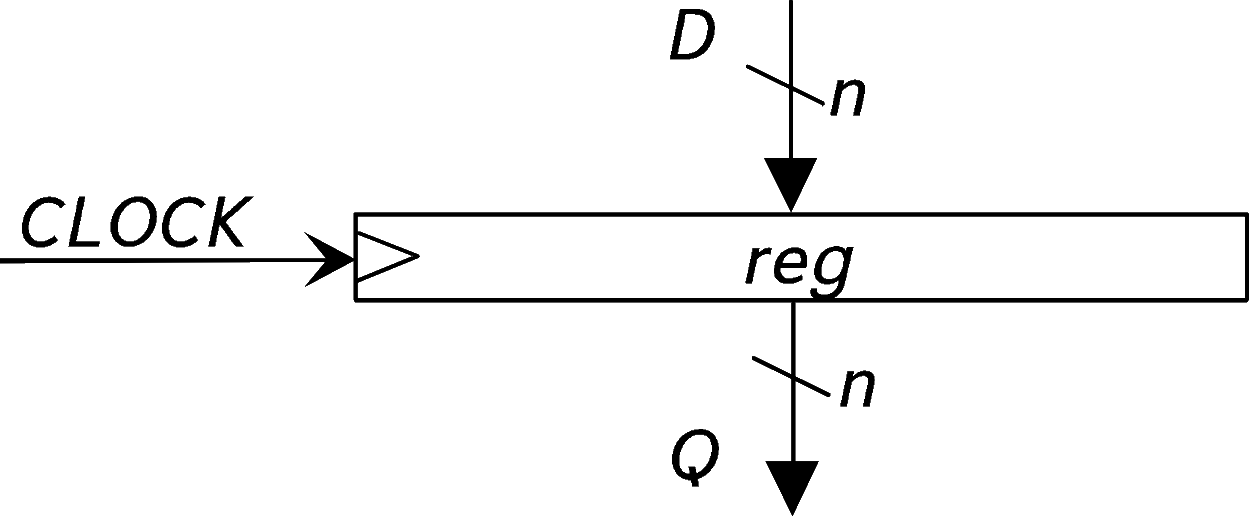
\includegraphics[width=0.50\textwidth]{figures/reg-pp}
  \end{center}
  \caption{Registro parallelo/parallelo}
\end{figure}


\begin{figure}[H]
  \begin{lstlisting}[language=Verilog]
    module RegistroParalleloParallelo #( parameter N = 8)(
      input [N-1:0] D,
      input clock,
      output [N-1:0] Q);
      reg [N-1:0] dato = 8'b00000000;
      assign Q = dato;
      always @(posedge clock) begin
        dato = D;
      end
    endmodule
  \end{lstlisting}
\end{figure}

\subsubsection{Registro seriale/seriale}
Memorizza i valori come sliding window e restituisce in output il valore più vecchio.
\begin{figure}[H]
  \begin{center}
    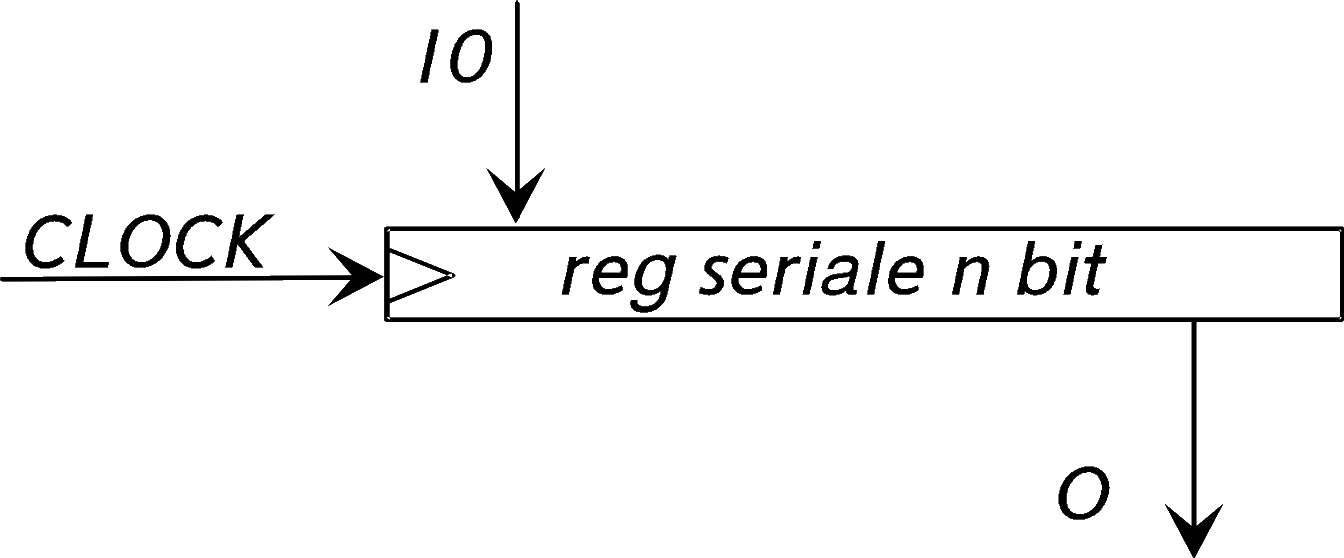
\includegraphics[width=0.50\textwidth]{figures/reg-ss}
  \end{center}
  \caption{Registro seriale/seriale}
\end{figure}

\begin{figure}[H]
  \begin{lstlisting}[language=Verilog]
    module RegistroSerialeSeriale (input I0, input clock,
      output O);
      parameter N = 8; reg [N-1:0] dato = 8'b00000000;
      assign O = dato[0];
      always @(posedge clock) begin
      dato = {I0, dato[N-1:1]};
        end
      endmodule
  \end{lstlisting}
\end{figure}

\subsubsection{Registro parallelo/seriale}
È un misto tra i 2 precedenti, ma con un valore che decide in che modo si comporta.
\begin{figure}[H]
  \begin{center}
    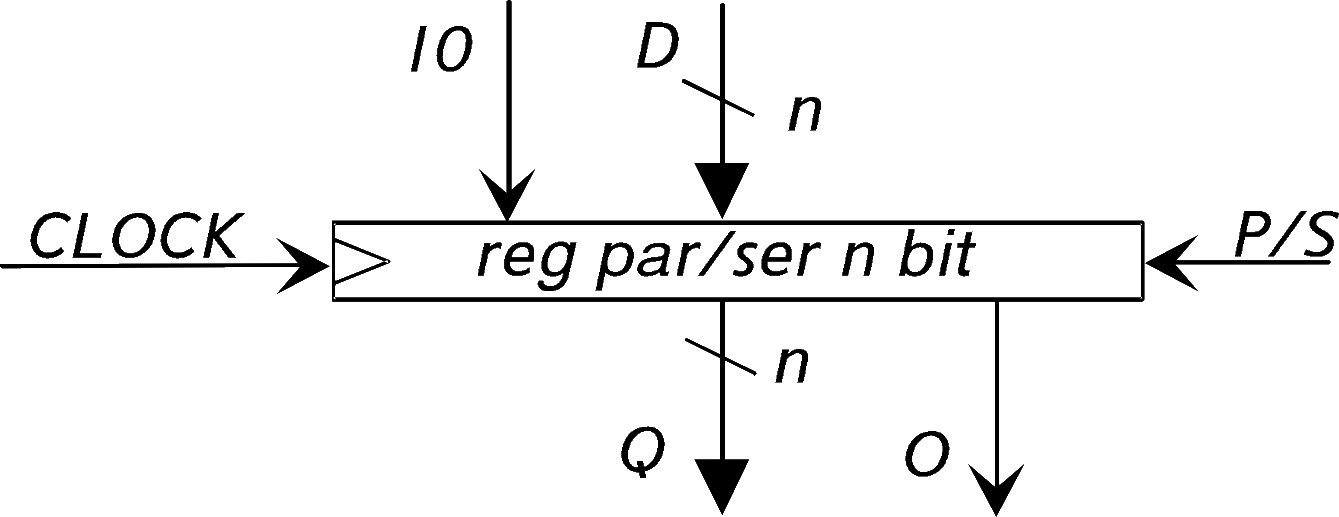
\includegraphics[width=0.50\textwidth]{figures/reg-ps}
  \end{center}
  \caption{Registro parallelo/seriale}
\end{figure}

\begin{figure}[H]
  \begin{lstlisting}[language=Verilog]
    module RegistroParalleloSeriale #(parameter N=8)(
      input PS, input I0, input [N-1:0] D, input clock,
      output [N-1:0] Q, output O);
      reg [N-1:0] dato = 8'b00000000;
      assign Q = dato;
      assign O = dato[0];
      always @(posedge clock) begin
        if(PS) dato = D;
        else dato = {I0, dato[N-1:1]};
      end
    endmodule
  \end{lstlisting}
\end{figure}

\subsection{Unità funzionali}
\subsubsection{Multiplexer}
Arrivano vari segnali e decido quale tenere.
\begin{figure}[H]
  \begin{center}
    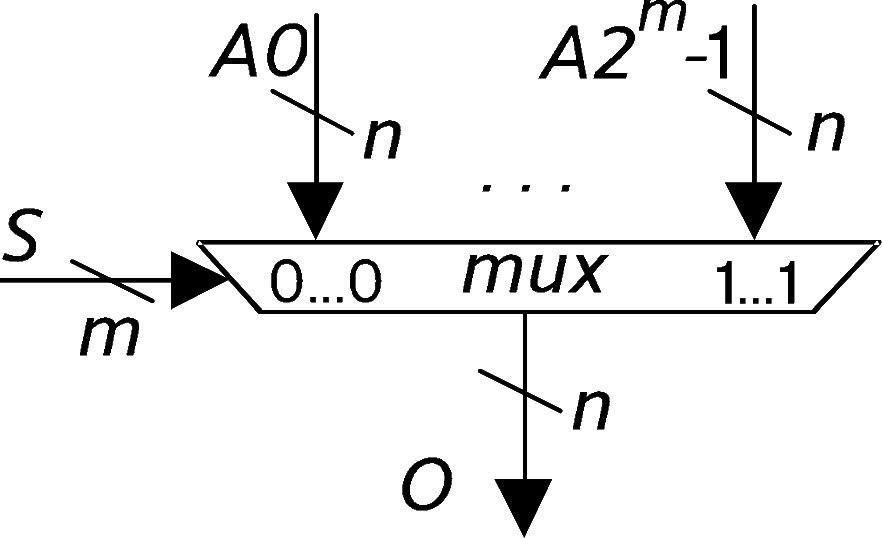
\includegraphics[width=0.40\textwidth]{figures/mux}
  \end{center}
  \caption{Multiplexer}
\end{figure}

\begin{figure}[H]
  \begin{lstlisting}[language=Verilog]
    module Multiplexer #(parameter N=8)(
      input [1:0] S, input [N-1:0] A3, input [N-1:0] A2,
      input [N-1:0] A1, input [N-1:0] A0,
      output reg [N-1:0] O);
      always @(A3, A2, A1, A0, S) begin
        case(S)
          2'b00: O = A0;
          2'b01: O = A1;
          2'b10: O = A2;
          2'b11: O = A3;
          default: O = 8'b00000000;
        endcase
      end
    endmodule
  \end{lstlisting}
\end{figure}

\subsubsection{Demultiplexer}
Arriva un segnale e decido dove mandarlo.
\begin{figure}[H]
  \begin{center}
    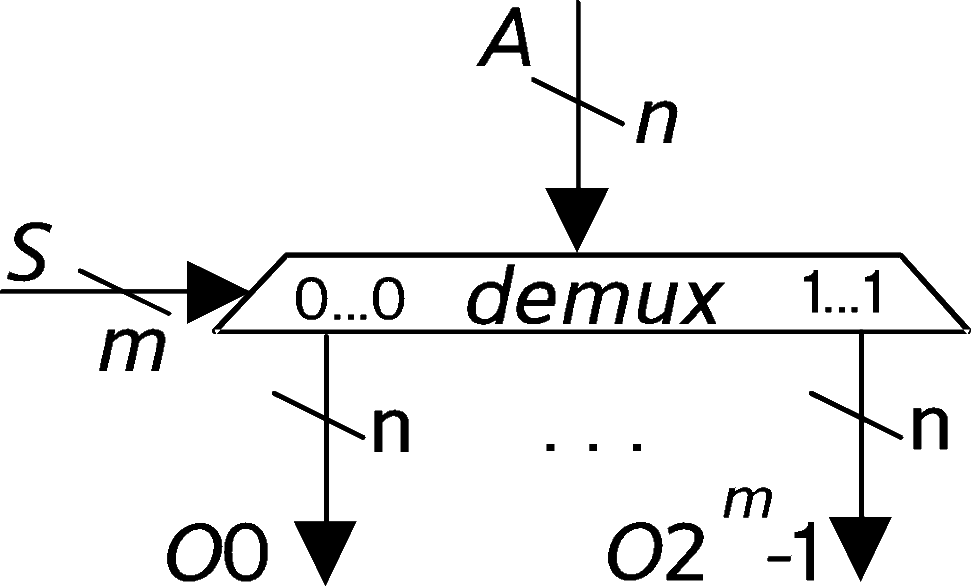
\includegraphics[width=0.40\textwidth]{figures/demux}
  \end{center}
  \caption{Demultiplexer}
\end{figure}

\begin{figure}[H]
  \begin{lstlisting}[language=Verilog]
    module Demultiplexer #(parameter N = 8) (
      input [1:0] S, input [N-1:0] A,
      output reg [N-1:0] O3, output reg [N-1:0] O2,
      output reg [N-1:0] O1, output reg [N-1:0] O0);
      
      always @(S,A) begin
        case(S)
          2'b00: begin
             O0 = A; O1 = 0; O2 = 0; O3 = 0;
           end
          2'b01: begin
             O0 = 0; O1 = A; O2 = 0; O3 = 0;
           end
          2'b10: begin
             O0 = 0; O1 = 0; O2 = A; O3 = 0;
           end
          2'b11: begin
             O0 = 0; O1 = 0; O2 = 0; O3 = A;
           end
        endcase
      end
    endmodule
  \end{lstlisting}
\end{figure}

\subsubsection{Decoder}
In uscita si ha un segnale che indica quale ingresso è attivo.
\begin{figure}[H]
  \begin{center}
    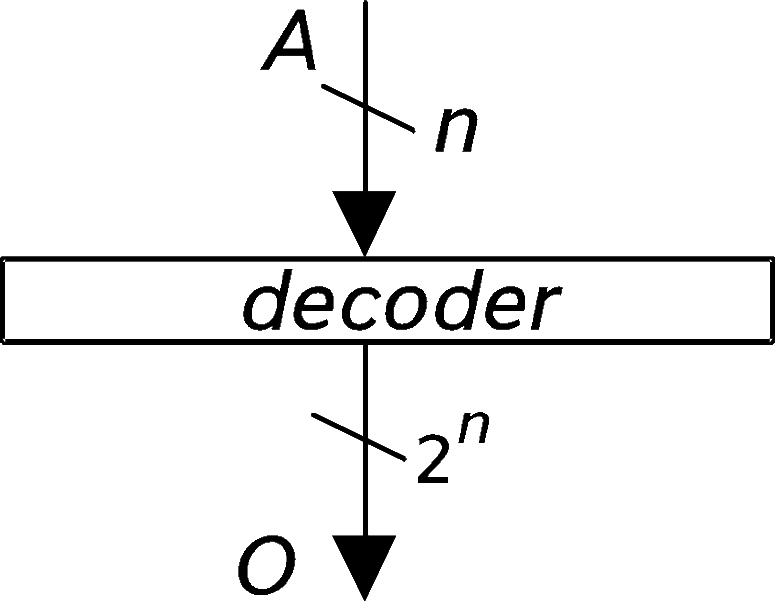
\includegraphics[width=0.25\textwidth]{figures/decoder}
  \end{center}
  \caption{Decoder}
\end{figure}

\begin{figure}[H]
  \begin{lstlisting}[language=Verilog]
    module Decoder #(parameter N = 8)(
      input [N-1:0] A, output reg [(2**N)-1:0] O);
      integer i;
      always @(A)
      begin
        for(i = 0; i < (2**N); i = i + 1) begin
          if(i == A) O[i] = 1'b1;
          else O[i] = 1'b0;
        end
      end
    endmodule
  \end{lstlisting}
\end{figure}

\subsubsection{Shifter}
Si inserisce un valore e si decide di quanto si vuole shiftare.
\begin{figure}[H]
  \begin{center}
    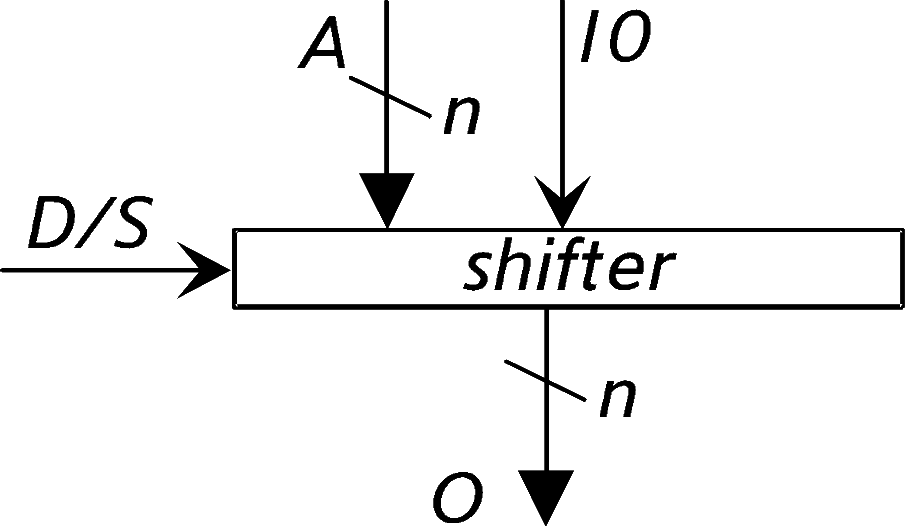
\includegraphics[width=0.40\textwidth]{figures/shifter}
  \end{center}
  \caption{Shifter}
\end{figure}

\begin{figure}[H]
  \begin{lstlisting}[language=Verilog]
    module Shifter #(parameter N = 8)
      (input DS, input [N-1:0] A, input I0,
      output reg [N-1:0] O);
      always @(A, I0) begin
      if(DS) O = {I0, A[N-1:1]};
      else O = {A[N-2:0], I0};
      end
    endmodule
  \end{lstlisting}
\end{figure}

\subsection{Unità aritmetiche}
\subsubsection{Sommatore}
Fa la somma tra 2 numeri in complemento a 2.
\begin{figure}[H]
  \begin{center}
    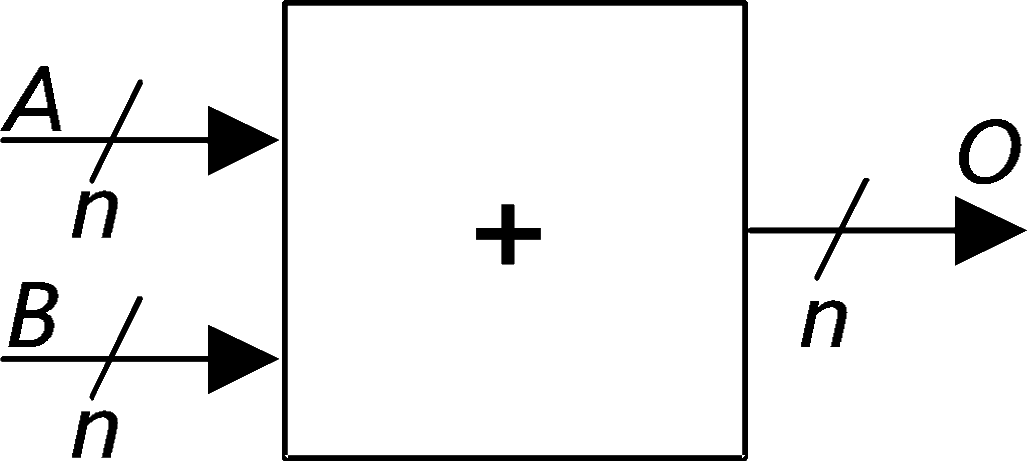
\includegraphics[width=0.40\textwidth]{figures/sum}
  \end{center}
  \caption{Sommatore}
\end{figure}

\begin{figure}[H]
  \begin{lstlisting}[language=Verilog]
    module Sommatore #(parameter N = 8)(
      input [N-1:0] A, input [N-1:0] B,
      output [N-1:0] O);
      assign O = A + B;
    endmodule
  \end{lstlisting}
\end{figure}


\subsubsection{Moltiplicatore}
Moltiplica 2 numeri in complemento a 2.
\begin{figure}[H]
  \begin{center}
    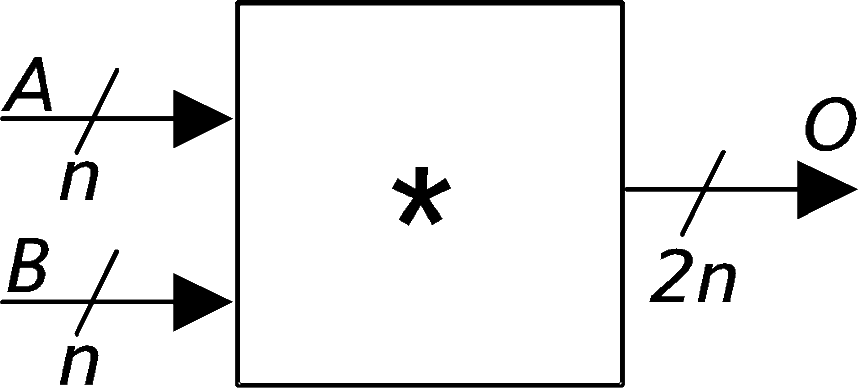
\includegraphics[width=0.40\textwidth]{figures/mul}
  \end{center}
  \caption{Moltiplicatore}
\end{figure}

\begin{figure}[H]
  \begin{lstlisting}[language=Verilog]
    module Moltiplicatore #(parameter N = 8)(
      input [N-1:0] A, input [N-1:0] B,
      output [(N**2)-1:0] O);
      assign O = A * B;
    endmodule
  \end{lstlisting}
\end{figure}


\subsection{Unità logiche}
\subsubsection{And}
Fa l'and tra 2 numeri nella stessa posizione, ad esempio: \( A_1 \wedge B_1 \ldots A_k \wedge B_k \) .
\begin{figure}[H]
  \begin{center}
    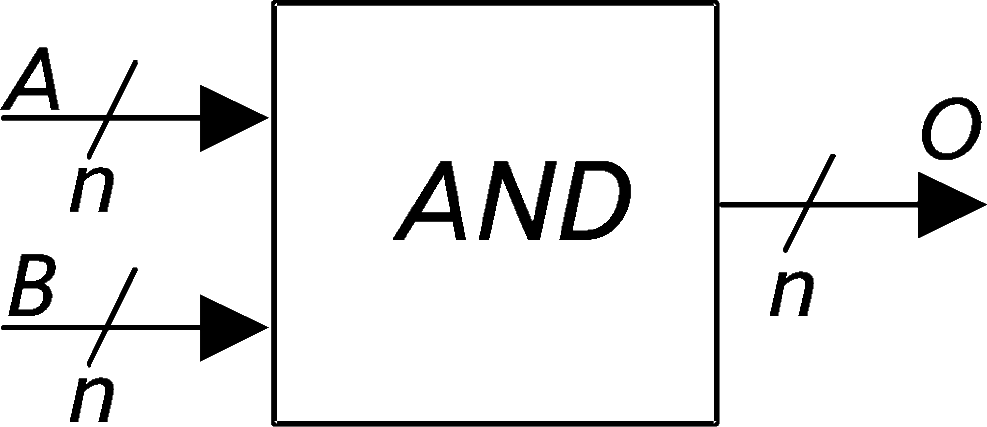
\includegraphics[width=0.40\textwidth]{figures/and}
  \end{center}
  \caption{And}
\end{figure}

\begin{figure}[H]
  \begin{lstlisting}[language=Verilog]
    module And #(parameter N = 8)(
      input [N-1:0] A, input [N-1:0] B,
      output reg [N-1:0] O);
        integer i;
        always @(A, B) begin
          for(i = 0; i < N; i = i + 1) begin
            O[i] = A[i] & B[i];
          end
        end
    endmodule
  \end{lstlisting}
\end{figure}

\subsubsection{Not}
Inverte i valori di un numero.
\begin{figure}[H]
  \begin{center}
    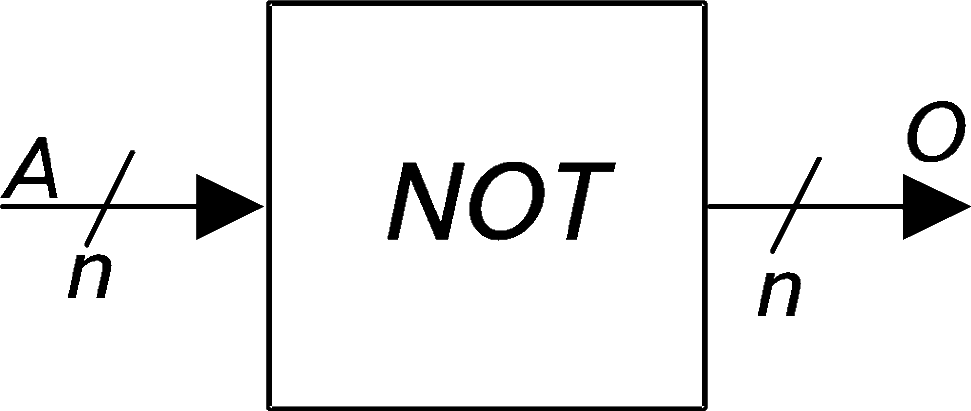
\includegraphics[width=0.40\textwidth]{figures/not}
  \end{center}
  \caption{Not}
\end{figure}

\begin{figure}[H]
  \begin{lstlisting}[language=Verilog]
    module Not #(parameter N = 8)(
      input [N-1:0] A
      output reg [N-1:0] O);
        integer i;
        always @(A) begin
          for(i = 0; i < N; i = i + 1) begin
            O[i] = ~A[i];
          end
        end
    endmodule
  \end{lstlisting}
\end{figure}

\subsubsection{Altri operatori logici}
\begin{itemize}
  \item Or
  \item Nand
  \item Nor
  \item Xor
  \item XNor
\end{itemize}

\subsection{Operatori di controllo}
\subsubsection{Maggiore}
\begin{figure}[H]
  \begin{center}
    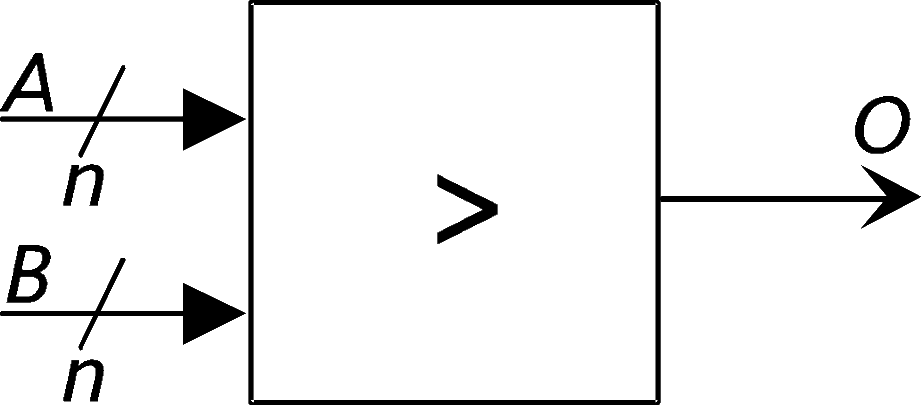
\includegraphics[width=0.40\textwidth]{figures/greater}
  \end{center}
  \caption{Maggiore}
\end{figure}

\begin{figure}[H]
  \begin{lstlisting}[language=Verilog]
    module Maggiore #(parameter N = 8)(
     input [N-1:0] A, input [N-1:0] B,
     output reg O);

       always @(A, B) begin
         if( A > B ) O = 1'b1;
         else O = 1'b0;
       end
    endmodule
  \end{lstlisting}
\end{figure}

\subsection{Esempio}
    Si vuole costruire un ALU da 8 bit (in complemento a 2) con accumulatore (registro che salva
    l'ultimo risultato calcolato) che esegue 4 operazioni:
    \begin{itemize}
      \item Somma
      \item Sottrazione
      \item Maggiore/Minore
    \end{itemize}

    Manca il componente del sottrattore, ma si può creare facilmente facendo la somma di
    un numero negativo. Si implementa quindi un componente che inverte un numero:
    \begin{figure}[H]
      \centering
        \begin{circuitikz}[square/.style={regular polygon,regular polygon sides=4}]
          \draw[-latex]
            (0,0) node[square,draw, minimum size=2cm, scale=0.7] (not) {NOT}
            (not.north) -- ++(0,1) node[above] {$A$}
            (0.5, -2) node[square,draw, minimum size=2cm, scale=0.7] (sum) {\huge$+$}
            (not.south) -- ++(0,-0.5) -- ++(0.35,0) to (0.35, -1.5);
          \draw[-latex] (0.7, 1.5) node[above right, xshift=-10] {\tiny$00000001$} to (0.7, -1.5)
            ;
          \draw[-latex] (sum.south) -- ++(0,-1);

          \draw (-0.1, 1) -- ++(0.2, 0.2) node[right] {\tiny 8};
          \draw (0.4, -3) -- ++(0.2, 0.2) node[right] {\tiny 8};

          \draw (0,1.35) -- ++(1.5,0) -- ++(0, -4.5) -- ++(-2.5,0) -- ++(0,4.5) -- (0,1.35);
          \end{circuitikz}
        \caption{Circuito invertitore}
     \end{figure}
     Questo circuito diventerà quindi un nuovo componente:
     \begin{figure}[H]
       \centering
         \begin{circuitikz}[square/.style={regular polygon,regular polygon sides=4}]
           \draw[-latex] (0,0) node[left] {A} -- ++(1,0) node[square,draw, minimum size=2cm, scale=0.7, xshift=20] (inv) {\huge $-$};
           \draw[-latex] (inv.east) -- ++(1,0) node[right] {O};

          \draw (0.4, -0.1) -- ++(0.2, 0.2) node[above] {\small n};
          \draw (2.4, -0.1) -- ++(0.2, 0.2) node[above] {\small n};
         \end{circuitikz}
     \end{figure}
    Un segnale di input "STORED" mi dice se usare "OP2" o un accumulatore
    \begin{figure}[H]
      \centering
        \begin{circuitikz}[square/.style={regular polygon,regular polygon sides=4}]
          % Multiplexer 2 to 1
          \draw (0,0) node (mux1-0) {0};
          \draw (0.5,0) node (mux1-1) {1};
          \draw (0.0,0.2) node (mux1-i0) {};
          \draw (0.5,0.2) node (mux1-i1) {};
          \draw (-0.3,0) node (mux1-s) {};
          \draw (0.25,-0.18) node (mux1-o) {};
          \draw (-0.5,0.3) -- ++(1.5,0) -- ++(-0.25, -0.6) -- ++(-1,0) -- ++(-0.25,0.6) -- (-0.5,0.3);
          % ------------------

          % Multiplexer2 2 to 1
          \draw (2,-3.6) node (mux2-0) {0};
          \draw (2.5,-3.6) node (mux2-1) {1};
          \draw (2,-3.4) node (mux2-i0) {};
          \draw (2.5,-3.4) node (mux2-i1) {};
          \draw (1.7,-3.6) node (mux2-s) {};
          \draw (2.25,-3.78) node (mux2-o) {};
          \draw (1.5,-3.3) -- ++(1.5,0) -- ++(-0.25, -0.6) -- ++(-1,0) -- ++(-0.25,0.6) -- cycle;
          % ------------------
          
          % Multiplexer3 2 to 1
          \draw (4.5,-3.6) node (mux3-0) {0};
          \draw (5,-3.6) node (mux3-1) {1};
          \draw (4.5,-3.4) node (mux3-i0) {};
          \draw (5,-3.4) node (mux3-i1) {};
          \draw (4.2,-3.6) node (mux3-s) {};
          \draw (4.75,-3.78) node (mux3-o) {};
          \draw (4,-3.3) -- ++(1.5,0) -- ++(-0.25, -0.6) -- ++(-1,0) -- ++(-0.25,0.6) -- cycle;
          % ------------------

          % Multiplexer 4 to 1
          \draw (-0.7,-6) node (mux4-0) {00};
          \draw (0,-6) node (mux4-1) {01};
          \draw (0.7,-6) node (mux4-2) {10};
          \draw (1.4,-6) node (mux4-3) {11};
          \draw (-0.7,-5.8) node (mux4-i0) {};
          \draw (0,-5.8) node (mux4-i1) {};
          \draw (0.7,-5.8) node (mux4-i2) {};
          \draw (1.4,-5.8) node (mux4-i3) {};
          \draw (-1.1,-6) node (mux4-s) {};
          \draw (0.25,-6.18) node (mux4-o) {};
          \draw (-1.3,-5.7) -- ++(3.3,0) -- ++(-0.25, -0.6) -- ++(-2.8,0) -- ++(-0.25,0.6) -- cycle;
          % ------------------

          % Register
          \draw (2,1.3) node[rectangle ,draw, minimum width=2cm, minimum height=0.7cm, scale=0.7] (reg) {REG};
          \draw (reg.east) -- ++(0,0.15) -- ++(-0.2, -0.15) -- ++(0.2,-0.15);
          \draw[latex-] (reg.east) -- ++(0.5,0) node[below] {\tiny CLK};
          % ------------------


          % Operators
          \draw (3.5,-2) node[square,draw, minimum size=2cm, scale=0.6] (lesser) {\huge$<$};
          \draw (1,-2) node[square,draw, minimum size=2cm, scale=0.6] (greater) {\huge$>$};
          \draw (-1.5,-3.5) node[square,draw, minimum size=2cm, scale=0.6] (sum2) {\huge$+$};
          \draw (-1,-2) node[square,draw, minimum size=2cm, scale=0.6] (sub) {\huge$-$};
          \draw (-3,-2) node[square,draw, minimum size=2cm, scale=0.6] (sum1) {\huge$+$};
          % ------------------

          \draw[latex-] (mux1-i0) -- ++(0,1) node[above] {\small OP2};
          \draw[latex-] (mux1-s) -- ++(-1,0) -- ++(0,1.2) node[above] {\small STORED};
          \draw[latex-] (mux1-i1) -- ++(0,0.5) -- ++(1.5,0) -- (reg.south);

          % OP1
          \draw[latex-] (-3.2, 52 |- sum1.north) -- ++(0,2.8) node[above] (OP1) {\small OP1};

          \draw[-latex] (mux1-o) -- ++(0,-1) to[short, *-] ++(3.5,0) to[short, *-] ++(0,-0.39);
          \draw[-latex] (mux1-o) -- ++(0,-1) to[short] ++(1,0) to[short, *-] ++(0,-0.39);
          \draw[-latex] (mux1-o) -- ++(0,-1) to[short] ++(-1,0) to[short, *-] ++(0,-0.39);
          \draw[-latex] (mux1-o) -- ++(0,-1) to[short] ++(-3,0) to[short, *-] ++(0,-0.39);
          \draw[-latex] (mux1-o) -- ++(0,-1) to[short] (mux2-i1 |- 52,-1.18) to[short, *-] (mux2-i1);
          \draw[-latex] (mux1-o) -- ++(0,-1) to[short] (mux3-i1 |- 52,-1.18) to[short, *-] (mux3-i1);

          \draw[-latex] (sub.south) -- ++(0,-0.25) -- ++(-0.25,0) -- ++(0,-0.4);
          \draw[-latex] (greater.south) |- (mux2-s);
          \draw[-latex] (lesser.south) |- (mux3-s);

          \draw[-latex] (OP1) -- ++(0, -2.2) to[short, *-] ++(2,0) to[short, *-] (-1.2, 52 |- sub.north);
          \draw[-latex] (OP1) -- ++(0, -2.2) to[short, *-] ++(1.5,0) to[short, *-] (-1.7, 52 |- sum2.north);
          \draw[-latex] (OP1) -- ++(0, -2.2) to[short] ++(4,0) to[short, *-] (0.8, 52 |- greater.north);
          \draw[-latex] (OP1) -- ++(0, -2.2) to[short] ++(6.5,0) to[short, *-] (3.3, 52 |- lesser.north);
          \draw[-latex] (OP1) -- ++(0, -2.2) to[short] (mux2-i0 |- 52,-0.74) to[short, *-] (mux2-i0);
          \draw[-latex] (OP1) -- ++(0, -2.2) to[short] (mux3-i0 |- 52,-0.74) to[short, *-] (mux3-i0);

          \draw[-latex] (sum1.south) -- ++(0,-2.5) |- (mux4-i0 |- 52,-5) -- (mux4-i0);
          \draw[-latex] (sum2.south) -- ++(0,-0.5) -- ++(1.5,0) |- (mux4-i1 |- 52,-5) -- (mux4-i1);
          \draw[-latex] (mux2-o) -- ++(0,-0.65) -- ++(-1.55,0) |- (mux4-i2 |- 52,-5) -- (mux4-i2);
          \draw[-latex] (mux3-o) -- ++(0,-1.22) -- ++(-3.1,0) |- (mux4-i3 |- 52,-5) -- (mux4-i3);
 
          \draw[-latex] (mux4-o) -- ++(0,-0.5) -- ++(5.8,0) -- ++(0,8.5) |- (reg.north |- 52,2) -- (reg.north);

          \draw[latex-] (mux4-s) -- ++(-3,0) -- ++(0,7.23) node[above] {\small OP};

          % Bit numbers
          % OP2
          \draw (-0.1, 0.9) -- ++(0.2, 0.2) node[right, yshift=-2] {\tiny 8};
          % STORED 
          \draw (-1.4, 0.9) -- ++(0.2, 0.2) node[right, yshift=-2] {\tiny 1};
          % OP1
          \draw (-3.3, 0.9) -- ++(0.2, 0.2) node[right, yshift=-2] {\tiny 8};
          % OP
          \draw (-4.2, 0.9) -- ++(0.2, 0.2) node[right, yshift=-2] {\tiny 2};
          % mux1
          \draw (0.15, -0.6) -- ++(0.2, 0.2) node[right, yshift=-2] {\tiny 8 SEL};
          % reg
          \draw (1.9, 0.8) -- ++(0.2, 0.2) node[right, yshift=-2] {\tiny 8};
          % mux2
          \draw (2.15, -4.2) -- ++(0.2, 0.2) node[right, yshift=-2] {\tiny 8};
          % mux3
          \draw (4.65, -4.2) -- ++(0.2, 0.2) node[right, yshift=-2] {\tiny 8};
          % mux4
          \draw (0.15, -6.6) -- ++(0.2, 0.2) node[right, yshift=-2] {\tiny 8};
          % greater
          \draw (0.9, -2.7) -- ++(0.2, 0.2) node[right, yshift=-2] {\tiny 1};
          % lesser
          \draw (3.4, -2.7) -- ++(0.2, 0.2) node[right, yshift=-2] {\tiny 1};
          % sum1
          \draw (-3.1, -2.7) -- ++(0.2, 0.2) node[right, yshift=-2] {\tiny 8};
          % sub
          \draw (-1.07, -2.64) -- ++(0.15, 0.15) node[right, yshift=-2] {\tiny 8};
          % sum2
          \draw (-1.6, -4.2) -- ++(0.2, 0.2) node[right, yshift=-2] {\tiny 8};
          % ------------------

        \end{circuitikz}
    \end{figure}
    Il codice del circuito è il seguente:
    \begin{figure}[H]
      \begin{lstlisting}[language=Verilog]
        module Opposto #(parameter N = 8)(
          input [N-1:0] operando,
          output [N-1:0] risultato);
            assign risultato = -operando;
        endmodule
      \end{lstlisting}
    \end{figure}

    \begin{figure}[H]
      \begin{lstlisting}[language=Verilog]
        module ALU #(parameter N = 8)(
          input clock,
          input [N-1:0] op1,
          input [N-1:0] op2,
          input stored,
          input [1:0] oper,
          output [N-1:0] O);
          
            wire [N-1:0] acc, sel, t1, t2, t3, t4, t5, out;
            wire s1, s2;

            RegistroParalleloParallelo registro(out, clock, acc);
            Multiplexer2 mux1(stored, acc, op2, sel);
            Multiplexer2 mux2(s1, op1, sel, t3);
            Multiplexer2 mux3(s2, op1, sel, t4);
            Multiplexer mux4(oper, t4, t3, t2, t1, out);
            Sommatore sum1(op1, sel, t1);
            Opposto opp1(sel, t5);
            Sommatore sum2(op1, t5, t2);
            Maggiore mag(op1, sel, s1);
            Minore min(op1, sel, s2);

            assign O = out;
        endmodule
      \end{lstlisting}
    \end{figure}

    Di seguito il codice implementato con il metodo Behavioural:
    \begin{figure}[H]
      \begin{lstlisting}[language=Verilog]
        module ALU_behav #(parameter N = 8)(
          input clock,
          input [N-1:0] op1,
          input [N-1:0] op2,
          input stored,
          input [1:0] oper,
          output [N-1:0] O);

            reg [N-1:0] acc, sel, out;

            always @(stored, acc, op2) begin
              if(stored) sel = acc;
              else sel = op2;
            end

            always @(posedge clock) begin
              if(clock) acc = out;
            end

            assign O = out;

            always @(op1, sel, oper) begin
              case(oper)
              2'b00 :
                out = op1 + sel;
              2'b01 :
                out = op1 - sel;
              2'b10 :
                if(op1 > sel) out = op1;
                else out = sel;
              2'b11 :
                if(op1 < sel) out = op1;
                else out = sel;
              endcase
            end
        endmodule
      \end{lstlisting}
    \end{figure}

\section{Modello FSMD (FSM con Datapath o Controllore/Datapath)}
È composto da 2 parti:
\begin{itemize}
  \item \textbf{Controllo}: Finite State Machine
  \item \textbf{Elaborazione}: Datapath
\end{itemize}
\begin{figure}[H]
  \begin{center}
    \begin{tikzpicture}
      \draw (0,0) rectangle (2,2) node[pos=.5] {FSM};
      \draw[->] (1,0) -- (1,-1) node[below, align=center, scale=0.8] {Uscite di\\ controllo};
      \draw[<-] (1,2) -- (1,3) node[above, align=center, scale=0.8] {Ingressi di\\ controllo};

      \draw (4,0) rectangle (6,2) node[pos=.5] {Datapath};
      \node[draw, single arrow,
              minimum height=10mm, minimum width=8mm,
              single arrow head extend=2mm,
              anchor=west, rotate=-90] at (5,0) {};
      \node[draw, single arrow,
              minimum height=10mm, minimum width=8mm,
              single arrow head extend=2mm,
              anchor=west, rotate=-90] at (5,3) {};
      \node at (5,-1) [below, align=center, scale=0.8] {Risultati};
      \node at (5,3) [above, align=center, scale=0.8] {Dati in\\ingresso};

      \draw[->] (4,1.5) -- (2,1.5) node[pos=.5, above, align=center, scale=0.8] {Segnali di\\ stato};
      \draw[<-] (4,0.5) -- (2,0.5) node[pos=.5, below, align=center, scale=0.8] {Segnali di\\ controllo};

      \draw[<-] (0.5,0) -- ++(0,-0.5) -- ++(-1,0) node[left, align=center, scale=0.8] {CLK};
      \draw[fill] (0.5,-0.5) circle (0.05);
      \draw[->] (0.5,-0.5) -- (4.5, -0.5) -- ++(0,0.5);

      \draw (6.5,3) -- ++(0.3,0) -- ++(0,-1) node[right, yshift=15, align=center] {Primary\\input} -- ++(-0.3,0);
      \draw (6.5,0) -- ++(0.3,0) -- ++(0,-1) node[right, yshift=15, align=center] {Primary\\output} -- ++(-0.3,0);
    \end{tikzpicture}
  \end{center}
  \caption{Modello FSMD}
\end{figure}
Per progettare il modello precedente servono diversi passaggi:
\begin{enumerate}
  \item Definire l'insieme di operazioni necessarie (identificare le unità funzionali necessarie)
  \item Identificare le operazioni che le unità funzionali devono svolgere 
  \item Identificare le necessità di memorizzare i dati (ad esempio i risultati intermedi)
  \item Progetto il datapath di ogni operazione
  \item Identificare i segnali di controllo
  \item Progettare il controllore (FSM) che genera i segnali di controllo
\end{enumerate}
Questi passi non danno sempre una decisione univoca, infatti si possono prendere più decisioni
che permettono di bilanciare il modello per avere una parte preponderante di macchina a stati,
oppure una parte preponderante di datapath.
\subsection{Esempio}
    Prendiamo in considerazione l'esempio del semaforo:

    Per evitare incidenti, il circuito di controllo deve garantire che le luci sulle
    strade NS e EO siano sempre accese in opposizione. Il circuito assegna
    priorità alla strada NS e commuta dal verde al rosso su NS solo se
    TRAFFICONS=0 e TRAFFICOEO=1, in caso contrario mantiene il verde
    su NS. In assenza di traffico sia su NS che su EO il semaforo non modifica
    la configurazione raggiunta. Non appena giunge traffico su NS,
    indipendentemente da cosa succede su EO, il semaforo assegna la luce
    verde a NS e la luce rossa a EO.

    Gli input sono:
    \begin{itemize}
      \item \textbf{TRAFFICONS[1]}: 1 indica traffico su nord-sud
      \item \textbf{TRAFFICOEO[1]}: 1 indica traffico su est-ovest
    \end{itemize}

    Le uscite sono:
    \begin{itemize}
      \item \textbf{LUCENS[1]}: 1 indica luce verde su nord-sud
      \item \textbf{LUCENEO[1]}: 1 indica luce verde su est-ovest
    \end{itemize}
\begin{figure}[H]
  \begin{center}
    \begin{tikzpicture}[node distance=4cm and 2cm,>=stealth',auto, every place/.style={draw}]
      \node [place] (A) [scale=0.7] {VERDENS};
      \coordinate[node distance=1.3cm,left of=A] (left-A);
      \coordinate[node distance=1.3cm,right of=A] (right-A);

      \node [place] (B) [right of= A, scale=0.7] {VERDEEO};


      \path[->] (A) edge [loop left] node[xshift=2,scale=0.9] {-0/10} ();

      \path[<-] (A) edge [bend left=20] node[scale=0.9] {1-/10} (B);
      \path[<-] (B) edge [bend left=20] node[scale=0.9] {01/01} (A);
      \path[->] (B) edge [loop right] node[xshift=-2,scale=0.9] {0-/01} ();
    \end{tikzpicture}
  \end{center}
  \caption{FSM del semaforo}
\end{figure}
    Aggiungiamo la funzionalità che il controllore non commuta mai da verde a rosso senza aver
    prima atteso 1024 cicli di clock.
        \begin{figure}[H]
      \centering
        \begin{circuitikz}[square/.style={regular polygon,regular polygon sides=4}, scale=1.3, transform shape]
          % Multiplexer 2 to 1
          \draw (0,0) node (mux1-0) {0};
          \draw (0.5,0) node (mux1-1) {1};
          \draw (0.0,0.2) node (mux1-i0) {};
          \draw (0.5,0.2) node (mux1-i1) {};
          \draw (-0.3,0) node (mux1-s) {};
          \draw (0.25,-0.18) node (mux1-o) {};
          \draw (-0.5,0.3) -- ++(1.5,0) -- ++(-0.25, -0.6) -- ++(-1,0) -- ++(-0.25,0.6) -- (-0.5,0.3);
          % ------------------


          % Register
          \draw (0.25,-1) node[rectangle ,draw, minimum width=2cm, minimum height=0.7cm, scale=0.7] (reg) {REG};
          \draw (reg.west) -- ++(0,0.15) -- ++(0.2, -0.15) -- ++(-0.2,-0.15);
          % ------------------

          % Operators
          \draw (1.2,-2.5) node[square,draw, minimum size=2cm, scale=0.6] (sum) {\huge$+$};
          \node[xshift=-5, yshift=-3] at (sum.north) (sum-i0) {};
          \node[xshift=5, yshift=-3] at (sum.north) (sum-i1) {};

          \draw (-0.75,-2.5) node[square,draw, minimum size=2cm, scale=0.6] (equiv) {\huge$=$};
          \node[xshift=-5, yshift=-3] at (equiv.north) (equiv-i0) {};
          \node[xshift=5, yshift=-3] at (equiv.north) (equiv-i1) {};
          % ------------------

          \draw[latex-] (mux1-i0) -- ++(0,1) node[above left, xshift=7] {\tiny 0000000000};
          \draw[latex-] (mux1-s) -- ++(-1,0) node[left, align=center, scale=0.8] {Inizio};

          \draw[-latex] (mux1-o) -- (reg.north);

          \draw[-latex] (reg.south) to[short] ++(0,-0.2) -| (sum-i0);
          \draw[-latex] (reg.south) to[short] ++(0,-0.2) -| (equiv-i0);

          \draw[latex-] (sum-i1) -- ++(0,0.8) node[above right, xshift=-7] {\tiny 0000000001};
          \draw[latex-] (equiv-i1) -- ++(0,0.4) node[above right, xshift=-7] {\tiny 1111111111};

          \draw[-latex] (equiv.south) -- ++(0,-0.5) -- ++(-1,0) node[left, align=center, scale=0.8] {Fine};
          \draw[-latex] (sum.south) -- ++(0,-0.5) -- ++(1.7,0) -- ++(0,4.5) -| (mux1-i1);

        \end{circuitikz}
        \caption{Datapath del contatore 1024}
    \end{figure}
\begin{figure}[H]
  \begin{center}
    \begin{tikzpicture}[node distance=4cm and 2cm,>=stealth',auto, every place/.style={draw}]
      \node [place] (A) [scale=0.7] {VERDENS};
      \coordinate[node distance=1.3cm,left of=A] (left-A);
      \coordinate[node distance=1.3cm,right of=A] (right-A);

      \node [place] (B) [below of= A, align=center, scale=0.7] {INIZIO\\ CONTO};
      \node [place] (C) [right of= B, scale=0.7] {VERDEEO};
      \node [place] (D) [above of= C, align=center, scale=0.7] {CONTO 2};


      \path[->] (A) edge [loop left] node[xshift=2,scale=0.9, align=center] {00-/100\\
        10-/100\\
        11-/100 } ();

      \path[<-] (A) edge [bend left=20] node[scale=0.9, align=center] {01-/101} (B);
      \path[<-] (B) edge [bend left=20] node[scale=0.9, align=center] {1--/100} (A);
      \path[->] (B) edge [loop left] node[xshift=-2,scale=0.9] {0-0/100} ();
      \path[->] (B) edge [bend right=20] node[scale=0.9, align=center] {011/010\\001/010} (C);
      \path[->] (C) edge [loop right] node[xshift=-2,scale=0.9] {0--/010} ();
      \path[->] (C) edge [bend right=20] node[scale=0.9, align=center] {1--/011} (D);
      \path[->] (D) edge [loop right] node[xshift=-2,scale=0.9] {--0/010} ();
      \path[->] (D) edge [bend right=20] node[scale=0.9, align=center] {--1/100} (A);
    \end{tikzpicture}
  \end{center}
  \caption{FSM del semaforo}
\end{figure}
\begin{figure}[H]
  \begin{center}
    \begin{tikzpicture}
      \draw (0,0) rectangle (2,2) node[pos=.5] {FSM};
      \draw[<-] (0.5,2) -- (0.5,3) node[above, align=center, scale=0.8, xshift=-10] {TrafficoNS};
      \draw[<-] (1.5,2) -- (1.5,3) node[above, align=center, scale=0.8, xshift=10] {TrafficoEO};

      \draw[->] (0.5,0) -- (0.5,-1) node[below, align=center, scale=0.8, xshift=-10] {LuceNS};
      \draw[->] (1.5,0) -- (1.5,-1) node[below, align=center, scale=0.8, xshift=10] {LuceEO};

      \draw (4,0) rectangle (6,2) node[pos=.5] {Datapath};

      \draw[<-] (4,1.5) -- (2,1.5) node[pos=.5, above, align=center, scale=0.8] {Inizio};
      \draw[->] (4,0.5) -- (2,0.5) node[pos=.5, below, align=center, scale=0.8] {Fine};

      \draw[<-] (0,0.5) -- ++(-0.5,0) -- ++(0,-1) -- ++(-1,0) node[left, align=center, scale=0.8] {CLK};
      \draw[fill] (-0.5,-0.5) circle (0.05);
      \draw[->] (-0.5,-0.5) -- (4.5, -0.5) -- ++(0,0.5);

      \draw (3.5, 1.4) -- ++(0.2, 0.2) node[below, yshift=-2] {\tiny 1};
      \draw (3.5, 0.4) -- ++(0.2, 0.2) node[below, yshift=-2] {\tiny 1};
    \end{tikzpicture}
  \end{center}
  \caption{Modello FSMD del semaforo}
\end{figure}
L'implementazione in Verilog è la seguente:
\begin{figure}[H]
  \begin{lstlisting}[language=Verilog]
  module SemaforoTemporizzato(
    input rst, clk, trafficons, trafficoeo,
    output reg lucens, luceeo);
    
    reg [1:0] stato = 2'b00;
    reg [1:0] stato_prossimo = 2'b00;
    reg inizio = 1'b0, fine = 1'b0;
    reg [3:0] registro = 3'b000;

    always @(clk) begin : UPDATE
      if(rst) stato = 2'b00;
      else stato = stato_prossimo;
    end

    always @(clk) begin : DATAPATH
      if(inizio) begin
        registro = 3'b000;
        fine = 1'b0;
      end else begin

      if(registro < 3'b111) begin
        registro = registro + 1'b1;
        fine = 1'b0;
      end
      else begin
        fine = 1'b1;
      end
    end
    ...
  \end{lstlisting}
\end{figure}

\begin{figure}[H]
  \begin{lstlisting}[language=Verilog]
    ...
    always @(stato, trafficons, trafficoeo, fine) begin : FSM
      case(stato)
      2'b00:
        if(~trafficons && trafficoeo) begin
          lucens = 1'b1; luceeo = 1'b0; inizio = 1'b1;
          stato_prossimo = 2'b10;
        end else begin
          lucens = 1'b1; luceeo = 1'b0;
          stato_prossimo = 2'b00;
        end
      2'b01:
        if(~trafficons) begin
          lucens = 1'b0; luceeo = 1'b1;
          stato_prossimo = 2'b01;
        end else begin
          lucens = 1'b0; luceeo = 1'b1; inizio = 1'b1;
          stato_prossimo = 2'b11;
        end
      2'b10:
        begin inizio = 1'b0;
        if(trafficons) begin
          lucens = 1'b1; luceeo = 1'b0;
          stato_prossimo = 2'b00;
        end
        else if(fine) begin
          lucens = 1'b0; luceeo = 1'b1;
          stato_prossimo = 2'b01;
        end else begin
          lucens = 1'b1; luceeo = 1'b0;
          stato_prossimo = 2'b10;
        end end
      2'b11:
        begin inizio = 1'b0;
        if(fine) begin
          lucens = 1'b1; luceeo = 1'b0;
          stato_prossimo = 2'b00;
        end else begin
          lucens = 1'b0; luceeo = 1'b1;
          stato_prossimo = 2'b11;
        end end
      endcase
    end
  end
  \end{lstlisting}
\end{figure}

\section{High Level Synthesis}
Verrà fatto vedere in C come si può scrivere un codice che verrà poi sintetizzato in VHDL. Implementiamo
l'algoritmo per calcolare il massimo comune divisore:
\begin{figure}[H]
  \begin{center}
    \begin{circuitikz}[square/.style={regular polygon,regular polygon sides=4}]
      \draw (0,0) node[square,draw, minimum size=2cm, scale=0.6] (gcd) {\huge GCD};
      \draw[latex-] (-0.8,0.3) -- ++(-0.8,0) node[left] {x};
      \draw[latex-] (-0.8,-0.3) -- ++(-0.8,0) node[left] {y};
      \draw[-latex] (0.8,-0.3) -- ++(0.8,0) node[right] {out};
      \draw[-latex] (0.8,0.3) -- ++(0.8,0) node[right] {done};
    \end{circuitikz}
  \end{center}
  \caption{Circuito per il calcolo del massimo comune divisore}
\end{figure}
Bisogna indicare al circuito quando il risultato è giusto, quindi si aggiunge un segnale di controllo
per indicare che il risultato è pronto e la chiamo \textbf{done}.

\vspace{1em}
Il codice in C è il seguente:
\begin{figure}[H]
  \begin{lstlisting}[language=C]
    int gcd(int x, int y) {
      int temp;
      while(x > 0) {
        if(y <= x) { // Si mette y <= x per poter riutilizzare lo stesso componente del > ma negato
          temp = x;
          x = y;
          y = temp;
        }
        x = x - y;
      }
      return y;
    }
  \end{lstlisting}
\end{figure}
\begin{figure}[H]
  \begin{center}
    \begin{tikzpicture}
      \draw (0,0) rectangle (2,2) node[pos=.5] {FSM};

      \draw[-latex] (3,4) -- ++(0,-1) -| (1,2);
      \draw[-latex] (3,3) -| (5,2);

      \draw (1,0) |- (3,-1.5);
      \draw (5,0) |- (3,-1.5);
      \draw[-latex] (3,-1.5) -- ++(0,-1);

      \draw (4,0) rectangle (6,2) node[pos=.5] {Datapath};

      \draw[<-] (4,1.5) -- (2,1.5) node[pos=.5, above, align=center, scale=0.8] {};
      \draw[->] (4,0.5) -- (2,0.5) node[pos=.5, below, align=center, scale=0.8] {};

      \draw[<-] (0,0.5) -- ++(-0.5,0) -- ++(0,-1) -- ++(-1,0) node[left, align=center, scale=0.8] {CLK};
      \draw[fill] (-0.5,-0.5) circle (0.05);
      \draw[->] (-0.5,-0.5) -- (4.5, -0.5) -- ++(0,0.5);

    \end{tikzpicture}
  \end{center}
  \caption{Modello del progetto a cui si vuole arrivare}
\end{figure}

\begin{itemize}
  \item \textbf{Scheduling}: si decide in che cicli di clock effettuare le operazioni
  \item \textbf{Allocation}: si decide dove allocare le operazioni
\end{itemize}


\begin{figure}[H]
  \begin{center}
    \begin{tikzpicture}[node distance=3cm and 2cm,>=stealth',auto, every place/.style={draw}]
      \node [place] (Init) {Init};
      \coordinate[node distance=1.3cm,left of=Init] (left-Init);
      \coordinate[node distance=1.3cm,right of=Init] (right-Init);

      \node [place] (While) [right of= Init, align=center, scale=0.8] {While};
      \node [place] (If) [below of= While] {If};
      \node [place] (EndIf) [left of= If, align=center, scale=0.7] {End\\if};
      \node [place] (End) [right of= While, align=center] {End};

      \path[->] (Init) edge [bend left=20] node[scale=0.9, align=center] {/read x\\/read y} (While);
      \path[->] (While) edge [bend left=20] node[scale=0.9, align=center] {$x>0$/} (If);
      \path[->] (While) edge [bend left=20] node[scale=0.9, align=center] {$x \le 0/out=y$\\$x \le 0 / done = 1$} (End);
      \path[->] (If) edge [bend left=20] node[scale=0.9, align=center] {$y>x/temp = x$\\
        $y > x /x = y$\\$y > x/ y = temp$} (EndIf);
      \path[->] (If) edge [bend right=20] node[scale=0.9, align=center] {$x \le y$} (EndIf);
      \path[->] (EndIf) edge node[scale=0.9, align=center] {/x = x - y} (While);
    \end{tikzpicture}
  \end{center}
  \caption{FSM annotata}
\end{figure}
Ad esempio con 8 cicli di clock si produce il risultato se \( x = 8 \) e \( y = 4 \). Per capire
quali sono i registri necessari dalla FSM si controlla quali sono le variabili che vengono assegnate
in un ciclo di clock e vengono utilizzate in un ciclo di clock diverso, in quel caso si utilizza
un registro. In questo caso si utilizzano 2 registri, uno per \( x \) e uno per \( y \), \( temp \) 
è soltanto un filo perchè viene usato soltanto in un cilclo di clock.

\vspace{1em}
Per implementare il circuito controllore si utilizzano le condizioni definite
nel diagramma di stato. Si aggiunge un segnale di controllo per ogni condizione:
\begin{figure}[H]
  \centering
    \begin{circuitikz}[square/.style={regular polygon,regular polygon sides=4}, scale=1.3, transform shape]
      % Multiplexer 6 to 1
      \draw (-1,0.2) node (mux1-i1) {};
      \node at (mux1-i1) [below, scale=0.7, yshift=-1] {001};
      \draw (-0.5,0.2) node (mux1-i2) {};
      \node at (mux1-i2) [below, scale=0.7, yshift=-1] {010};
      \draw (0.0,0.2) node (mux1-i3) {};
      \node at (mux1-i3) [below, scale=0.7, yshift=-1] {011};
      \draw (0.5,0.2) node (mux1-i4) {};
      \node at (mux1-i4) [below, scale=0.7, yshift=-1] {100};
      \draw (1.0,0.2) node (mux1-i5) {};
      \node at (mux1-i5) [below, scale=0.7, yshift=-1] {101};
      \draw (1.5,0.2) node (mux1-i6) {};
      \node at (mux1-i6) [below, scale=0.7, yshift=-1] {110};

      \draw (-1.3,0) node (mux1-s) {};
      \draw (0.25,-0.18) node (mux1-o) {};

      \draw (-1.5,0.3) -- ++(3.5,0) -- ++(-0.25, -0.6) -- ++(-3,0) -- ++(-0.25,0.6) -- cycle;
      % ------------------

      % Multiplexer2 6 to 1
      \draw (3,0.2) node (mux2-i1) {};
      \node at (mux2-i1) [below, scale=0.7, yshift=-1] {001};
      \draw (3.5,0.2) node (mux2-i2) {};
      \node at (mux2-i2) [below, scale=0.7, yshift=-1] {010};
      \draw (4,0.2) node (mux2-i3) {};
      \node at (mux2-i3) [below, scale=0.7, yshift=-1] {011};
      \draw (4.5,0.2) node (mux2-i4) {};
      \node at (mux2-i4) [below, scale=0.7, yshift=-1] {100};
      \draw (5,0.2) node (mux2-i5) {};
      \node at (mux2-i5) [below, scale=0.7, yshift=-1] {101};
      \draw (5.5,0.2) node (mux2-i6) {};
      \node at (mux2-i6) [below, scale=0.7, yshift=-1] {110};

      \draw (2.7,0) node (mux2-s) {};
      \draw (4.25,-0.18) node (mux2-o) {};

      \draw (2.5,0.3) -- ++(3.5,0) -- ++(-0.25, -0.6) -- ++(-3,0) -- ++(-0.25,0.6) -- cycle;
      % ------------------


      % Register x
      \draw (0.25,-1) node[rectangle ,draw, minimum width=2cm, minimum height=0.7cm, scale=0.7] (regX) {x};
      \draw (regX.east) -- ++(0,0.15) -- ++(-0.2, -0.15) -- ++(0.2,-0.15);
      % ------------------

      % Register y
      \draw (4.25,-1) node[rectangle ,draw, minimum width=2cm, minimum height=0.7cm, scale=0.7] (regY) {y};
      \draw (regY.east) -- ++(0,0.15) -- ++(-0.2, -0.15) -- ++(0.2,-0.15);
      % ------------------

      % Operators
      \draw (0.43,-2.5) node[square,draw, minimum size=2cm, scale=0.6] (sub) {\huge$-$};
      \node[xshift=-5, yshift=-3] at (sub.north) (sub-i0) {};
      \node[xshift=5, yshift=-3] at (sub.north) (sub-i1) {};

      \draw (-1,-2.5) node[square,draw, minimum size=2cm, scale=0.6] (greater1) {\huge$>$};
      \node[xshift=-5, yshift=-3] at (greater1.north) (greater1-i0) {};
      \node[xshift=5, yshift=-3] at (greater1.north) (greater1-i1) {};

      \draw (2.5,-2.5) node[square,draw, minimum size=2cm, scale=0.6] (greater2) {\huge$>$};
      \node[xshift=-5, yshift=-3] at (greater2.north) (greater2-i0) {};
      \node[xshift=5, yshift=-3] at (greater2.north) (greater2-i1) {};
      % ------------------

      \node at (mux1-i1) [below, scale=0.6, yshift=-11] {$t_1$};
      \node at (mux1-i2) [below, scale=0.6, yshift=-11] {$t_2$};
      \node at (mux1-i3) [below, scale=0.6, yshift=-11] {$t_3$};
      \node at (mux1-i4) [below, scale=0.6, yshift=-11] {$t_4$};
      \node at (mux1-i5) [below, scale=0.6, yshift=-11] {$t_5$};
      \node at (mux1-i6) [below, scale=0.6, yshift=-11] {$t_6$};

      \node at (mux2-i1) [below, scale=0.6, yshift=-11] {$t_1$};
      \node at (mux2-i2) [below, scale=0.6, yshift=-11] {$t_2$};
      \node at (mux2-i3) [below, scale=0.6, yshift=-11] {$t_3$};
      \node at (mux2-i4) [below, scale=0.6, yshift=-11] {$t_4$};
      \node at (mux2-i5) [below, scale=0.6, yshift=-11] {$t_5$};
      \node at (mux2-i6) [below, scale=0.6, yshift=-11] {$t_6$};

      \draw[-latex] (mux1-o) -- (regX.north);
      \draw[-latex] (mux2-o) -- (regY.north);

      \draw[latex-] (mux1-i1) -- ++(0,1.5) node[above] {x};
      \draw[latex-] (mux2-i1) -- ++(0,1.5) node[above] {y};

      \draw[-latex] (regX.south) -| (sub-i0);
      \draw[-latex] (sub.south) -- ++(0,-0.5) -- ++(-2.5,0) -- ++(0,4.7) -| (mux1-i5);

      \draw[-latex] (regY.south) -- ++(0,-3) node[below, align=center, scale=0.8] {out};
      \draw[latex-] (sub-i1) -- ++(0,0.5) -| (regY.south |- 52, -1.68);
      \draw[fill] (regY.south |- 52, -1.68) circle (0.03);

      \draw[latex-] (greater2-i0) -- ++(0,0.5);
      \draw[fill] (greater2-i0 |- 52, -1.68) circle (0.03);

      \draw[-latex] (regY.south |- 52, -2) -| (6.5,1) -| (mux1-i4);
      \draw[fill] (regY.south |- 52, -2) circle (0.03);

      \draw[latex-] (mux2-i2) -- (mux2-i2 |- 52,1);
      \draw[fill] (mux2-i2 |- 52,1) circle (0.03);
      \draw[latex-] (mux2-i3) -- (mux2-i3 |- 52,1);
      \draw[fill] (mux2-i3 |- 52,1) circle (0.03);
      \draw[latex-] (mux2-i5) -- (mux2-i5 |- 52,1);
      \draw[fill] (mux2-i5 |- 52,1) circle (0.03);
      \draw[latex-] (mux2-i6) -- (mux2-i6 |- 52,1);
      \draw[fill] (mux2-i6 |- 52,1) circle (0.03);
      
      \draw[-latex] (regX.south |- 52, -1.45) -- ++(-2,0) -| (-1.75,0.7) -| (mux2-i4);
      \draw[fill] (regX.south |- 52, -1.45) circle (0.03);
      \draw[latex-] (mux1-i2) -- (mux1-i2 |- 52,0.7);
      \draw[fill] (mux1-i2 |- 52,0.7) circle (0.03);
      \draw[latex-] (mux1-i3) -- (mux1-i3 |- 52,0.7);
      \draw[fill] (mux1-i3 |- 52,0.7) circle (0.03);
      \draw[latex-] (mux1-i6) -- (mux1-i6 |- 52,0.7);
      \draw[fill] (mux1-i6 |- 52,0.7) circle (0.03);

      \draw[latex-] (greater1-i0) -- (greater1-i0 |- 52,-1.45);
      \draw[fill] (greater1-i0 |- 52,-1.45) circle (0.03);
      \draw[latex-] (greater1-i1) -- ++(0,0.4) node[above, align=center, scale=0.6] {000};

      \draw[-latex] (greater1.west) -- ++(-0.9,0) node[left, align=center, scale=0.8] {$c_1$};
      \draw[-latex] (greater2.south) -- ++(0,-1) -- ++(-4.8,0) node[left, align=center, scale=0.8] {$c_2$};

      \draw[latex-] (regX.east) -- ++(0.5,0) -- ++(0,-2.5) -| (6.5,-3.5) node[above left, align=center, scale=0.8] {clk};
      \draw[latex-] (regY.east) -- ++(0.5,0) -- ++(0,-2.5) -| (5.455,-3.5);
      \draw[fill] (5.455,-3.5) circle (0.03);

      \draw[latex-] (mux1-s) -- ++(-1,0) node[left, align=center, scale=0.8] {s};
      \draw[latex-] (mux2-s) -- ++(-0.5,0) -- ++(0,-0.5) -- ++(-4.1,0) -| (-1.9, 52 |- mux1-s);
      \draw[fill] (-1.9, 52 |- mux1-s) circle (0.03);

    \end{circuitikz}
    \caption{Datapath del massimo comune divisore}
\end{figure}


\begin{figure}[H]
  \begin{center}
    \begin{tikzpicture}[node distance=3cm and 2cm,>=stealth',auto, every place/.style={draw}]
      \node [place] (Init) {Init};
      \coordinate[node distance=1.3cm,left of=Init] (left-Init);
      \coordinate[node distance=1.3cm,right of=Init] (right-Init);

      \node [place] (While) [right of= Init, align=center, scale=0.7] {While};
      \node [place] (If) [below of= While] {If};
      \node [place] (EndIf) [left of= If, align=center, scale=0.7] {End\\if};
      \node [place] (End) [right of= While, align=center] {End};

      \path[->] (Init) edge [bend right=20] node[scale=0.9, align=center] {--/0010} (While);
      \path[->] (While) edge [bend left=20] node[scale=0.9, align=center] {1-/0100} (If);
      \path[->] (While) edge [bend right=20] node[scale=0.9, align=center] {0-/1101} (End);
      \path[->] (If) edge [bend left=20] node[scale=0.9, align=center] {-1/1000} (EndIf);
      \path[->] (If) edge [bend right=20] node[scale=0.9, align=center] {-0/0110} (EndIf);
      \path[->] (EndIf) edge node[scale=0.9, align=center] {--/1010} (While);
      \path[->] (End) edge [bend right=30] node[scale=0.9, align=center] {--/1101} (Init);
    \end{tikzpicture}
  \end{center}
  \caption{FSM con segnali di controllo}
\end{figure}

Unendo la FSM con il datapath si ottiene il circuito finale:
\begin{figure}[H]
  \begin{center}
    \begin{tikzpicture}
      \draw (0,0) rectangle (2,2) node[pos=.5] {FSM};
      \draw[-latex] (1,0) -- ++(0,-1) node[below, align=center, scale=0.8] {done};


      \draw (4,0) rectangle (6,2) node[pos=.5] {Datapath};
      \draw[latex-] (4.5,2) -- ++(0,1) node[above, align=center, scale=0.8] {x}; 
      \draw[latex-] (5.5,2) -- ++(0,1) node[above, align=center, scale=0.8] {y};

      \draw[-latex] (5,0) -- ++(0,-1) node[below, align=center, scale=0.8] {out};

      \draw[<-] (4,1.5) -- (2,1.5) node[pos=.5, above, align=center, scale=0.8] {s};
      \draw[->] (4,0.7) -- (2,0.7) node[pos=.5, above, align=center, scale=0.8] {$c_1$};
      \draw[->] (4,0.3) -- (2,0.3) node[pos=.5, below, align=center, scale=0.8] {$c_2$};


      \draw[<-] (0,0.5) -- ++(-0.5,0) -- ++(0,-1) -- ++(-1,0) node[left, align=center, scale=0.8] {CLK};
      \draw[fill] (-0.5,-0.5) circle (0.05);
      \draw[->] (-0.5,-0.5) -- (4.5, -0.5) -- ++(0,0.5);

    \end{tikzpicture}
  \end{center}
  \caption{FSMD Finale}
\end{figure}
\end{document}
